\RequirePackage[l2tabu, orthodox]{nag} %Package complains about uses of old functions, make sure you write modern latex
\documentclass[letterpaper,12pt,twoside,openright]{report} %twoside an openright make the doucment look like a "real textbook" style formatting
\usepackage{bethmacros} % My macros
\usepackage[english,canadian]{babel}
\usepackage{amsmath} %AMS Math Package
\usepackage{amssymb} %AMS Math Symbols
\usepackage[all,warning]{onlyamsmath}%Warn about non-ams math useage, suggest improvements
\usepackage[letterpaper,twoside,top=3.8cm,bottom=2.5cm,inner=2.5cm,outer=3.8cm]{geometry} %Sets up basic page dimensions
\usepackage{booktabs} %makes tables look better with nicer borders
\usepackage[breaklinks,hidelinks]{hyperref} %Provides clickable links
\usepackage[capitalize,noabbrev]{cleveref} %Allows use of \cref, which knows what kind of ref you're making, so you don't have to write EQN and such
\usepackage{ifpdf} %Conditions for if pdftex is running
\usepackage[T1]{fontenc} %upgrades font encodings
\usepackage[utf8]{inputenc}%Tells latex the file is saved as UTF-8 (make sure it is!)
\usepackage{lmodern} %improved version of computer modern font
\usepackage{multirow} %Allows for mulirow a.k.a. grouped cells in tables
\usepackage{fixltx2e} %Fixings bugs in latex2e that aren't fixed due to breaking backwards compatability
\usepackage{upgreek} %Provides upright (non italic) greek fonts
\usepackage{gensymb} %Provides  \de­gree, \cel­sius, \pert­hou­sand, \mi­cro and \ohm amongst others
\usepackage{textcomp}
\usepackage{textgreek} %Provides \textbeta and similar greek letters in text mode
\usepackage[section,subsection,subsubsection]{extraplaceins} %Modified version of placeins which works at section, subsection and subsubsection
\usepackage{csquotes}
\usepackage{float} %Fixes up floats (figures) and provides the H placement modifier (place the float RIGHT HERE). with great power...
%\usepackage[style=numeric-comp,backend=biber,sorting=none,backref=true,maxnames=99,alldates=iso8601]{biblatex} %Sets up the referencing system, standard numeric ordering, prints the page numbers refereced as a back reference, prints all names, makes dates iso dates
%\addbibresource{references.bib} %This is how you add your bib files
\usepackage{ellipsis}%Fix \ldots and similar commands, bugs with spacing and such
\usepackage{graphicx} %Standard graphics spackage
\setkeys{Gin}{width=0.75\textwidth} %Sets default width of \includegraphics{}
\usepackage{lastpage} %Used to count the number of pages for the descriptive note
\usepackage{nomencl} %Used to generate the Abbreviations page
\usepackage{natbib} 
\usepackage{chapterbib} 
\usepackage[raggedright]{titlesec} %This fixes hypenation in long chapter/section titles

\pdfminorversion=5 %This sets the PDF versions allowing better compression
\pdfobjcompresslevel=3
\pdfcompresslevel=9

\usepackage{subcaption} %The standard method to do figures with a), b) and such
\usepackage{fancyhdr} %Package for changing header/footer
\usepackage{lineno} %Allows labeling of line numbers throughout document
\usepackage{makeidx} %For generating index files
\usepackage{lipsum} %Prints junk text with \lipsum
\usepackage{setspace} %Provides \doublespacing command

\widowpenalty=300 %Prevent widows (single sentences at end of page)
\clubpenalty=300 %Prevent orphans (single sentences on empty pages)
%\doublespacing %Uncomment to turn on double spacing
\onehalfspacing %Double spacing is crazy large, don't do it.
%\linenumbers %Uncomment to turn on line numbers
%\syntaxonly %Uncomment to only check compile for syntax PRODUCES NO OUTPUT
\setlength{\headheight}{15pt} %Fixes header height

\makeatletter
\g@addto@macro\@floatboxreset\centering
\makeatother

\hypersetup{
    unicode=true,
    pdftoolbar=true,
    pdfmenubar=true,
    pdffitwindow=false,
    pdfstartview={FitV},
    pdftitle={Superbubble Feedback in Galaxy Evolution},
    pdfauthor={B.W. Keller},
    pdfnewwindow=true,
    colorlinks=false,
    linkcolor=red,
    citecolor=green,
    filecolor=magenta,
    urlcolor=cyan
}
%\graphicspath{{graphics/}} %Uncomment if you want to hide all figure files in a graphics/ subdirectory

\title{Superbubble Feedback on Galaxy Evolution}
\author{B.W. Keller}
\date{\today}

\begin{document}

\begin{titlepage} %Half-title page for McMaster Formatting, Max 60 Characters
    \thispagestyle{empty}
    \topskip0pt
    \vspace*{\fill}
    \begin{center}{\Large
    \textsc{Superbubble Feedback in Galaxy Evolution}}
    \end{center}
    \vspace*{\fill}
    \setcounter{page}{0} %This page needs to be "unnumbered" so we give it number zero
\end{titlepage}

% % % % % % % % % % % % % % % % % % % % % % % % % % % % % % % % % % % % % %
\begin{titlepage} %Titlepage
\thispagestyle{empty}
\pagenumbering{roman}
\centering
\vspace*{\fill} %This makes text vertically centered
{\Large \textsc{Superbubble Feedback in Galaxy Evolution}\\
\vfill
    By {\sc B.W. Keller}, \\
    B.\ Sc. University of Calgary 2011}
\vfill
A Thesis Submitted to the School of Graduate Studies in Partial Fulfilment of
the Requirements for the Degree Doctor of Philosophy
\vfill%This pushes copyright to the bottom
McMaster University \\ \textcopyright{} Copyright by Benjamin Walter Keller, November 2016
\end{titlepage}
% % % % % % % % % % % % % % % % % % % % % % % % % % % % % % % % % % % % % %
{\noindent {\sc Doctor of Philosophy} (2016) \hfill McMaster University \\
(Physics \& Astronomy) \hfill Hamilton, Ontario \\
TITLE: Superbubble Feedback in Galaxy Evolution\\
AUTHOR: B.W. Keller\\
SUPERVISOR: Professor James W. Wadsley\\
NUMBER OF PAGES: ix,~\pageref{LastPage}}
% % % % % % % % % % % % % % % % % % % % % % % % % % % % % % % % % % % % % %
    \begin{abstract}
        \addcontentsline{toc}{chapter}{Abstract}
        \setcounter{page}{3}\thispagestyle{plain}
            Feedback from massive stars, deposited as the tremendous energy
            released from their supernovae, can alter a galaxy in many ways.
            This energy can disrupt the clouds of gas which stars form in,
            halting nearby star formation.  It can eject metals from the galaxy,
            polluting the intergalactic medium.  It can even drive wide-scale
            galactic winds and outflows that rob the entire galaxy of fuel for
            star formation.  Understanding the effects of this feedback is key
            to understanding the formation of galaxies, which are the
            environments in which stars, planets, and ultimately life may form.
            As the evolution of galaxies involves the complex, non-linear
            interaction of many different physical processes across timescales
            comparable to the age of the universe, simple analytic calculations
            or observations are insufficient to fully understand how galaxies
            evolve.  These tools must be complemented with simulations of galaxy
            formation, starting from the smallest linear perturbations revealed
            in the cosmic microwave background radiation, and ultimately ending
            with the galaxies we see in the universe today.  Simulations of
            galaxy formation have will always suffer from insufficient
            resolution to resolve in complete detail all of the physics
            involved.  As such, models are required to capture the important
            effects of phenomena that take place below the resolution scale.  In
            this thesis, I present a new model for feedback from supernovae.  I
            then use that new model to study the evolution of Milky Way like
            galaxies, showing three critical results.  First, I show that
            outflows at high redshift are key to regulating the formation of
            stars and the growth of spheroidal bulges.  Second, I show that as
            galaxies grow beyond a halo mass of $10^{12}\Msun$, supernovae alone
            are unable to prevent runaway star formation, pointing to the need
            for feedback from supermassive black holes.  Finally, I will use the
            simulations I have generated to show how $\Lambda CDM$ can produce
            the detailed kinematics and resolved baryon ratios seen in observed
            galaxies, regardless of details in feedback or star formation.
    \end{abstract}

    \renewcommand{\abstractname}{Co-Authorship}
    \begin{abstract} 
        \addcontentsline{toc}{chapter}{Co-Authorship}
        \setcounter{page}{4}\thispagestyle{plain}
        Chapters 2,3,4, and 5 of this thesis contain original scientific
        research written by myself, B.W. Keller.  Chapters 2-4 have been
        published as pper-reviewed journal articles in the Monthly Notices of
        the Royal Astronomical Society (MNRAS).  Chapter 5 has been submitted to
        The Astrophysical Journal Letters (ApJL). The first work is referenced
        as: \textit{Keller, B.W., Wadsley, J., Benincasa, S.M., \& Couchman,
        H.M.P.  2014, MNRAS Volume 442, Issue 4, pp. 3013-3025}.  My supervisor,
        Dr.  James Wadsley, is the second author.  Samantha Benincasa, the third
        author, helped test and run the method.  Dr Hugh. Couchman is the fourth
        author.  The second work is referenced as: \textit{Keller, B.W.,
        Wadsley, J., Couchman, H.M.P 2015, MNRAS Volume 453, Issue 4, pp.
        3499-3509}.  Once again, Dr. James Wadsley and Dr. Hugh Couchman are
        co-authors.  The third publication is referenced as: \textit{Keller,
        B.W., Wadsley, J., Couchman, H.M.P. 2016, MNRAS Volume 463, Issue 2, pp.
        1431-1445}.  Again, Dr. James Wadsley and Dr. Hugh Couchman are
        co-authors.  The final publication has the author list: \textit{Keller,
        B.W. \& Wadsley, J.W. 2016, ApJL Submitted}.  Dr. James Wadsley is the
        only co-author for this letter.  All previously published material has
        been reformatted to conform to the required thesis style.  I hereby
        grant an irrevocable, non-exclusive license to McMaster University and
        the National Library of Canada to reproduce this material as part of
        this thesis.
    \end{abstract}

    \renewcommand{\abstractname}{Acknowledgements}
    \begin{abstract} .
        \addcontentsline{toc}{chapter}{Acknowledgements}
        \setcounter{page}{5}\thispagestyle{plain}
        Thanks, ants. Thants.
    \end{abstract}
    \renewcommand{\abstractname}{}
    \begin{abstract} 
        \addcontentsline{toc}{chapter}{Dedication}
        \setcounter{page}{6}\thispagestyle{plain}
        \textit{Dedicated to...}
    \end{abstract}
    \renewcommand{\abstractname}{Abstract}
    \let\cleardoublepage\clearpage

    \setcounter{secnumdepth}{3} %Make TOC include subsubsections
    \tableofcontents %Prints table of contents
    \cleardoublepage
    \addcontentsline{toc}{chapter}{\listfigurename}
    \listoffigures 
    \let\cleardoublepage\clearpage %This fixes up an extra blank page
    \cleardoublepage
    \addcontentsline{toc}{chapter}{\listtablename}
    \listoftables 
    \let\cleardoublepage\clearpage


%Fix all the header/footer according to McMaster Requirements
    \pagestyle{fancy}
    \fancyhead{}
    \fancyfoot{}
    \fancyhead[LE,RO]{McMaster University --- Physics \& Astronomy}
    \fancyhead[RE,LO]{PhD Thesis --- B.W. Keller}
    \fancyfoot[CE,CO]{\thepage}

% % % % % % % % % % % % % % % % % % % % % % % % % % % % % % % % % % % % % %
%Thesis starts here

%For large LaTeX documents, it is best practice to separate the material into smaller files so that it is easier to handle, use \include to insert each file into the overall document
\newcounter{pageFix}

\chapter{Introduction}
\thispagestyle{fancy}
\pagenumbering{arabic} %Reset page numbering
On April 26, 1920, Harlow Shapley and Heber Curtis took the stage at the
Smithsonian National Museum of History to debate each other on a topic of of
seemingly only academic interest: the nature of so-called ``Spiral Nebulae''.
The two eminent astronomers argued whether these nebulae were contained within
the Milky Way.  The implication if they lived within the Galaxy was that the
Galaxy was the Universe.  If they were not, the universe was far vaster than
many imagined.  This academic debate, like the Papal disagreement with Galileo
three hundred years earlier, was poised to reshape our understanding of the
vastness of the cosmos, and our insignificant place within it.

Today, nearly a century later, we no longer refer to these objects as ``Spiral
Nebulae'', but instead give them the name first reserved only for our own:
Galaxies.  Our Milky Way is but one of trillions of galaxies in the universe,
filling a volume that stretches out thousands of Megaparsecs in space and
billions of years in time.  These galaxies contain nearly all of the stars and
planets in the universe, much of the universe's gas, and are the places where
the former are constructed from the latter.

Galaxies within our universe are all made up of a common set of components.  The
most obvious component, and the one we can actually observe here in our own
galaxy with the naked eye, is the stellar component.  Galaxies are the sites in
which stars form, and those luminous stars are the most easily observed piece of
the galactic pie.  Those stars are formed out of a gaseous
interstellar medium (ISM).  This ISM is, in most galaxies, multiphase,
containing molecular gas, typically with densities $>100\;\rm{cm^{-3}}$ and
temperatures below $100\;\rm{K}$; a cold neutral medium with slightly higher
temperatures and lower densities; a warm neutral/ionized medium, with
temperatures around $10^4\;\rm{K}$; and a hot ionized medium with temperatures
$>10^5\;\rm{K}$.  All of this is surrounded by a hot ionized circumgalactic
medium that gives way to the hot coronal gas filling a dark matter halo much
larger than the galaxy disc itself.

Each of these baryonic components have been observed by a wide array of
telescopes both on earth and in orbit.  The dark matter that fills the galactic
halo must be observed indirectly: through the increased rotational velocity it
imparts on the stars and gas in the disc, and through gravitational lensing of
background objects.  While these observations are extremely powerful tools for
understanding how galaxies function in the present and how they have formed over
time, the immense timescales involved in both internal processes and in the
evolution of the galaxy itself make it impossible to watch them take place in
any single object.  To do this, and to test our theoretical models of how
galaxies evolve, requires numerical modeling.

Numerical modeling of galaxies is a difficult problem, as it involves processes
that take place over scales (both spatial and temporal) that span many orders of
magnitude.  This means that simulations will always be unable to resolve at
least some fraction of the physics taking place within the galaxy.  For this,
carefully designed ``sub-grid'' models are required to include the macroscopic
effects that unresolvable microscopic processes yield.  In this thesis, I
present a new sub-grid model for the feedback from massive stars (Chapter 2).  I
use that model to investigate how this feedback can regulate the formation of
stars within galaxies (Chapters 3 and 4), and finally show how this same
feedback is unneeded to produce galaxies that match the observations of
\citet{McGaugh2016} (Chapter 5).  I conclude with a summary of these results,
their implications, and some potential future directions for study in Chapter 6.

\section{The Cosmological Context of Galaxy Formation}
The modern picture of galaxy formation sits within the context of a $\Lambda$
Cold Dark Matter  ($\Lambda CDM$) cosmology.  This is a universe which has a no
curvature, the majority of its mass-energy in a cosmological constant $\Lambda$,
and most of its matter in a collisionless form (Dark matter).  Roughly $5\%$ of
the universe exists as baryons, which began as a mostly isothermal gas of
hydrogen and helium.  All of this began roughly $13.8$ billion years ago, with
the universe emerging from a state of infinite temperature and density,
expanding to form what we see today.  The primordial elemental abundances, with
$\sim4/5$ of the universe's baryons in hydrogen, and the remainder in helium,
was established just a few minutes after the big bang, during a brief period
called ``Big Bang Nucleosynthesis''.  The remaining elements of the periodic
table have been formed through stellar nucleosynthesis, through fusion in the
cores of stars and in energetic processes that take place during supernovae.

Much of what we know about the cosmology of our universe comes from observations
of the first light to escape the universe as it became optically thin and thus
transparent.  Prior to a redshift of $z=1100$, the universe had a high enough
ionization fraction that the mean free path for photons was short, making all of
space effectively opaque.  Once the universe became cool enough that hydrogen
became neutral, the optical depth was now low enough that photons could
free-stream, decoupled from baryons.  This ultraviolet light we observe today,
redshifted to microwaves with a temperature just $\sim2.7\;\rm{K}$.  When the
power spectrum of this radiation is measured, features in that spectrum can be
used to determine the components of the universe, as well as the spectrum of
density perturbations that will eventually form galaxies.

The formation of galaxies within the universe began with the gravitational
collapse of small, linear density perturbations that were likely seeded by
quantum fluctuations amplified by inflation.  These perturbations grow through
gravitational collapse.  Until $z\sim1100$, only dark matter perturbations were
able to grow.  Prior to this, baryons were coupled to photons, causing density
perturbations to simply oscillate as stable sound waves.  This early collapse of
matter meant that when decoupling occurred at $z\sim1100$, baryons were able to
collapse into the deeper potential wells grown out of dark-matter density
perturbations.  These overdensities expand slower that the surrounding medium,
as they experience a drag from their own self-gravity.  Eventually, these
regions stop expanding altogether and begin collapsing at the turnaround time
$t_{turn}$, and virialize at $2t_{turn}$. The first galaxies likely began to
form around $z\sim20-50$.


The perturbation spectrum that forms the structure in which galaxies begins to
form is essentially a Gaussian random field, which \citet{Press1974} were able
to show produces a halo mass spectrum at a given time with a relatively simple form:
\begin{equation}
    \frac{dn}{dM}(M,t) =
    \sqrt{\frac{2}{\pi}}\frac{\rho_0\delta_c(t)}{M^2\sigma(M)} 
    \left\lvert\frac{d\ln{\sigma}}{d\ln{M}}\right\rvert
    \exp{\left[-\frac{\delta^2_c(t)}{2\sigma^2(M)}\right]}
\end{equation}
In this equation, $\rho_0$ is the mean density of the universe, and $\delta_c(t)$
is the critical overdensity for collapse at a given time $t$.  The mass variance
spectrum, $\sigma^2(M)$ can be determined observationally using the CMB power
spectrum.  This function gives a distribution of masses for the dark matter
halos that galaxies will begin to form within.  As these halos collapse,
gravitational torques from their surroundings will impart torques on them,
causing each galaxy to have angular momentum that will be conserved as their
baryonic components collapse and form a disc.

The collapse of baryons within the will depend strongly on whether the
post-virialized gas can cool radiatively.  As gas accretes onto a halo with
overdensity $\Delta$ it passes through a shock that raises its temperature to
the virial temperature:
\begin{equation}
    T_{virial} = \frac{2}{3}\frac{G\mu m_H}{k_B}\left({\frac{4\pi\rho_0\Delta
    M^2}{3}}\right)^{1/3}
\end{equation}
This means that more massive halos have larger virial temperatures, and,
depending on the mode of radiative cooling (atomic cooling from primordial
hydrogen, molecular hydrogen cooling, or cooling through metal lines), this may
give cooling times shorter than the current age of the universe.  These halos 
are the ones in which galaxy formation may begin, as their hot gaseous halos may
can collapse to form a disk, with a cold ISM where star formation can occur.

\begin{figure}
    \includegraphics[width=0.7\textwidth]{mass_function.eps}
    \caption[Galaxy mass function]{The observed mass function for galaxies in
    the nearby universe does not match the mass function for dark matter halos
    given in equation 1, scaled by the baryon fraction.  This tells us that
    there are additional physical processes involved in the formation of
    galaxies within their dark matter halos.  The most likely candidate for
    this is feedback from stars and black holes.  Of particular interest is the
    peak in star formation efficiency near $M_{200}=10^{12}M_\odot$.
    \textit{Image credit: Adapted from figure 1 in \citet{Ferrero2012}}}.
\end{figure}

This is of course all highly idealized, simple models for the earliest stages of
galaxy formation.  Each of these halos will begin to undergo mergers and
interactions with each other that can strip stars and gas through tidal and ram
pressure forces.  Inside each of these halos, the process of disc collapse, star
formation, and feedback from those stars involves the complex interplay of
radiation, hydrodynamics, magnetic fields, and gravity on length scales as much
as $10^{11}$ times smaller than the virial radius.  None of this physics is
simple enough to be captured by these sorts of analytic models, and so numerical
simulations have become a keystone for galaxy formation research.

\section{Numerical Simulations of Galaxies}
Simulations of galaxies actually predate {\it numerical} simulations of
galaxies.  \citet{Holmberg1941} presented, as the author termed it, a ``new
integration procedure'' that was arguably the first attempt to simulate the
evolution of galaxy.  By relying on the fact that light flux, just as gravity,
scales as $r^{-2}$, Holmberg was able to construct a simulated galaxy disc out
of light bulbs, and then using photocells to measure the flux at each bulb's
position, repositioned the bulbs using the forces ``simulated'' by the
light-measuring process.  This allowed him to painstakingly trace the tidal
interactions of passing galaxies as they fell into a galaxy cluster.

In the intervening 75 years, we have migrated to much less labor-intensive
simulations, relying on the constantly growing power of digital computers.  As
Gordon Moore first observed in 1965, the processing power of computers has been
continuously growing at an exponential rate for more than half a century.  This
has meant that, even without advances in numerical methods and algorithm design,
the ability of simulators today to model a system in high resolution is
monumentally greater than just 10 years ago.  

\begin{figure}
    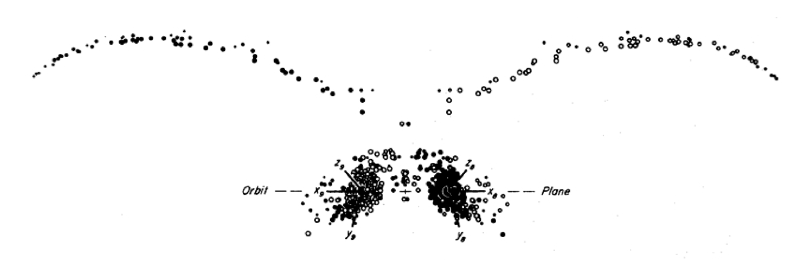
\includegraphics[width=0.8\textwidth]{Toomre.eps}
    \includegraphics[width=0.8\textwidth]{Antennae.eps}
    \caption[Early simulation of Antennae Galaxies]{The simulations of
    \citet{Toomre1972} showed how the kinematics of galaxy mergers can produce
    the variety of tidal structures seen in objects like the Antennae galaxies.
    The top image shows the result of one of the \citet{Toomre1972} simulations.
    \textit{Image credit: Adapted from figure 23 of \citet{Toomre1972}}
    The bottom image shows an observation of the actual object itself, the
    Antennae galaxies NGC 4038/4039. \textit{Image credit: NOAO/AURA/NSF, B.
    Twardy, B. Twardy, and A. Block (NOAO)}}
\end{figure}

The earliest numerical simulations of galaxy formation focused on the
effects of gravity alone.  A classic example of this are the simulations
presented in \citet{Toomre1972}, which showed that the irregular structures seen
in galaxies like NGC 4676 (``The Mice'') or NGC4038/4039 (``The Antennae
Galaxies'') are the results of major mergers between two disc galaxies.  These
simulations used discs composed of a mere 120 test particles, and ignored the
effects of self-gravity between these particles.  Despite the crudeness of these
simulations, these simulations definitively showed that galactic bridges and
tails could be formed by the tidal interactions of two passing/merging galaxies.
The IBM 360/95 that \citet{Toomre1972} (with an inflation-adjusted purchase
price in the millions of dollars) used for their simulations was capable of
5.5 million instructions per second, roughly $0.2\%$ the speed of the 35\$
Raspberry Pi 3 available today.

Modern galaxy simulations do far more than merely integrate the equations of
motion for a few hundred test particles in a gravitational field.  Today, state
of the art simulations will track gravity (including self-gravity) for stars,
gas, and dark matter; evolve Euler's equations for the hydrodynamics of gaseous
baryons; include models for radiative cooling of gas that allow for cooling from
both hydrogen and metal lines; form stars from dense gas; and include models for
feedback from massive stars and black holes.  Often, simulations will also
include treatments for radiative transfer and magneto-hydrodynamics as well.
Hydrodynamical solvers usually come in one of two classes: Eulerian or
Lagrangian.  Eulerian methods discretize space, breaking a simulation volume
into a grid of cells that each contains a number of scalar and vector quantities
that are advected according to the solver scheme.  Lagrangian methods instead
discretize mass, breaking the gaseous volume into discrete points, each of which
is moved to advect the quantities it contains, with smoothing functions used to
interpolate values in between particles.  Recently, new methods have begin to
hybridize features of each of these classes as well. Gravity is typically solved
using algorithms designed to minimize the workload that would be needed for a
direct summation of each particle or grid cell ($\mathcal{O}(N^2)$ for N grid
cells/particles).  Most codes use a tree-like or spectral algorithm to reduce
the cost to $\mathcal{O}(N\log{N})$, though a handful are beginning to adopt the
even faster Fast Multipole Method to reduce gravity calculation cost to
$\mathcal{O}(N)$.

In simulations of galaxies, the formation and deaths of individual stars are
typically unresolvable (in fact, this is currently true even for simulations of
molecular clouds).  This means that the formation of stars must be handled by
sub-grid approximations of the complex physics taking place at the sites of star
formation.  The simplest and most straight forward model is to simply assume
that gas will form stars at some fraction of the local free-fall time.  This leads
to a star formation rate that scales like $\dot \rho_* = c_* \rho_{gas}^{1/2}$,
where the single parameter $c_*$ is intended to capture the unresolved
efficiency of star formation at small scales.  

Modern galaxy simulations also now use a variety of strategies for judiciously
applying computational power where it is most needed.  Eulerian methods will
commonly use \textit{Adaptive Mesh Refinement} to increase resolution in regions of
interest (typically where gas is densest).  Lagrangian methods automatically do
this, as a denser region definitionally must contain more particles.  Beyond the
choice of algorithms, the choice of what type of simulation to set up in the
initial conditions is also important.  To study large populations of galaxies,
along with large-scale structure, large-volume cosmological boxes with
$>>10^4\;\rm{Mpc^3}$, but with spatial resolutions $\sim \rm{kpc}$ are used.
Studying how individual galaxies form is typically done with cosmological zoom
simulations, where a comparatively cheap dark-matter only simulation is first
run to select a region of interest, which is then resimulated with higher
resolution and baryonic physics included. Zoom-in simulations can typically
achieve an order of magnitude or better resolution than full cosmological boxes.
Isolated galaxy disc simulations cannot show how galaxies form in a cosmological
environment, but can be run with $\sim \rm{pc}$ resolution to study closely how
internal processes within a galaxy take place.

\section{The Importance of Feedback}
Simple analytic models for galaxy formation began with a universal picture of
their formation:  density perturbations that, over time, collapse under their
own self-gravity.  It is tempting to assume that this process dominates at all
scales of interest, as clearly stars form through the gravitational collapse of
gas clouds within the ISM (which themselves may form through their own
self-gravity).  This leads to a catastrophe at nearly all scales.  If gravity
is unopposed in star and galaxy formation, the timescales involved would scale
like the freefall time:
\begin{equation}
    t_{ff} = \sqrt{3\pi/32G\rho}
\end{equation}
The observed timescales for star and galaxy formation are much longer than this.
For galaxies, this predicts a complete conversion of gas to stars in $t_{ff} <<
t_{Hubble}$, which would mean the universe today would contain far more stars
than it does, and no actively star-forming galaxies.

We now know that galaxy and star formation is not a one
way process of gravitational collapse.  A number of internal processes
(``feedback'') within galaxies can liberate energy greater than the
gravitational binding energy of molecular clouds (and indeed even comparable to
the binding energy of the entire halo).  Early simulations that omitted
these feedback processes found that gas rapidly collapsed into the smallest
halos at high redshift, wildly overproducing stars in small galaxies at
high redshift (the ``cooling catastrophe'').  Galaxies like our own develop
unrealistically compact morphologies.  Simulations of individual molecular
clouds develop star formation rates an order of magnitude too high.  Aside from
establishing a number of observed galaxy properties, there are a observations of
feedback processes taking place.  Fast, massive outflows have been observed
leaving the discs of starburst galaxies and quasar host galaxies.  These
outflows must be powered by feedback.

\begin{figure}
    \includegraphics[width=0.8\textwidth]{M82.eps}
    \caption[Massive outflows in M82]{The evidence for feedback is no clearer
    than here in the Cigar Galaxy, M82.  The Hubble Space Telescope reveals
    massive outflows of hot ionized gas through the red $H\alpha$ emission seen
    as gas is blasted out of the galaxy in a bipolar flow. \textit{Image credit:
    NASA, ESA and the Hubble Heritage Team STScI/AURA}}
\end{figure}

Feedback energy may come from a number of sources.  The two primary sources are
massive stars and supermassive black holes (SMBHs).  Massive stars ($M>5M_\odot$)
live short, violent lives.  During their lives, they will drive fast
$v>1000\;\rm{km/s}$ stellar winds, and heat their surrounding gas with UV
radiation.  At the end of their lives $4-30\;\rm{Myr}$ later, these stars die in
extremely energetic core-collapse supernovae, liberating $\sim10^{51}\;\rm{erg}$.
This energy imparts heat and momentum to the surrounding ISM, and can accelerate
cosmic rays in the shocks that are driven.  In galaxies with actively growing
SMBHs, the accretion disc that forms as gas funnels into the black hole can
reach temperatures exceeding $10^9\;\rm{K}$ through viscous heating.  This
makes these accretion discs some of the most luminous objects in the universe,
and can heat the gas that surrounds the galaxy to choke off the accretion of new
material to form stars.

On the galactic scale, feedback regulates star formation in two primary ways.
Energy and momentum deposited into the ISM can heat and disrupt the cool clouds
of gas which form stars.  If that feedback is vigorous enough, this gas can
actually be ejected from the disc into the circum-galactic medium (CGM).  This
limits star formation by simply removing the fuel for the process.  Both of
these processes must be happening to explain observations of low star
formation efficiencies in molecular clouds, outflowing gas, a metal-polluted
intergalactic medium, and the low bulge fraction in star forming galaxies.

The greatest difficulty with including the effects of feedback in simulations of
galaxy evolution is the combination of extreme energy gradients in a relatively
small mass/volume.  Without overwhelmingly high resolution, hot feedback gas
will be numerically mixed with cold ISM, often resulting in gas with
temperatures of $\sim10^5\;\rm{K}$, at the peak of the ISM cooling curve where
cooling times are extremely short.  This results in feedback energy being
completely lost due to radiative cooling.  Indeed, as \citet{Thacker2000}
showed, how feedback energy is deposited into the ISM has a huge impact on
whether that feedback has any impact.  This problem has been tackled using a few
different strategies.  Since overcooling is the problem, many models have
attacked this directly by either temporarily disabling cooling
\citep{Stinson2006} or depositing feedback energy into a second, nonthermal
energy component \citep{Agertz2013}.  While this does limit radiative losses, it
produces gas that exists in an unphysical region of the $\rho-T$ phase diagram,
which may not have the correct entropy to escape buoyantly.  It also has the
potential to introduce an \textit{undercooling} problem as resolution becomes
higher and feedback-heated gas becomes resolvable.  Alternatively, energy may be
injected not as heat, but as momentum, which naturally does not cool.
Unfortunately, this adds the additional complexity of momentum cancellation (how
to treat neighbouring stars/clusters?), and if this momentum results in strong
shocks, these shocks will convert the momentum right back into thermal energy
that can radiate away the feedback energy the model is designed to preserve.
This often means kinetic/momentum feedback models must be combined with
hydrodynamic decoupling that renders feedback-heated gas into a form that does
not interact with the surrounding ISM.  Naturally, this makes outflow properties
strongly influenced by numerical choices.  

A third choice is to stochastically deposit feedback energy only when enough
energy is available to raise gas temperatures high enough for cooling times to
be short \citep{DallaVecchia2012,Crain2015}.  In these models, supernovae events
are effectively grouped together, somewhat decoupling feedback from star
formation.  The choice of temperature to heat gas to is a purely numerical
parameter, and can dramatically change the effectiveness of these models.
Finally, some \citep{Springel2010} attempt to directly address the unphysical
numerical mixing of hot and cold gas by separating the two phases and tracking
each component separately.  This completely solves the overcooling problem, and
allows the two components to cool radiatively.   Unfortunately, it also means
that cold star-forming gas is permanently coupled to hot feedback-heated gas:
effectively making the ISM an anchor holding down potential hot outflows.  This
means these multiphase models have to be coupled with parameterized models to
capture outflows.  Often, these simple models simply choose a fraction of
feedback energy to be deposited as kinetic ``kicks'' to a some gas particles.
Like other kinetic feedback models, this is frequently combined with
hydrodynamical decouplings.

All of these models attempt to solve the problem of overcooling with unphysical
approximations: disabled cooling, hydrodynamic decoupling, and stochastic
deposition of feedback energy.  These choices make it difficult to understand
what details of simulated galaxy evolution are a result of these numerical free
parameters, as opposed to the actual physics of feedback-regulated star
formation and outflows.  What is needed is a model that captures the effects of
feedback while matching as closely as possible the actual physical processes
involved below the resolution scale.

\section{Superbubble Feedback}
The formation of massive stars takes place mostly in clusters of $10^4$ or more
stars.  This means that the supernovae of these stars can be treated not as
individual dumps of $10^{51}\;\rm{erg/SN}$, but instead as a luminosity of
$10^{38}\;\rm{\frac{erg}{s \cdot M_\odot}}$.  This allows us to use stellar wind
models like \citet{Weaver1977} to study the evolution of superbubbles driven by
clustered supernovae.  Each individual supernovae's eject thermalizes in a small
region within the center of the bubble, and the resulting hot gas drives a shock
that sweeps up the surrounding ISM.  In a short time, the swept-up ISM can
efficiently radiatively cool, resulting in a thin, cold shell surrounding a hot
bubble.

The evolution of these superbubbles was studied in detail in \citet{MacLow1988}.
A key insight was that the hot bubble would evaporate the cold shell through
thermal conduction.  In a hot ionized plasma, electrons are able to penetrate
temperature gradients and deposit energy within cooler material, and via charge
conservation, establishing a mass flux against the temperature gradient.  This
evaporation means that the hot bubble with radius $R$ gains mass at a rate of:
\begin{equation}
    \frac{{\rm d }M_b}{{\rm d}t} = \frac{16\pi\mu}{25k_B} CT^{5/2}R
\end{equation}
Where $C=6\times10^{-7}\;\rm{erg\;s^{-1}\;cm^{-1}\;K^{7/2}}$, and $\mu$ is the
mean molecular weight of the gas in the bubble.  As the cold, evaporated
material acts to cool the hot bubble, this makes the bubble's interior
temperature self-regulating: higher temperature give higher mass flux, cooling
the bubble.

\citet{DallaVecchia2012} showed that the temperature of feedback-heated gas can
ultimately determine its effectiveness in driving outflows and regulating star
formation, even with constant feedback energy.  The self-regulating temperature
of superbubbles suggests that nature has a mechanism for setting
this temperature: thermal evaporation.
\bibliographystyle{mnras}
\bibliography{library}


\chapter{A Superbubble Feedback Model for Galaxy Simulations}
\thispagestyle{fancy}
\textit{Reprinted from B.W. Keller, J. Wadsley, S.M. Benincasa, \& H.M.P.
Couchman 2014,} \\ \textsc{Montly Notices of the Royal Astronomical Society}
\textit{Volume 442, Issue 4, pp. 3013-3025, DOI: 10.1093/mnras/stu1058.
Published by Oxford University Press on behalf of the Royal Astronomical
Society.  All rights reserved}
%\setcounter{pageFix}{\value{page}}
\begin{abstract}
\thispagestyle{fancy}
    \setcounter{page}{\value{pageFix}}
        \addcontentsline{toc}{section}{Abstract}
We present a new stellar feedback model that reproduces superbubbles.
Superbubbles from clustered young stars evolve quite differently to individual
supernovae and are substantially more efficient at generating gas motions.  The
essential new components of the model are thermal conduction, sub-grid
evaporation and a sub-grid multi-phase treatment for cases where the simulation
mass resolution is insufficient to model the early stages of the superbubble.
The multi-phase stage is short compared to superbubble lifetimes.  Thermal
conduction physically regulates the hot gas mass without requiring a free
parameter.  Accurately following the hot component naturally avoids overcooling.
Prior approaches tend to heat too much mass, leaving the hot ISM below $10^6$ K
and susceptible to rapid cooling unless ad-hoc fixes were used.  The hot
phase also allows feedback energy to correctly accumulate from multiple,
clustered sources, including stellar winds and supernovae.

We employ high-resolution simulations of a single star cluster to show the model
is insensitive to numerical resolution, unresolved ISM structure and suppression
of conduction by magnetic fields.  We also simulate a Milky Way analog and a
dwarf galaxy.  Both galaxies show regulated star formation and produce 
strong outflows.
\end{abstract}

\section{Introduction}
Galaxies are star factories:  with their large potential wells, they accrete gas
and convert that gas into stars.  The throttle for this process
is the energy released from these stars through winds and supernovae: stellar
feedback.  Without this large source of energy ($\sim 3\times 10^{38}$ erg
s$^{-1}$ per solar mass of stars) to stir and heat the interstellar medium, star
formation would consume all available gas for every galaxy in less than a Hubble
time.  Not only does stellar feedback allow star formation to self-regulate, it
is one of the most important processes in producing a multiphase ISM
\citep{McKee1977}.  A third way feedback shapes the history and structure of gas
in a galaxy is by cycling (and even ejecting) gas through outflows.  Galactic
winds can remove potential star-forming gas from a galaxy by propelling it out
of a galaxy faster than the escape velocity.  Gas `fountains' can reduce the
cold gas available in a galactic disc by cycling it between the disc and high in
the galactic halo. This acts to temporarily store gas in a reservoir above the
galactic plane, where it is too hot and diffuse to form stars.  These outflows
are likely an important component in determining the ultimate fate of a galaxy,
and are the most plausible mechanism for metal enrichment observed in the
circumgalactic medium \citep{Songaila1996,Dave1998}.

Much work has been done to build feedback models based on the evolution of
individual supernova blastwaves \citep[e.g.][]{Stinson2006}, but these efforts
have overlooked two key factors.  First, star formation is clustered; new stars
are spatially and temporally correlated, and feedback from their individual
winds and supernovae merge, thermalize and grow as a {\it superbubble} rather
than a series of isolated supernovae.  Second, because superbubbles have both
hot gas $>10^6\;\mathrm{K}$ and sharp temperature gradients, thermal conduction
is significant \citep{Weaver1977}.
Omitting this process can cause one to
incorrectly estimate the interior density (and thus the amount of hot gas) of
superbubbles by orders of magnitude, regardless of whether or not one can
resolve the superbubble.  In simulations of galaxy evolution, the temporal
resolution required to resolve the pre-thermalization Sedov phase is out of
reach (on the order of $100\;\mathrm{yr}$), and even the post-thermalization
early superbubble can require shorter timesteps than are practical. Worse still,
during this period the amount of mass contained within the hot, rarefied
interior of a superbubble is less than the mass of the progenitor star cluster.
This can make it impossible to spatially resolve this stage in simulations where
resolution elements are comparable in mass to star particles.  This leads to
denser, cooler feedback regions.  These overcool and lead to ineffective
feedback overall \citep{Katz1992}.

A number of approaches exist to attack the problem of overcooling.  The earliest
techniques were to simply deposit a fraction of the energy released in feedback
events as kinetic energy (\citet{Navarro1993}, \citet{Mihos1994},
\citet{Dubois2008}, etc.).  \citet{Gerritsen1997} detailed a second approach; by
introducing cooling shutoff, where feedback-heated gas is explicitly prevented
from cooling radiatively, and \citet{Thacker2000} explored a range of different
times for this shutoff period.  \citet{Stinson2006} proposed using the time
required to resolve a Sedov-Taylor blastwave, and showed that this can be an
effective way of modelling feedback in cosmological simulations of galaxy
evolution.  \citet{Agertz2013} used a decaying non-cooling energy, where energy
in a non-cooling state decayed back to the `normal' cooling form. Another
technique is to manually decouple density estimates and hydrodynamic
interactions between feedback-heated gas and the cold ISM (\citet{Marri2003},
\citet{Scannapieco2006}, etc.).  
With extremely high resolution, it
is possible to generate rarefied hot gas from feedback directly without 
a subgrid treatment \citep[e.g.][]{Hopkins2012b}.  
However, as we argue here, mass transfer between hot and cold gas
depends on the physics of conduction which relies on sub-parsec
gradients.  These are beyond the reach of even the highest resolution 
galaxy scale simulations so some subgrid modeling may be unavoidable.

Another approach has been to explicitly model the multiphase ISM
below the resolution limit.  \citet{Springel2003} described a multiphase
model based on the theoretical framework of \citet{McKee1977}.  Each
particle was composed of an isobaric mix of cold clouds and ambient warm
to hot gas.  Radiative cooling converts warmer gas into cold.  The cold
phase forms stars on a characteristic timescale chosen to yield a
Schmidt-type star formation law.  An empirical model of stellar feedback
evaporates the cold phase.  \citet{Springel2003} recognized that while
this model works well for simulating star formation and feedback in
quiescent galaxies, the coupling of hot and cold mass can prevent hot
gas from leaving the disc as winds or outflows.  Their solution was to
convert a fraction of the feedback energy in a kinetic kick on selected
particles, in the same vein as \citet{Mihos1994}.  

Both \citet{DallaVecchia2012} and \cite{Hopkins2012b} have shown
that it is possible to get consistent wind results for a given energy input model.   
\citet{DallaVecchia2012} demonstrated that simply depositing 
 energy stochastically to ensure a constant temperature increase for 
feedback-heated gas can directly generate winds.    
They found that for the same feedback energy,
changing the temperature of feedback-heated gas results in significant
differences in both star formation regulation and galactic outflows.  Higher
feedback temperatures, $\Delta T > 10^7\;\mathrm{K}$, avoid overcooling and
allow for more efficient regulation and higher velocity galactic winds.  
This still leaves open the question of what sets this temperature?  
This question is equivalent to asking: {\it what sets the mass-loading in stellar
feedback?}   Previous feedback models have not explored key
physical mechanisms, such as conduction, that affect mass-loading.

The above sub-grid models are reasonably successful at preventing
overcooling.  However, many of them have limitations which are
increasingly severe with improving resolution.  For example, stellar feedback
in the form of kinetic energy is rapidly converted into thermal energy as it
encounters the ISM and shocks \citep{Durier2012}.  In nature,
the gas heated by feedback doesn't completely stop cooling radiatively, it
merely cools inefficiently.  Applying a cooling shutoff is unlikely to give the
correct behaviour in different star forming environments and is also dependent
on the integrated energy injection from all nearby stars.  Finally, because
star formation is clustered, feedback is localized within starforming regions. 

Recent studies such as \citet{Nath2013} and \citet{Sharma2014} have emphasized
that feedback from clustered stars forms superbubbles, which behave quite
differently from isolated supernovae.   A key outcome is that superbubbles are
intrinsically more efficient than individual supernovae at converting feedback
energy into gas motions, particularly at late times and over larger scales.  The
reason for this difference is that gas heated by feedback remains distinct from
the cooler surrounding material.  Most current models smear together the hot
bubble with the cold shell surrounding it.  This results in an intermediate
effective temperature that is prone to overcooling.   Separating the hot and
cold phases automatically avoids overcooling.  \citet{DallaVecchia2012} achieved
this with a stochastic feedback model.  An alternative approach is to add an
explicit hot reservoir to accumulate feedback mass and energy.  This avoids
overcooling without artificially turning off cooling and correctly handles
feedback from multiple sources over time without resorting to a stochastic
approach.  Such a model still leaves the bubble mass as a free parameter.
\citet{MacLow1988} showed that thermal conduction controls the mass flow into
the hot bubble from the cold shell.  This evaporation process regulates the
temperature of the hot bubble and determines how much mass is heated by
feedback.   Adding a sub-grid model for evaporation allows the physics of
thermal conduction to set bubble temperatures and masses.

Drawing on these facts, we can construct a {\it superbubble}-based feedback
model.  As outlined in \citet{MacLow1988}, superbubbles efficiently convert
feedback energy into thermal energy in a hot phase and kinetic energy in an
expanding cold shell.  The rarefied hot phase cools inefficiently, avoiding
overcooling.  Thus a correct model requires following distinct hot and cold
phases even when they may be difficult to resolve directly.  A new requirement
with respect to prior feedback models is the inclusion of thermal conduction.
Conduction both smooths the temperature distribution in the hot gas and mediates
mass flows where hot gas meets a cold phase.  Thus a second feature of such a
model is that an explicit physical process sets the amount of hot gas in the ISM
and in outflows.

In this paper, we begin by explaining the theoretical underpinning and
numerical implementation of the superbubble-based feedback method in
section~\ref{method1}. 
In section~\ref{cluster1} we use a single star cluster to illustrate the
effectiveness of our model at capturing the basic behaviour of superbubbles at
high and low resolution.  In section~\ref{galaxy1} we apply the model to
simulations of isolated galaxies to explore the impact on the galaxy
scale ISM and the production of outflows.  

\begin{figure*}
    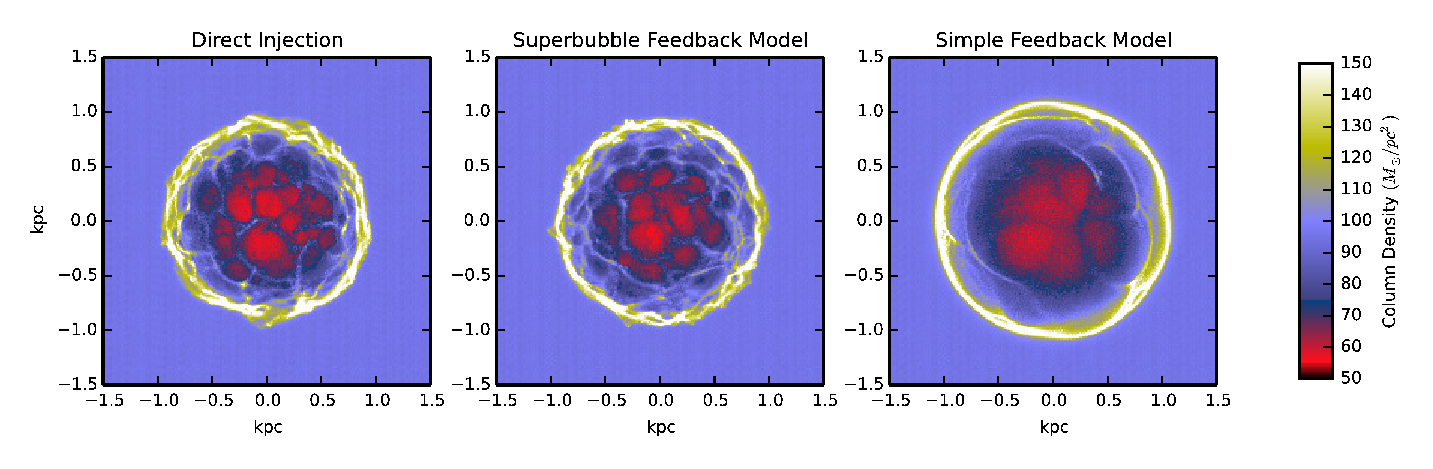
\includegraphics[width=\textwidth]{figures1/onestar_column.eps}
    \caption[Column density plot of a superbubble from a single cluster]{Column
    density projections from the simulations of a single star cluster with mass
    $3\times10^4\;\mathrm{M_\odot}$, $50\;\mathrm{Myr}$ after the cluster has
    formed.  The superbubble feedback model (center column) produces bubbles
    with radius and enclosed mass that match well to the direct injection
    simulations (left column).  This is shown quantitatively in
    figure~\ref{onestar_homogeneous1} and figure~\ref{onestar_clumpy1}.  The
    simple model (right column), despite injecting the same amount of energy,
    fails to generate enough hot mass inside the bubble, and subsequently
    suppresses the growth of Vishniac instabilities along the bubble edge
    because of the poorly resolved hot interior.}
    \label{onestar_column1}
\end{figure*}


\section{Thermal Conduction and Feedback Method}\label{method1}
Our new treatment of feedback has three components.  The first is the addition
of thermal conduction.   Inside resolved hot bubbles, thermal conduction
maintains uniform temperatures.   In the presence of strong gradients, thermal
conduction can lead to evaporative mass flows from cold to hot gas.  The second
component is a stochastic model of evaporation to allow resolved hot gas to
continue to gain mass from nearby cold gas.  Thus, the amount of cold gas heated
by feedback is not a free parameter, but is set by thermal conduction.  
Without a mechanism like thermal conduction, this hot gas mass is set by
how many fluid elements have feedback energy deposited into them.   It is
important to note that in our model these processes operate everywhere
temperatures are above $10^5K$. 

Finally, in the first few $\mathrm{Myr}$ of feedback heating, the mass contained
within a hot bubble can be smaller than the simulation gas mass resolution.  To
prevent overcooling, we allow resolution elements to become briefly two-phase; a
hot interior (bubble) in contact with a cold shell.  Evaporation of the cold
shell moderates this two-phase period, rapidly returning particles to single
phase once their cold phase has been fully evaporated.  Our model does not
assume all fluid elements are multiphase, but only those in which a partial
feedback region exists.  This allows the model to follow winds and outflows
without continuing to rely on sub-grid machinery.  

Young stellar populations steadily release energy in the form of winds and SNe at
a rate of $3\times 10^{38}\;\mathrm{erg\; s^{-1} M_\odot^{-1}}$ for around 40
Myr~\citep{Leitherer1999}. We deposit this energy into the gas particle nearest
to the star particle.  In following with past work, we use the feedback rates
and times for supernovae, but the method is general enough to handle heating
from stellar winds, ionization, etc.  Heating takes effect
$4\;\mathrm{Myr}$ after a star forms, and continues until $30\;\mathrm{Myr}$
after the star particle forms (the time associated with SNII from OB stars).  Thus,
each supernova releases $10^{51}\;\mathrm{erg}$, and each star particle will
release $10^{49}\;\mathrm{erg M^{-1}_\odot}$ using the \citet{Chabrier2003} IMF.

\subsection{Thermal Conduction}
In an ionized gas, thermal conduction, mediated by electrons,
transports heat down temperature gradients.  This flux, $\mathbf{Q} =
-\kappa\nabla T$, depends on the temperature gradient and the conduction
coefficient, as derived by \citet{Cowie1977},
\begin{equation} \label{coefficient1}
    \kappa(T) = 1.8\left(\frac{2}{\pi}\right)^{3/2}\frac{T^{5/2}k_B^{7/2}}{m_e\,e^4\ln\Lambda}.
\end{equation}
This coefficient depends only on the Coulomb logarithm $\ln\Lambda$ (which has
an extremely weak dependence on density), and is well approximated by $\kappa(T)
= \kappa_0\,T^{5/2}$, where $\kappa_0$ is $6.1\times10^{-7}\;\mathrm{erg\;s^{-1}
K^{-7/2}cm^{-1}}$ in the absence of magnetic fields.  This drives a
corresponding mass flux, {\it in the opposite direction}.  With spherical
symmetry, this implies a mass flow rate that depends on the sound speed in the
hot gas, $c_{\rm s}$, as follows,
\begin{equation}\label{conservation1}
    \frac{5}{2}\dot M c_{\rm s}^2 = 4\,\pi^2r^2\kappa(T)\frac{{\rm d}T}{{\rm d}r}.
\end{equation}

These rates hold only when the mean free path of electrons in the medium is
smaller than the scale length of the temperature gradient.  If the gradient
becomes steep enough, the heat flux (and corresponding mass flux) saturates at a
value that depends only on the density, temperature, and thermal velocity of the
electrons in the medium \citep{Cowie1977},
\begin{equation}\label{heatflux1}
    \mathbf{Q} = \nabla\left(\frac{3}{2}n_ek_BT_ev_e\right).
\end{equation}
This saturation has the convenient numerical side effect of setting the smallest
timestep required to resolve this mass flux to $\sim 1/17$ the standard Courant
time, $t_C = \Delta x /c_s$.

In situations where the temperature gradient is embedded in a strong magnetic
field, the value of $\kappa_0$  can be reduced by factors approaching an order
of magnitude depending on the strength and configuration of the magnetic fields
\citep{Cowie1977}.

The edge of a feedback-driven superbubble presents a strong discontinuity in
both temperature and density.  Interior to the bubble, gas has temperatures of
$\sim 10^6\;\mathrm{K}$ and densities of $\sim10^{-3}\;\mathrm{cm^{-3}}$, while
the shell can have temperatures below $100\;\mathrm{K}$ and densities of $\sim
10\;\mathrm{cm^{-3}}$ \citep{Chevalier1974}.  This generates significant mass
and energy flows due to thermal conduction.

\subsection{Evaporation}
The dominant physical process governing mass flux between the hot and cold
phases of a feedback bubble is thermal conduction between the dense shell and
the hot interior.   As this process takes place on length scales far below the
resolution limit, we must capture its effects in a subgrid model.  For the thin
shell surrounding a feedback bubble, thermal conduction causes an evaporative
mass flux from the cold shell into the hot bubble.  Following
\citet{MacLow1988}, the mass flux into a bubble with interior temperature $T$
is,
\begin{equation}\label{massflux1}
    \frac{{\rm d }M_b}{{\rm d}t} = \frac{4\,\pi\mu}{25k_B}\kappa_0\,\frac{\Delta T^{5/2}}{\Delta x}\ A,
\end{equation}
where $A$ is the bubble surface area and $\Delta x$ is the thickness of the hot
layer ($\Delta x = R$ for spherical symmetry).  For the Smoothed Particle
Hydrodynamics (SPH) method used for our tests, we calculate evaporation using
the outer layer of hot particles bordering the cold gas.  The members of this
layer are those with no other hot particles within $45^o$ of the vector to the
centre of mass of their cold neighbours.  As we cannot directly determine the
radius of a well-resolved superbubble without expensive non-local calculations,
we need a way to allow each particle to estimate the radius and thus its
fractional contribution of the shell surface area.  The total area estimated by
all hot particles in a bubble should approach $\sim 4\pi R^2$ where $R$ is the
bubble radius.  For a poorly resolved bubble $R \sim 1-2\,h$, where $h$ is a hot
particle's SPH smoothing length.  For larger bubbles each hot particle
contributes an area of $\sim h^2$ and each particle sees a nearly plane-parallel
section of the cold shell.  We examined a number of bubbles at different stages
of growth, as well as a plane-parallel slab, and empirically found that a good
per-particle area estimate was $A = \frac{6\,\pi\,h^2}{N_{\rm hot}}$, where
$N_{\rm hot}$ is the number of hot neighbours for that particle and $\Delta x =
h$.  We stress that this is a fit for our specific SPH neighbour approach
(described below) that should be recalibrated for other codes.

The mass evaporation rate can be converted into a probability that a resolution
element with cold mass $m$ converts into a hot one over a time
period $\Delta t$ as follows, 
\begin{equation}\label{evaporation_probability1}
    P_{evap} = \frac{{\rm d}M_b}{{\rm d}t} \frac{\Delta t}{m}.
\end{equation}
This allows us to stochastically choose full particles to evaporate, and prevent
overcooling due to fractional particle evaporation (exactly the same overcooling
problem seen in feedback heating).  Each hot particle determines how many
cold-shell particles $N_{evap}$ will evaporate each timestep, and then chooses
the $N_{evap}$ nearest cold particles, and averages the thermal energy of itself
and those particles.  These particles spontaneously join the hot bubble
(demonstrated in the figures in section~\ref{clumpy1}).  The thermal conduction
rates calculated are capped using the saturation values derived in
\citet{Cowie1977}.  Within an SPH framework, this is well approximated using,
\begin{equation}\label{saturation_rate1}
    \frac{{\rm d}M_{sat}}{{\rm d}t} = 17\rho\,c_{\rm s} h^2.
\end{equation}

\begin{figure*}
    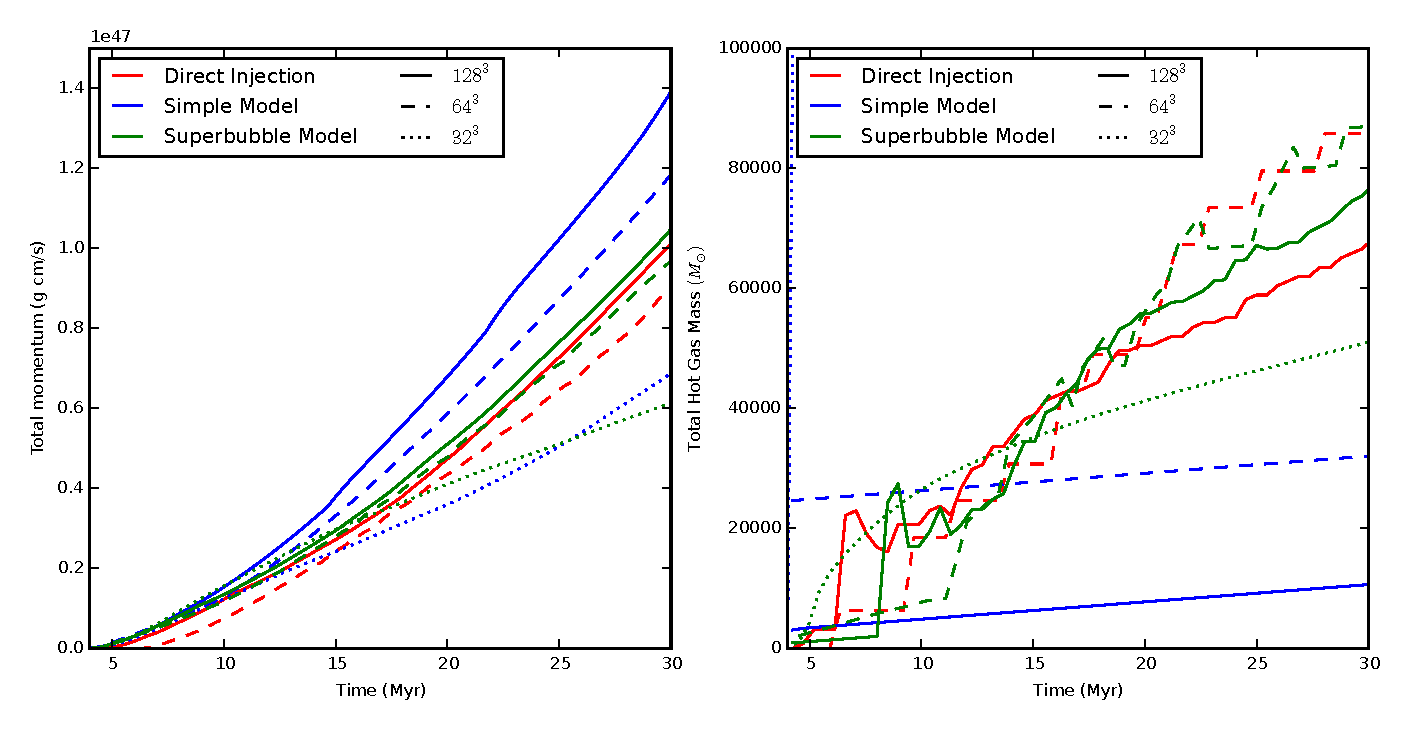
\includegraphics[width=0.8\textwidth]{figures1/onestar_homogeneous.eps}
    \caption[Feedback effects as a function of resolution]{Feedback effects as a
    function of resolution.  The above figure shows on the left the total radial
    momentum imparted to the medium, and on the right the total amount of mass
    heated to above $10^5\;\mathrm{K}$.  The red curves are the direct injection
    results, the blue corresponds to the simple feedback, while the green shows
    the results of the superbubble model.  Solid lines show the values from
    simulations run with resolutions of $128^3$ particles, dashed for $64^3$,
    and dotted for $32^3$.  Note that for the $32^3$ run, the simple model
    produces $\sim 2\times 10^5\;M_\odot$ of hot gas.}
    \label{onestar_homogeneous1}
\end{figure*}

\subsection{Multiphase Fluid Elements}
When feedback energy is deposited in a low-resolution simulation, or is
deposited as a luminosity, the temperature and density are certain to be under-
and over-estimated respectively.  This problem leads to the well-known
overcooling problem that has typically been addressed by disabling
cooling for some amount of time for feedback-heated gas (e.g.
\citet{Stinson2006}, \citet{Springel2003}, or by stochastic feedback heating,
where the temperature change of a fluid element heated by feedback is fixed to a
constant value (e.g.  \citet{DallaVecchia2012}.  We employ a third option:
storing feedback energy in a second phase that is in pressure equilibrium with
the rest of the fluid inside an element.

Fluid elements (gas cells or particles) enter the multi-phase state if they are
given energy from feedback, and if their temperature is below $10^5\;\mathrm{K}$
(the `hot' threshold).  Multiphase elements have two values for their mass and
energy, related to their total mass $m$ and energy $E$ by:

\begin{equation}\label{multiphase_fractions1}
    m = m_{\rm hot}+m_{\rm cold}
\end{equation}
\begin{equation}
    E = u_{\rm hot}m_{\rm hot}+u_{\rm cold}m_{\rm cold}
\end{equation}

Assuming pressure equilibrium, both phases will have the same pressure $P$, and
their densities are found using this and the total density $\rho$:
\begin{equation}\label{multiphase_pressurebalance1}
    \frac{P}{\rho} = \frac{(\gamma-1)E}{m}
\end{equation}
\begin{equation}\label{multiphase_densities1}
    \rho_{\rm cold} = \frac{P}{(\gamma-1)u_{\rm cold}}
\end{equation}
\begin{equation}
    \rho_{\rm hot} = \frac{P}{(\gamma-1)u_{\rm hot}}
\end{equation}

Both the cold and hot phases are allowed to radiatively cool using their
separate temperatures and densities.   When $PdV$ work is done to a multiphase
particle, it is shared between the two phases weighted by their respective
fraction of the total energy E,
\begin{equation}\label{multiphase_PdV1}
    \dot u_{\rm PdV,cold} = m\ \dot u_{\rm PdV}\frac{u_{\rm cold}}{E}\\
\end{equation}
\begin{equation}
    \dot u_{\rm PdV,hot} = m\ \dot u_{\rm PdV}\frac{u_{\rm hot}}{E}.
\end{equation}
In the absence of heating and cooling, this allows each phase to correctly
maintain constant entropy as the densities change.

Mass flux between the hot and cold phase is calculated in a continuous manner
consistent with the prior evaporation scheme.  Each timestep, a multi-phase
element evaporates a fraction of its cold phase into the hot phase,

\begin{equation}\label{multiphase_evaporation1}
    \frac{{\rm d}M_b}{{\rm d}t} = \frac{16\pi\mu}{25k_B} \kappa_0 (T_{\rm hot}^{5/2})\ h.
\end{equation}

Once an element has evaporated all of its mass into the hot phase, or if the hot
phase cools below $10^5\;\mathrm{K}$, it is returned to the single-phase state.

\subsection{SPH Implementation}

We implemented this method in the SPH code {\sc GASOLINE}
\citep{Wadsley2004} with updates described in \cite{Shen2010}.  These
include a sub-grid model for turbulent mixing of metals and energy.  The
heating and cooling include photoelectric heating of dust grains, UV heating
and ionization and cooling due to hydrogen, helium and metals.

The SPH hydrodynamic treatment has had some further, key updates.  We currently
use a standard SPH density estimator but a  geometric density average in the SPH
force expression: $(P_i+P_j)/(\rho_i\,\rho_j)$ in place of
$P_i/\rho_i^2+P_j/\rho_j^2$ where $P_i$ and $\rho_i$ are particle pressures and
densities respectively. This force expression alleviates numerical surface
tension associated with density discontinuities, which is important for correct
Kelvin-Hemholtz instabilities and ablation of cold blobs (as in the Agertz et al
2010 'blob' test).  A similar force expression was first proposed by
\citet{Ritchie2001}.  Geometric density averaged force expressions are now
employed in all modern SPH codes (e.g. \cite{Hopkins2013}, \cite{Saitoh2013},
\cite{Kawata2013}, \cite{Hu2014} and \cite{Read2010}).  As
stated in \cite{Read2010} and \cite{Saitoh2013}, a key requirement
for correct results with the modified force expression is a consistent energy
equation that conserves entropy (which we employ).  This is important to
correctly model strong shocks, such as Sedov blasts.  The extreme temperature
jumps at strong shocks also require the time-step limiter of \citet{Saitoh2009}.
The modern SPH code papers listed above all employ these updates and demonstrate
accurate solutions for strong shocks (e.g. Sedov blasts) and shear flows (e.g.
Kelvin Helmholz instabilities and the destruction of cold blobs).

For the tests shown here we used the Wendland $C_2$ kernel detailed in
\citet{Dehnen2012} with 64 neigbours where the SPH smoothing distance is defined
so that the kernel weight drops to zero at $2\,h$.  

Sharp density contrasts, as seen in highly resolved superbubbles, can require
additional checks on the neighbour finding component of the SPH method.  For
example, hot particles can inadvertently become hydrodynamically decoupled from
cold ones for a fixed number of neighbours.  A full set of cold neighbours can
sit at the edge of the kernel, where their contribution is negligible.  The hot
particle can thus have a full set of neighbours but feel minimal forces.  We
increase the number of neighbours until at least $18$ neighbours are within
$1.41\,h$.  

With respect to heating and cooling, for this work we used the
\citet{Ritchie2001} density when calculating cooling rates to sharpen the
density contrast between hot and cold gas.  This is particularly useful at lower
resolution when the hot bubble is resolved with a small number of particles.
This improves the ability of low resolution runs to give similar energy loss
rates to high resolution versions.
 
Feedback can increase gas particle masses substantially in the rare event that a
gas particle spends a lot of time within star clusters without forming a star
itself.  This can degrade the accuracy of the SPH method.  We avoid this problem
by splitting particles that exceed $4/3$ their initial mass into two equal mass
particles with the same properties.  This affects a very small fraction of the
particles.

These modifications, along with detailed testing, will be discussed in a
forthcoming paper on {\sc GASOLINE2}.  For reference, the quality of our results
on the tests discussed here is similar to the results presented for other modern
modified SPH codes \citep[e.g.][]{Hopkins2013}. 

\begin{figure}
    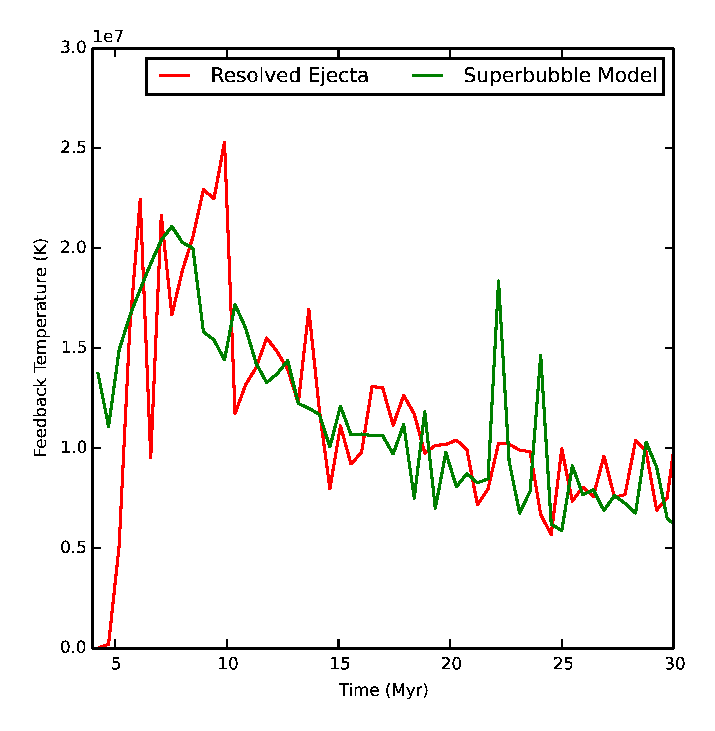
\includegraphics[width=0.5\textwidth]{figures1/onestar_hottemp.eps}
    \caption[Peak temperature of feedback-heated gas in a superbubble]{Peak
    temperature of feedback-heated gas inside the isolated star cluster's hot
    bubble.  Evaporation quickly enters the self-regulating regime, and the
    temperature is roughly constant for the last $15\;\mathrm{Myr}$ of
    feedback.}
    \label{onestar_hottemp1}
\end{figure}


\section{Simulations}
\subsection{High-Resolution Star Cluster Test}\label{cluster1}
We began by exploring models of a single, isolated superbubbles at high
resolution.  For these tests, we employed three physical models.  The {\it
Direct injection} approach models as much physics as possible from first
principles.  Feedback mass and energy is modelled via a stream of new gas
particles created from the star cluster.  This approach only works when the gas
resolution elements are much smaller than the star cluster mass.  The only
component of this model that is sub-grid is evaporation as this occurs on
extremely small length scales.  {\it Superbubble Feedback} refers to our new
model.  The key addition over the direct approach is the sub-grid multiphase
treatment.  Feedback energy and mass is injected into existing particles which
may split.  

We also include a {\it Simple Feedback
Model} modeled after that proposed by \citet{Agertz2013}.  This model is a
stand-in for models typically used to date and does not include conduction or
evaporation.  Feedback mass and energy is given to the nearest gas particle to
the star cluster.  This simple model incorporates a two-component energy
treatment with radiative cooling disabled for feedback energy.  Feedback energy
is steadily converted into the regular, cooling form with an e-folding time of
$5\;\mathrm{Myr}$. 

\subsubsection{Basic Superbubble}

We placed a star cluster with mass $3\times10^4\;\mathrm{M_\odot}$ in a uniform
periodic box $2\times2\times2\;\mathrm{kpc}$ in size, containing
$10^3\;\mathrm{K}$ gas with solar metallicity at a density of
$1\;\mathrm{cm^{-3}}$.   This gives a gas particle mass of $760\; M_\odot$,
$6080\; M_\odot$, and $48640\; M_\odot$ for resolutions of $128^3$, $64^3$, and
$32^3$ respectively.  These tests do not include photoheating. 

Figure~\ref{onestar_column1} shows the column density projection for the three
different feedback models in an isotropic medium.  The hot interior of the
bubble produced using the simple feedback model contains less mass at $128^3$
than the direct injection model and is subsequently too poorly resolved for the
instabilities formed in the accelerated shell \citep{Vishniac1983} to mix the
bubble and shell through turbulence and diffusion.

As figure~\ref{onestar_homogeneous1} shows, the superbubble feedback model
performs much better than the simple model in reproducing the hot mass
production rate from the high-resolution direct injection model, and lacks the
extreme resolution sensitivity that the simple model exhibits for the amount of
gas heated. The simple model only heats $\sim 4$ gas particles.  For the $128^3$
and $64^3$ resolutions, this gives too little hot mass.  For $32^3$ (extremely
poor resolution, in fact with gas particles more massive than the entire
cluster), this produces more than twice too much hot mass (more than
$2\times10^5\;M_\odot$). Meanwhile the simulation with the superbubble feedback
model only underestimates the hot mass by roughly a third of the target $128^3$
direct injection simulation when used at a resolution $32^3$.  The decreased
momentum in the lower-resolution runs is likely due to particles staying longer
in the multiphase state.  More massive particles take longer to fully evaporate,
and thus some mass that would be part of a pressure-driven cold shell at higher
resolution is tied up in the cold part of multiphase particles.

Figure~\ref{onestar_hottemp1}  shows that the actual peak temperature of the
feedback-heated bubble in the isolated star cluster run is roughly
$1\times10^7\mathrm{K}$.


\begin{figure}
    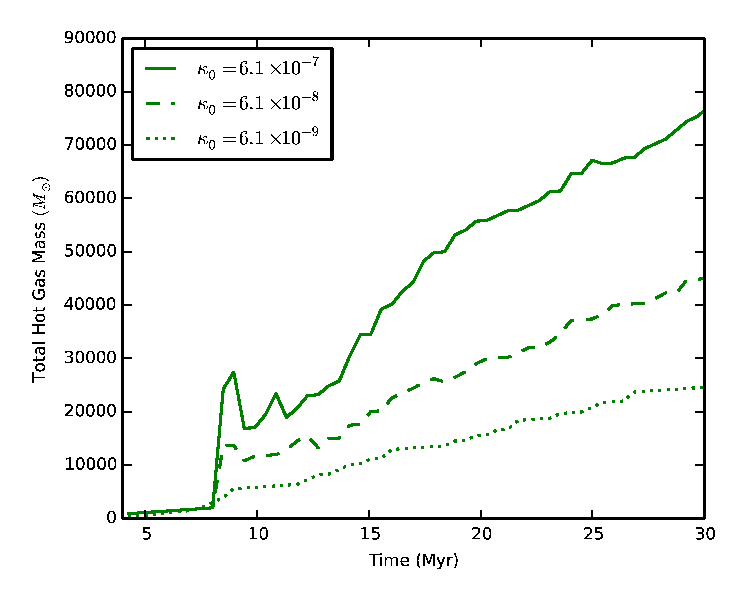
\includegraphics[width=0.6\textwidth]{figures1/onestar_kappa.eps}
    \caption[Dependence of superbubble heated gas on conduction coefficient]{Hot
    mass production as a function of the conduction coefficient $\kappa_0$.  As
    this figure shows, reducing $\kappa_0$ by a factor of 100 reduces the amount
    of hot mass generated through conduction by only a factor of $\sim2$. All
    $\kappa_0$ values have units of $\mathrm{erg\; s^{-1} K^{-7/2} cm^{-1}}$.}
    \label{onestar_kappa1}
\end{figure}

\subsubsection{Suppressed conduction}

We also ran a set of simulations with the value of $\kappa_0$ used in the model
reduced by a factor of 10 and a factor of 100.  Since there is some uncertainty
as to this coefficient in a magnetized ISM, we use this test to show that the
self-regulating effect of conduction is insensitive to variation in $\kappa_0$.

Figure~\ref{onestar_kappa1} shows the hot mass generated in simulations with 3
different values of $\kappa_0$.  The dashed curve shows a reasonable lower limit
for $\kappa_0$ \citep{Cowie1977}, while the dotted curve shows a much more
extreme conduction reduction than is expected in nature.  Both curves illustrate
the insensitivity of the method to reductions in the conduction rate.  Even
reducing $\kappa_0$ by 100 only results in a reduction of the hot mass inside
the bubble to just around a third.  


\begin{figure}
    \includegraphics[width=\textwidth]{figures1/onestar_clumpypoints.eps}
    \caption[Image of superbubbles in a clumpy ISM]{3 kpc wide slices
    from the same three methods shown in figure~\ref{onestar_column1}, also at 50
    Myr, but applied to a star cluster in an inhomogeneous medium.  Particles
    whose smoothing length intersects z=0~kpc are shown.  Particles above $10^5$
    K are shown in red.  The upper row shows simulations with a single clump,
    while the bottom row shows simulations with 6 clumps.}
    \label{onestar_clumpyslice1}
\end{figure}

\begin{figure*}
    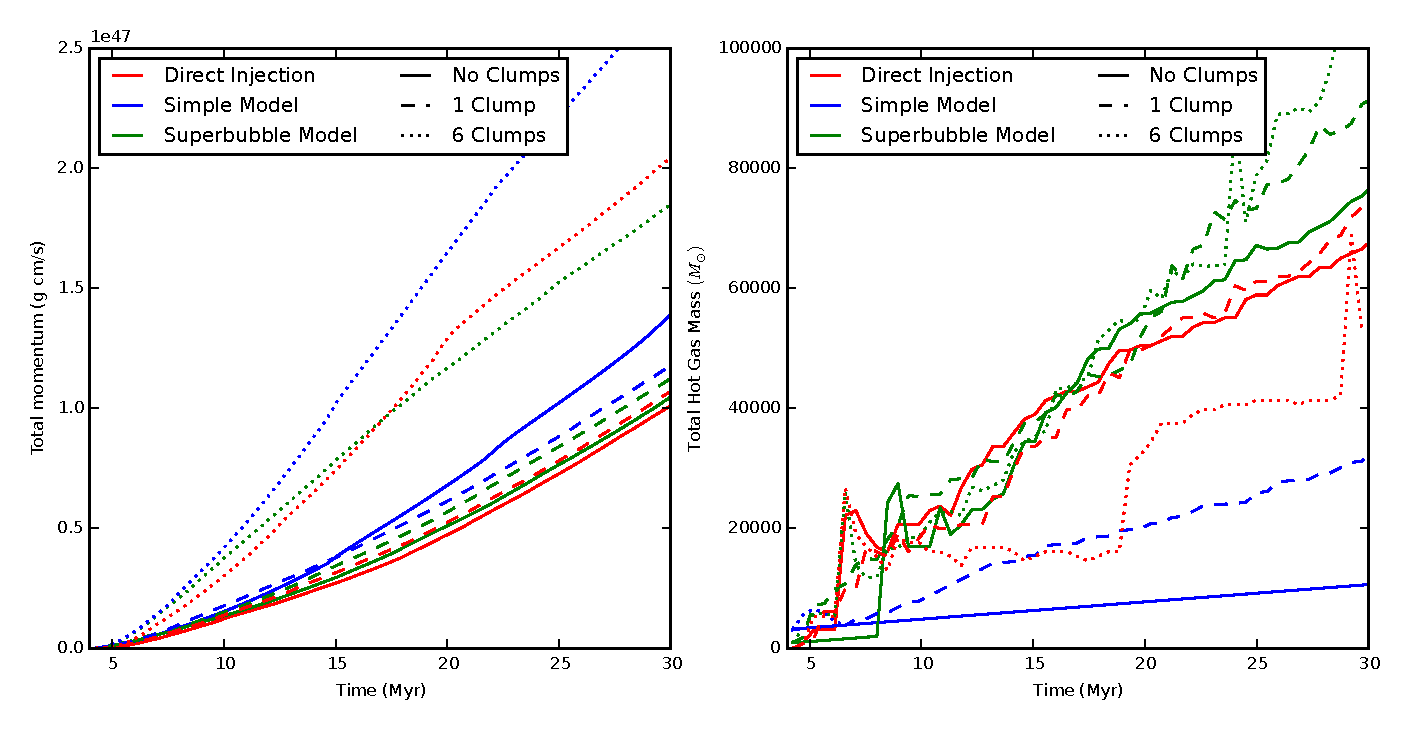
\includegraphics[width=0.8\textwidth]{figures1/onestar_clumpy.eps}
    \caption[Feedback effects as a function of ISM homogeneity]{Feedback effects
    as a function of ISM homogeneity.  The above figure shows on the left the
    total radial momentum imparted to the medium, and on the right the total
    amount of mass heated to above $10^5\;\mathrm{K}$.  The red curves are the
    direct injection results, the blue corresponds to the simple feedback, while
    the green shows the results of the superbubble model.  Solid curves show the
    results for a homogeneous ISM, dashed for a single dense clump, and dotted
    for 6 dense clumps.}
    \label{onestar_clumpy1}
\end{figure*}

\subsubsection{Clumpy Medium}\label{clumpy1}
As the real ISM is highly inhomogeneous (and as \citet{Silich1996} showed, cold
clumps can also be a source of evaporated cold material), we ran two additional
simulations with cold, dense clumps with $100\;\mathrm{cm^{-3}}$ density and
$10\;\mathrm{K}$ gas in an ambient medium of $0.5\;\mathrm{cm^{-3}}$ at
$1000\:\mathrm{K}$.  This gives roughly the same amount of mass enclosed within
the hot bubble at $30\:\mathrm{Myr}$.  The first contains a single spherical
clump with a radius of $0.2\;\mathrm{kpc}$.  The second contains the same amount
of cold mass spread over 6 clumps arranged at the center of each face of a cube
$0.2\;\mathrm{kpc}$ surrounding the star.  We use this idealized clumpy medium
to test the sensitivity of the model to small scale structure that may be
unresolved in lower resolution simulations. Figure~\ref{onestar_clumpyslice1}
shows a slice showing SPH particles at $50\;\mathrm{Myr}$ for the two clumpy
cases.  

Figure~\ref{onestar_clumpy1} shows that the superbubble model is also capable of
handling feedback into a clumpy medium.  With more than an order of magnitude
difference in the total hot mass compared to the simple model, along with less
sensitivity to environment or resolution, the superbubble model is better
suited for probing galactic outflows in simulations.  


\begin{figure*}
    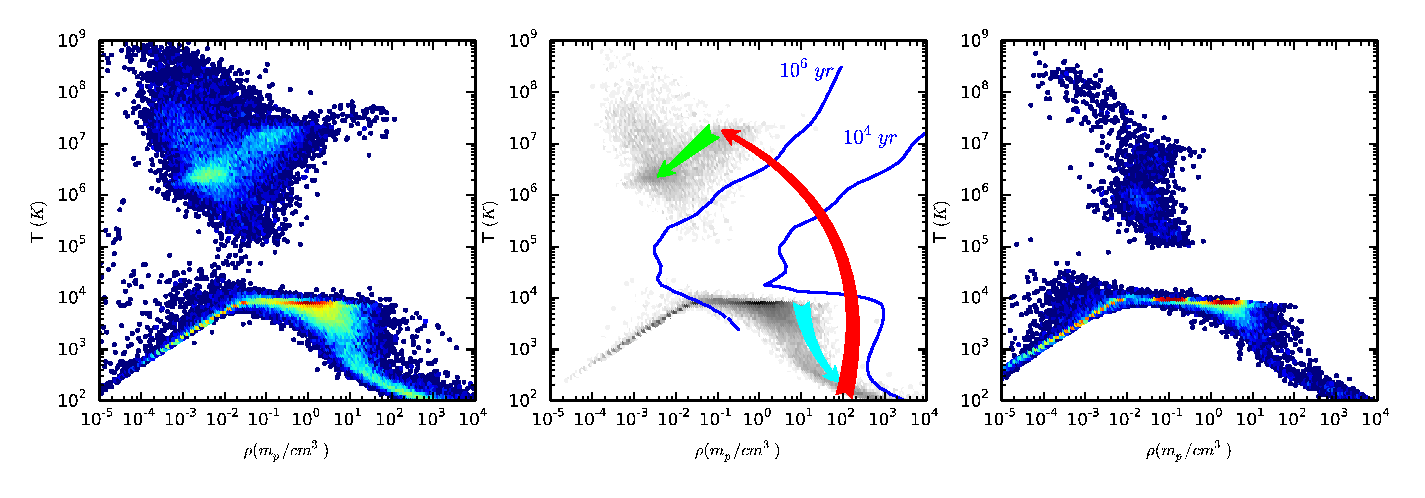
\includegraphics[width=\textwidth]{figures1/disc_phase.eps}
    \caption[Phase diagram of gas in isolated galaxies]{Phase diagrams for the
    Milky Way (left) and dwarf (right) simulations at $200\;\mathrm{Myr}$.  The
    central panel shows a typical path for gas ejected from the Milky Way.
    First gas cools radiatively (cyan path) to high density, where it becomes
    multiphase as its hot component is heated to $\sim10^7\;\mathrm{K}$ by
    feedback (red path) from nearby stars formed from its neighbouring high
    density gas.  The hot phase cools primarily through adiabatic expansion
    (green path).  This process is often repeated one or more times, with gas
    that is entirely hot phase being ejected from the disc.  Cooling times of
    $10^4\;\mathrm{yr}$ and $10^6\;\mathrm{yr}$ are shown in blue. The
    majority of the hot gas in the upper left quadrant of the phase diagram has
    cooling times $>10^8\;\mathrm{yr}$.  The cooling curve for
    $10^8\;\mathrm{yr}$ passes through the green curve.  Note that particles in
    the multiphase state show the temperature and density for each state as
    separate points.  The mean properties of multiphase particles would place
    them in regions with short cooling times.}
    \label{disc_phase1}
\end{figure*}



\subsection{Galaxy Simulations}\label{galaxy1}
\subsubsection{Initial Conditions and Parameters}
\begin{figure*}
    \includegraphics[width=\textwidth]{figures1/milkyway_column.eps}
    \caption[Column density and temperature images of isolated Milky Way]{Column
    Density (upper row) and temperature for the Milky Way simulation at
    $300\;\mathrm{Myr}$.  The vectors show the in-plane velocity.  Temperatures
    shown are averages between the two phases for multiphase particles.  Black
    points in the face-on images show stars formed within the last
    $20\;\mathrm{Myr}$. Note that gas is both leaving the disc near the galactic
    core, and returning in some places near the edge.}
    \label{milkyway_column1}
\end{figure*}

We used the isolated disc galaxy initial condition from the AGORA comparison
project \citep{Kim2013}.  These initial conditions were generated using the
equilibrium disc generating code of \citet{Springel2005}.
This galaxy is similar to a MW-type spiral galaxy
at $z=0$.  For our dwarf simulation, we scaled the masses down by a factor of
100, and the length scales by a factor of $100^{1/3}$, preserving the physical
densities in the initial conditions and lowering the surface density.  The dwarf
is thus similar to a low surface density local dwarf spiral.  These initial
conditions were intended to be similar to the $G10$ and $G12$ initial conditions
used in \citet{DallaVecchia2012}. The properties of these initial conditions are
shown in table 1.  Both simulations have 312500 total particles and 100000 gas
particles, so that the mass resolution is substantially higher in the dwarf.  The
initial gas metallicity is solar in both cases.

We used the standard {\sc GASOLINE} star-formation recipe, based on the
algorithm proposed by \citet{Katz1992} and detailed further in
\citet{Stinson2006}.  We use a density threshold for star formation $n_{SF}$
shown in table 1 along with a temperature threshold of $T < 10^4\;\mathrm{K}$.
Thus, for a given eligible gas particle($n>n_{SF}$ and $T<T_{SF}$, the
probability of forming a star each timestep $P_{SF} = 1-\exp{-0.05\ \Delta
t\over t_{\rm ff}}$, depends only on the free-fall time $t_{\rm ff}$.  This
corresponds to the effective star formation density rate of $\dot \rho_* = 0.05\
\frac{\rho_{gas}}{t_{\rm ff}}$.  We also include UV heating for $z=0$ \citep[as
in][]{Shen2010} and a pressure floor that ensures gas does not collapse beyond
the resolvable Jeans length \citep{Machacek2001}.  

We also simulated these initial conditions using the established `blastwave'
feedback model from \citet{Stinson2006}, which has been a standard feedback
model for galaxy simulations in numerous previous studies.
\begin{table}
    \begin{tabular}{ c c c c c}
        \hline
        Simulation & $M_{tot} \mathrm{(M_\odot)}$ & $M_{gas} \mathrm{(M_\odot)}$
        & $\epsilon \mathrm{(pc)}$ & $n_{SF} \mathrm{cm^{-3}}$\\
        \hline
        Milky Way & $1.3\times10^{12}$ & $8.6\times10^9$ & 20  & $>10$\\
        Dwarf & $1.3\times10^{10}$ &  $8.6\times10^7$ & 4.3 & $>50$\\
    \end{tabular}
    \caption[Isolated Disc Initial Conditions]{Disc galaxy initial conditions.  $\epsilon$ is the gravitational
    softening and $n_{SF}$ is the star formation density threshold, above which
    stars are allowed to form.}
\end{table}

\subsubsection{ISM properties and Star Formation Rates}\label{ISM1}
\begin{figure*}
    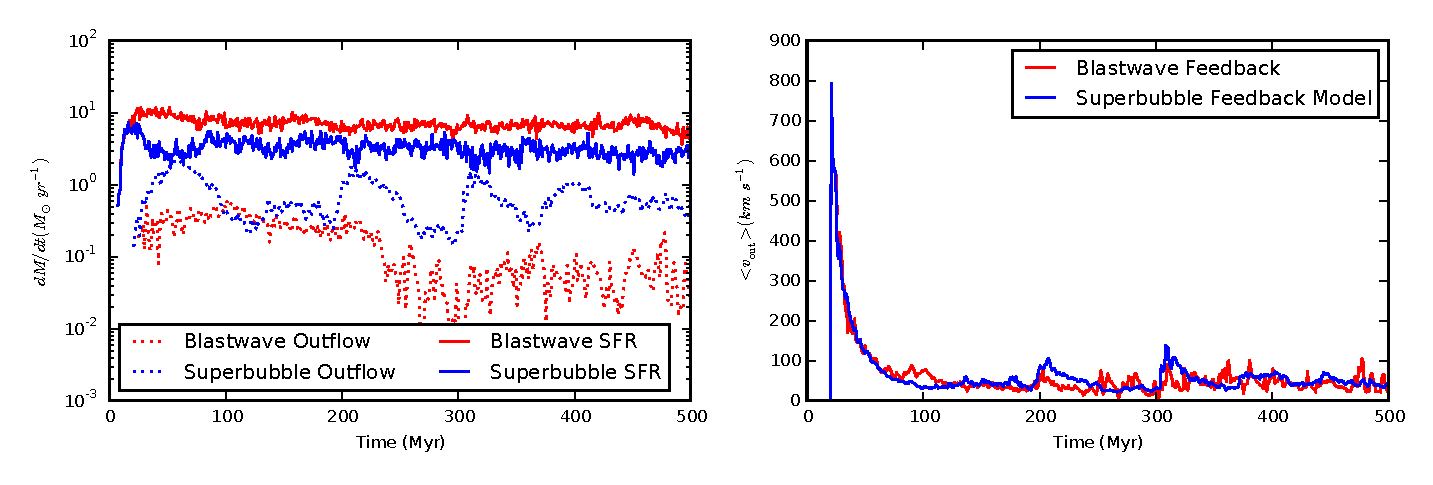
\includegraphics[width=\textwidth]{figures1/milkyway_outflow.eps}
    \caption[Outflow evolution in isolated Milky Way]{Outflow evolution for the
    Milky Way-like simulation.  The left hand plot shows the star formation rate
    and the outflow rate. The right hand plot shows the average outflow
    velocity.}
    \label{milkyway_outflow1}
\end{figure*}

\begin{figure*}
    \includegraphics[width=\textwidth]{figures1/dwarf_column.eps}
    \caption[Column density and temperature images of isolated dwarf]{Column
    Density (upper row) and temperature for the dwarf simulation at
    $300\;\mathrm{Myr}$.  The vectors in show the in-plane velocity.
    Temperatures shown are once again averages between the two phases for
    multiphase particles.  Note the much more `puffed up' appearance compared to
    the Milky Way, due to the more mass-loaded winds}
    \label{dwarf_column1}
\end{figure*}

\begin{figure*}
    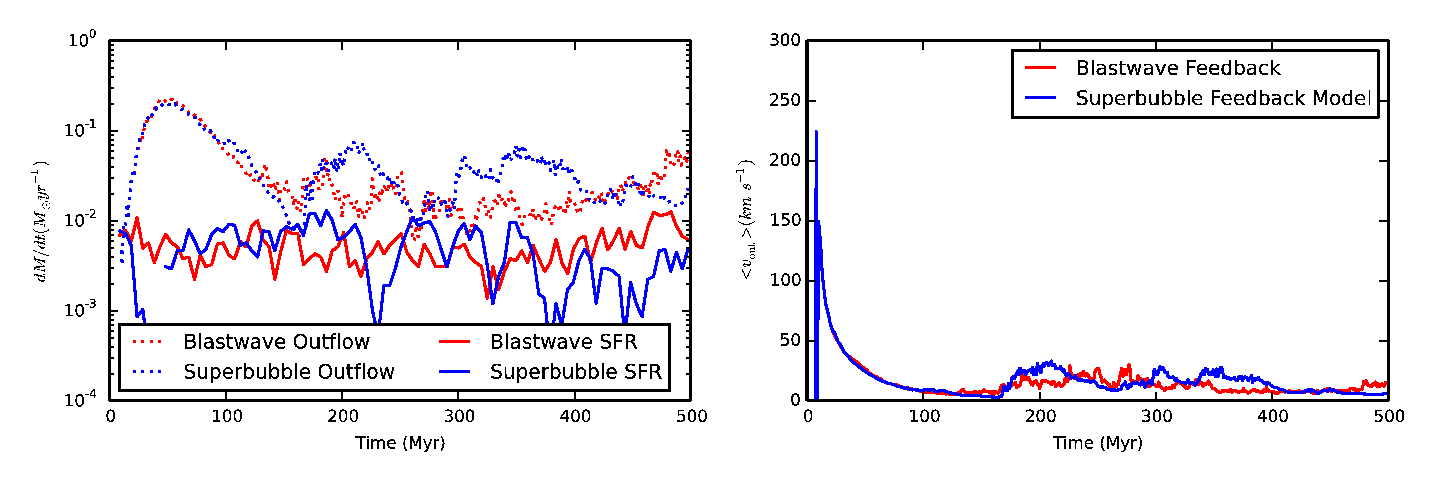
\includegraphics[width=\textwidth]{figures1/dwarf_outflow.eps}
    \caption[Outflow evolution in isolated dwarf]{Outflow evolution for the
    dwarf galaxy.  Note that the vertical ranges are different than in
    figure~\ref{milkyway_outflow1}}
    \label{dwarf_outflow1}
\end{figure*}

Figure~\ref{disc_phase1} shows phase diagrams from both Milky Way and dwarf
galaxies.  Figure~\ref{milkyway_column1} shows column density and temperature for
the Milky Way, and figure~\ref{milkyway_outflow1} shows star formation rates and
outflow properties.  Figures~\ref{dwarf_column1}~and~\ref{dwarf_outflow1} show the
same for the dwarf galaxy.  The Kennicutt-Schmidt relation for both galaxies is
shown in figure~\ref{kennicutt_schmidt1}.  The star formation and outflow properties are
discussed in section~\ref{Morphology1}.  Finally, we show some properties of the
multiphase particles in figure~\ref{multiphase_properties1}.

Figure~\ref{disc_phase1} shows that phase diagrams for galaxies using superbubble
feedback strongly distinguish between pre- and post-feedback gas.  Above $\sim
10^5\;\mathrm{K}$, we see (especially in the Milky Way), a hot medium of
including halo gas and low density gas inside superbubbles within the galaxy
disc (see the temperature slices in
figures~\ref{milkyway_column1}~and~\ref{dwarf_column1} for images of the gas
temperature in these bubbles).  The bulk of the gas lies at a roughly $10^4\;
\mathrm{K}$ equilibrium between cooling and photoheating from the UV background.
A cold medium of both dense shells surrounding superbubbles and cooling clouds
(soon to form stars) also forms in both the Milky Way and (to a lesser extent)
the dwarf.  The central panel shows a schematic of how gas migrates between
these regions.  Radiative cooling (blue arrow), bring gas to high densities.
Feedback creates a second hot phase in nearby gas particles.  The cold component
is relatively unaffected though it can compress due to the increased pressure
(staying near the tip of the blue arrow).  The hot and cold phases of multiphase
particles are plotted separately.  The hot component immediately moves to low
density and high temperatures,  $\gta 10^7$ K (the red arrow).  If the particle
continues to receive feedback, evaporation rapidly consumes its cold part and
the particle can flow out to the halo and remain buoyant and slow cooling.  It
evolves adiabatically as it does so (green arrow).

This panel is telling in that it shows that no gas is found within the
`forbidden' region of short cooling times of $\lta 10^4\;\mathrm{yr}$.
Cooling-shutoff methods often produce large quantities of this gas in a high
temperature, high density state.  If we were to simply take the average
temperature and density of the multiphase particles, they would almost entirely
lie within this region, on the line connecting the cold and hot phases (which,
of course, is exactly the impetus for using multiphase particles, since a
particle with the average properties would cool away all of its feedback energy
much too rapidly).

The roughly fixed amount of gas heated in the superbubble simulations shown
previously gives a roughly constant feedback-heated gas temperature of $\sim
2\times10^7\;\mathrm{K}$.  Figure~\ref{onestar_hottemp1}  shows that the actual
peak temperature of the feedback-heated bubble in the isolated star cluster run
varies between slightly less than this, to $\sim 1\times10^7\mathrm{K}$,
due to some cooling in the hot bubble.  This suggests that the model should
behave similarly to the stochastic thermal feedback model presented in
\citet{DallaVecchia2012}.  

As the multiphase fluid particles exist to bridge the gap between when the hot
interior of a superbubble contains too little mass to be resolved and the later
stage when resolved physics can take over, we should find that particles stay in
this phase for only a fraction of the lifetime of a superbubble.  From
\citet{MacLow1988}, the cooling time for superbubbles is on the order of a few
$10\;\mathrm{Myr}$, with a weak dependence on feedback luminosity and the
surrounding ISM density and metallicity.

We should expect that on average, multiphase particles convert back to single
phase in less than this time, a few $\mathrm{Myr}$.  In addition to their
lifetimes, we should expect multiphase particles to cluster in the discs of our
galaxy simulations (since they are spatially correlated with the stars that are
heating them), and that hot winds leaving the galaxy are composed of
fully-resolved, hot gas.  These winds are released when superbubbles grow large
enough to break out of the denser disc ISM, and thus should be well within the
resolved phase for these simulations.

Figure~\ref{multiphase_properties1} shows the duration that all particles stay in
the multiphase state as well as the maximum height reached by multiphase
particles.  The top figure shows that the vast majority of particles in either
the dwarf or the Milky Way convert back to single phase within
$10\;\mathrm{Myr}$.  The mean multiphase lifetime for the Milky Way was
$6.6\;\mathrm{Myr}$, and $2.7\;\mathrm{Myr}$ for the dwarf, well within the
range we should expect.  The reason for the shorter multiphase lifetimes in the
dwarf galaxy is simply the better mass resolution: the hot bubble interior
becomes resolved earlier in the dwarf than in the Milky Way.  Fewer than 0.5 per
cent of multiphase particles ever stay in the multiphase state for more than
$50\;\mathrm{Myr}$ in both the Milky Way and the dwarf.  The bottom figure
shows, again as we should expect, that most multiphase particles convert back to
single phase before they reach 1 scale height.  The mean maximum height for
multiphase particles was roughly $1/2$ a scale height for both simulations,
$0.51\;\mathrm{kpc}$ and $0.13\;\mathrm{kpc}$ for the Milky Way and dwarf
respectively.  Neither simulation had any multiphase particles reaching heights
of more than $10\;\mathrm{kpc}$ before converting back to single phase.  This
shows that multiphase particles are essentially embedded within the thin disc of
the ISM: all of the mass outflowing is fully-resolved hot gas, and its behaviour
is fully governed by standard hydrodynamics.  The winds driven from both
galaxies are ejected through nothing more than simple buoyancy.

\subsubsection{Galaxy Morphology and Outflows}\label{Morphology1}

\begin{figure}
    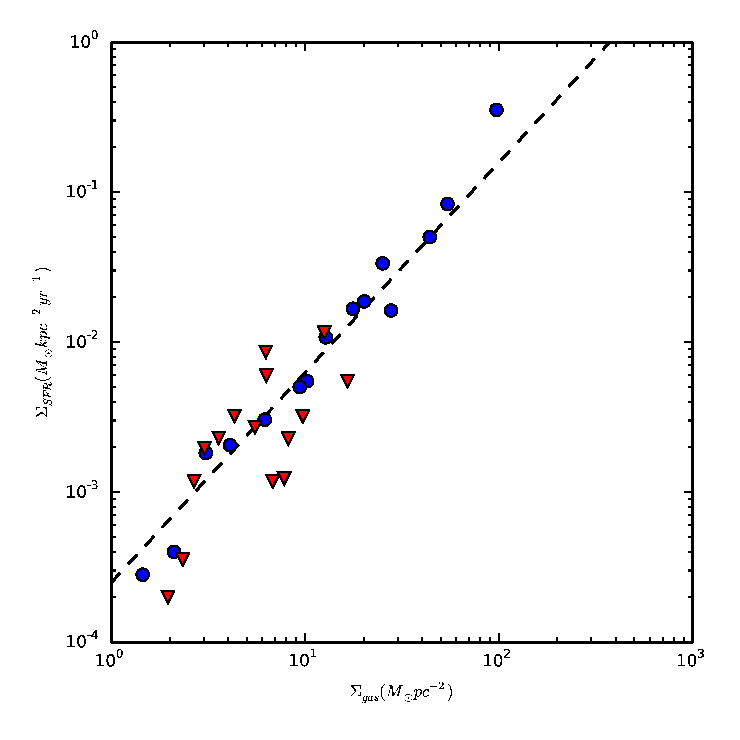
\includegraphics[width=0.6\textwidth]{figures1/kennicutt_schmidt.eps}
    \caption[Kennicutt-Schmidt law for isolated galaxies]{Kennicutt-Schmidt law
    in the Milky Way-like (blue points) and dwarf (red triangles) galaxies at
    $500\;\mathrm{Myr}$. Surface densities were calculated in radial annuli.
    The dashed line shows the Kennicutt-Schmidt Law.  The superbubble model is
    easily able to regulate star formation rates to within this range.}
    \label{kennicutt_schmidt1}
\end{figure}

\begin{figure}
    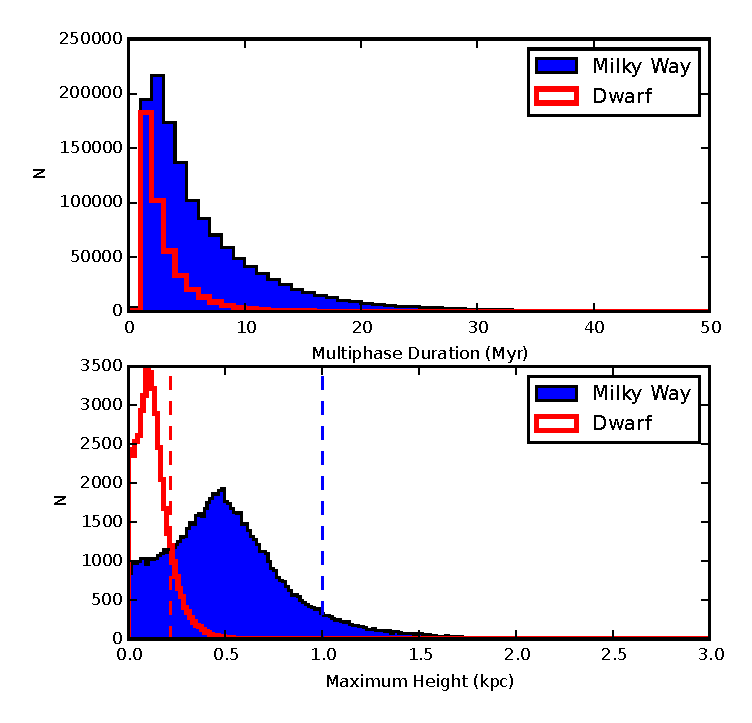
\includegraphics[width=0.6\textwidth]{figures1/multiphase_properties.eps}
    \caption[Properties of multiphase particles]{Properties of multiphase
    particles in the galaxy simulations.  The top figure shows duration of
    multiphase state for particles in both galaxy simulations.  Particles that
    are in the multiphase state more than once (convert back to single phase,
    cool, and then receive feedback again) have each time they are multiphase
    counted separately. The bottom figure shows maximum heights reached by
    particles in the multiphase state.  For each particle that is ever in the
    multiphase state, the maximum height it reaches {\it while still multiphase}
    is shown above for both galaxy simulations.  Dashed lines show scale heights
    at $10^4\;\mathrm{K}$ for each of the two simulations.}
    \label{multiphase_properties1}
\end{figure}
In order to compare superbubble feedback to \citet{DallaVecchia2012}, we selected
similar galaxies to the ones shown in their paper and calculated the properties
of their outflows using a similar method.  We adopt their two primary metrics,
mass outflow rate $\dot M$ and mean outflow velocity $<v_{\rm out}>$.  These two
metrics give us an idea as to both how much gas is ejected from the galaxies,
and how long that gas will take to return to the disc from the halo (if it does
return at all).

We calculated outflows from our galaxy simulations by selecting particles that
are moving away from the galaxy between a planar region 5 scale heights (5kpc
for the Milky Way, 1.13kpc for the dwarf) above and below the disc, and 0.5
scale heights thick.  The outflow rate $\dot M$ is simply the total momentum of
outflowing particles (particles returning on fountains are excluded) passing
through this region divided by the thickness of the region.  The average outflow
velocity $<v_{\rm out}>$ is just the mean velocity of these same particles.

The superbubble feedback method, as shown in figure~\ref{kennicutt_schmidt1} (and
the SFR shown in figures~\ref{milkyway_outflow1}~and~\ref{dwarf_outflow1}), also
passes the most basic requirement for a useful feedback model:  it is capable of
regulating star formation to match observed global star formation efficiencies.
This result is a typical outcome for effective feedback models with density-based 
star formation rates \citep[e.g.][]{Springel2003}.
Note that the simple star formation prescription used for
these tests does not have a cut-off at lower surface densities.  It is clear in
figure~\ref{milkyway_outflow1} that the average SFR in the Milky Way is roughly
twice as high in the simulation using blastwave feedback as compared to the
simulation with superbubble feedback.  It is also clear from this figure that
outflows in the Milky Way simulation with superbubble feedback contain
approximately ten times the mass of outflows driven by blastwave feedback.

\section{Discussion}

It is important to heat the right amount of gas through feedback. This is
particularly important if one wishes to examine feedback-driven galactic winds.
As figures~\ref{onestar_homogeneous1}~and~\ref{onestar_clumpy1} show, the simple
cooling-shutoff feedback model produces quite different amounts of hot gas as a
function of both resolution and ISM homogeneity.  If one underestimates the
amount of mass heated by feedback, the winds one drives will be hotter, but
contain less mass.  In other words, outflows will be faster but contain less
mass.  If one overestimates the amount of mass, outflows may carry a larger
fraction of the galaxy's gas mass, but will be less able to actually remove
this gas from the galaxy, either permanently or for a long cycling timescale.
Either error will have  serious implications for predictions of the effects of
outflows on both host galaxies and the intergalactic medium.  We have
constructed our model such that both the momentum and the amount of hot gas
within a superbubble are resolution independent.  This is confirmed in
figure~\ref{onestar_homogeneous1} over a range of mass 
resolutions from $\sim95M_\odot$ to $5\times10^4M_\odot$.  
Even in the extreme limit of a one particle superbubble,
the results are qualitatively correct and vary less than a factor of 2
from the expected solution.

In fact, for any feedback model that omits thermal conduction or other mixing
between the hot interior of a feedback bubble and the surrounding cold shell,
the amount of hot mass produced will be set by the resolution of the simulation
alone.  In fact, figure~\ref{onestar_homogeneous1} shows this quite clearly.  For
each resolution, the hot mass produced is roughly constant, simply a product of
the simulation mass resolution and the number of particles feedback is shared
with.  Changing either of these will drastically change the amount of hot gas
generated by feedback.  

In general, the gas driven in outflows from these galaxies does not move fast
enough to escape the galactic halos in either the dwarf and the Milky Way.  This
is reasonable for star formation rates well below the starburst regime.  The
majority of gas ejected from both simulations instead cycles between the halo
and the disc.  This helps moderate star formation in the disc.  By
$300\;\mathrm{Myr}$, only $\sim 1.0$ per cent, or roughly
$8.4\times10^7\;\mathrm{M_\odot}$, of the Milky Way gas has been lifted to above
5 scale heights while the dwarf cycles more than a third of its total gas mass,
$3.3\times10^7\; \mathrm{M_\odot}$ into a fountain above 5 scale heights.  In
both simulations, this cycling induces periodic bursts of star formation and
disc outflows.

As figures~\ref{milkyway_outflow1}~and~\ref{dwarf_outflow1} show, the superbubble
method results in galaxies with stronger star formation regulation, and
more mass-loaded outflows than the well-established blastwave model.  
For example, the simulation of the Milky Way analog, the star
formation rate is lower by a roughly a factor of 2 compared to the blastwave (a
point in favour of the superbubble model, since \citet{Scannapieco2012} showed
that a cosmological simulation of the Milky Way using blastwave feedback in
{\sc GASOLINE} formed stars at roughly twice the rates observed by
\citet{Guo2011}).  We also see roughly an order of magnitude more gas ejected
from the disc with the superbubble model, as we expect from the results of the
single star cluster test, since the production of more hot mass should result in
more mass-loaded winds.  Interestingly, the mean outflow velocity shows only
small differences between the superbubble and blastwave models.  This means that
even though the outflows driven by the blastwave contain less mass, they do not
leave the galaxy any faster, and are no more likely to escape the galactic
potential than winds produced in the superbubble simulations.

Our superbubble model is comparable to the model of \citet{DallaVecchia2012}
with a $\Delta T \sim 10^{7}\;\mathrm{K}$, somewhat smaller than their fiducial
value.  Both heat of order $300\;\mathrm{M_\odot}$ per SNe.
\citet{DallaVecchia2012} simply relied on a stochastic model to deposit enough
energy only when a specified temperature can be reached.   Their model suffers
from overcooling at cosmological resolutions with densities $n_H >
10\;\mathrm{cm^{-3}}$ as their stochastic model requires the heating of
fractional gas particles to yield the temperatures they desire.   At moderate
resolution, some star forming regions thus experience no feedback and others get
strong feedback.  The multiphase mechanism can handle resolutions where the
initial feedback-heated gas mass is less than a single resolution element,
without relying on stochastic feedback.

The superbubble method has a number of distinct advantages over previous feedback
methods (cooling shutoffs, constant-temperature stochastic feedback,
hydrodynamic decoupling, etc.).  The superbubble model introduces no additional
free parameters, requiring only the total stellar feedback energy to be
specified.  The superbubble paradigm can incorporate multiple sources of
mechanical luminosity, primarily stellar winds and supernovae, within a single
framework.  Unlike other methods, the amount of mass heated by feedback is
physically motivated: it is the amount of mass evaporated into the hot bubble
through thermal conduction.  Radiative cooling is suppressed not by simply
disabling it (which at best only approximates the long cooling times desired),
but by injecting energy into a distinct low density, hot phase.  This allows the
model to handle high-resolution isolated galaxy simulations as well as
lower-resolution cosmological ones.  

Another distinct advantage of this method is that it is {\it local}.
Feedback-heated gas needs no knowledge of its environment save the information
it has already through hydrodynamic interactions with its neighbours.  This
allows the method to handle feedback from clustered star formation without any
additional changes; gas particles need not know the {\it total} energy inside
a feedback-heated superbubble, which can be difficult to determine in a bubble
that is heated by multiple stars and contains many gas particles or cells.
Clustered star formation is an important aspect of galactic evolution, and can
amplify the effects of feedback by concentrating it on a single region
(something done by hand in stochastic, constant temperature feedback models).
As resolution in galaxy simulations has been steadily improving, well-resolved
clustered star formation is beginning to become a reasonable goal and object of
study.  The superbubble model will allow feedback from these clusters to behave
in a physically correct manner that is insensitive to resolution.

\subsection{Summary}
Stars preferentially form in clusters.  Clustered stellar feedback generates
superbubbles which are qualitatively different to isolated supernovae.
Correctly evolving superbubbles requires the inclusion of thermal conduction.
Thermal conduction, acting on very small length scales, evaporates cold material
into hot feedback bubbles which must be captured via a sub-grid evaporation
model such as the one presented here.  At the typical resolutions achievable in
galaxy simulations, a sub-grid multiphase treatment is required to accurately
follow the evolution of the hot phase.  Combining these elements results in a
feedback model with several attractive features:

\begin{enumerate}
    \item Separate hot and cold phases within an unresolved superbubble prevent overcooling
        without relying on ad-hoc cooling shutoffs
    \item Feedback from multiple sources (e.g. star clusters) is combined correctly
    \item Feedback gas doesn't unphysically persist in phases with extremely short cooling times
    \item Star formation is strongly regulated: at least as effectively as current models with the same
           feedback energy
    \item The feedback can effectively drive outflows
    \item Evaporation due to thermal conduction
        generates the correct amount of hot gas which 
        subsequently determines galactic wind mass-loading
    \item For well resolved bubbles, the model no longer relies on its multiphase component 
         and naturally produces superbubbles that behave as predicted
    \item The model is insensitive to resolution
\end{enumerate}

\section*{Acknowledgements}
The analysis was performed using the pynbody package \\
(\texttt{https://github.com/pynbody/pynbody}, \citep{pynbody})
  We thank Mordecai-Mark Mac Low for useful
conversations regarding this paper.  The simulations were performed on the
clusters hosted on {\sc sharcnet}, part of ComputeCanada.  We greatly
appreciate the contributions of these computing allocations. James Wadsley and
Hugh Couchman thank NSERC for funding support.
\bibliographystyle{mnras}
\bibliography{library}

\chapter{Cosmological Galaxy Evolution with Superbubble Feedback I: Realistic
Galaxies with Moderate Feedback}
\thispagestyle{fancy}
\textit{Reprinted from B.W. Keller, J. Wadsley, \& H.M.P.
Couchman 2015,} \\ \textsc{Montly Notices of the Royal Astronomical Society}
\textit{Volume 453, Issue 4, pp. 3499-3509, DOI: 10.1093/mnras/stv1789
Published by Oxford University Press on behalf of the Royal Astronomical
Society.  All rights reserved}
%\setcounter{pageFix}{\value{page}}
\begin{abstract}
\thispagestyle{fancy}
    \setcounter{page}{\value{pageFix}}
        \addcontentsline{toc}{section}{Abstract}
    We present the first cosmological galaxy evolved using the modern smoothed
    particle hydrodynamics (SPH) code \textsc{GASOLINE2} with superbubble
    feedback.  We show that superbubble-driven galactic outflows powered by Type
    II supernovae alone can produce $\rm{L^*}$ galaxies with flat rotation
    curves with circular velocities $\sim 200\; \rm{km/s}$, low bulge-to-disc
    ratios, and stellar mass fractions that match observed values from high
    redshift to the present.  These features are made possible by the high mass
    loadings generated by the evaporative growth of superbubbles.  Outflows are
    driven extremely effectively at high redshift, expelling gas at early times
    and preventing overproduction of stars before $z=2$.  Centrally
    concentrated gas in previous simulations has often lead to unrealistically
    high bulge to total ratios and strongly peaked rotation curves.  We show that
    supernova-powered superbubbles alone can produce galaxies that agree well
    with observed properties without the need for additional feedback mechanisms
    or increased feedback energy.   We present additional results arising from
    properly modelled hot feedback.
\end{abstract}

\section{Introduction}
The theory of galaxy formation is a cornerstone of modern cosmology.
$\rm{\Lambda CDM}$ accurately predicts the detailed properties of the Cosmic
Microwave Background, and the formation of large-scale cosmic structure.
Understanding how this yields the small-scale properties of the galaxies we see
today and at high redshift requires a good understanding of the
physics at play within these individual galaxies:  star formation, feedback, gas
accretion, etc.

The basic theoretical picture of galaxy formation is now well-established
\citep{Rees1977, White1978}.  The complex details are typically probed through
both simulation and semi-analytic techniques \citep{Kauffmann1999,Bower2006}.
Simulators typically employ large-scale cosmological boxes and zoomed in
simulations, in which regions sliced out of those larger volumes are re-simulated
at higher resolution \citep{Katz1993, Governato2004, Stinson2010, Brooks2011}.
Recent studies \citep{Dekel2006,Woods2014} have shown that the picture of how
gas is fed to galaxies is not simple:  cold flows can be funneled along
filaments in the cosmic web, bypassing the virial shock and directly supplying
gas to the inner galaxy.  Gas accretion and expulsion by stellar feedback is fundamental
to how galaxies evolve over time, determining not only when and how many stars
form, but the kinematic properties of those stars as well.

Stellar feedback has a greater impact than merely regulating star formation by
heating the ISM or increasing its turbulence.   It has long been understood that
the cumulative effects of multiple supernovae can eject gas from the galaxy,
powering a galactic outflow or wind \citep{Mathews1971,Larson1974}.  Galactic
winds are common in high-redshift galaxies, and can be seen in the nearby
Universe in starburst galaxies (See review by
\citealt{Veilleux2005}).  The detection of both blue-shifted rest-frame UV
absorption in observations of high redshift galaxies
\citep{Weiner2009,Steidel2010,Martin2012} along with broadened $H\alpha$
emission lines \citep{Heckman1987,Genzel2011,Newman2012} strongly suggests the
presence of hot, outflowing material surrounding these galaxies.  Galactic winds
appear to be ubiquitous at high-redshift, and are likely a key factor in the
evolution of galaxies in the early Universe.  \citet{Muratov2015} estimated that
mass loadings for winds peaked at roughly $\eta=\frac{\dot M_{wind}}{\dot
M_{*}}\sim10$ at high redshift and that a significant
fraction of ejected material can escape beyond the virial radius.  By ejecting
material from a galaxy's disc, and storing it in the hot, gravitationally bound
circumgalactic medium (CGM), star formation at high redshift can be strongly
regulated, while at the same time providing a reservoir of gas that can be
accreted at late times, ensuring that star formation at low redshift can
continue \citep{Marasco2012}.  How this CGM is created is complex, as it is
potentially pierced by cold flows of infalling material, outflows from the
central galaxy, and the accretion of dwarf satellites.

The first generations of cosmological simulations including baryonic physics
(hydrodynamics, star formation, etc.) suffered from a number of serious
problems.  Nearly every simulation, regardless of halo mass, produced far too
many stars, and tended to form these stars too early \citep{Abadi2003,
Governato2009, Stinson2010, Brooks2011}.  Simulations of disc galaxies produced
bulge dominated galaxies rather than the thin discs we observe.  Together with
the discrepancies seen between large dark-matter only simulations and
observations, it appeared that the standard dark energy + cold dark matter
cosmology $\rm{\Lambda CDM}$ might need to be modified to adequately explain the
properties of both individuals galaxies and populations of galaxies that we see.
\cite{Scannapieco2012} showed these problems were ubiquitous among codes,
leading simulators to consider a role for stronger feedback.  Early feedback
models (e.g. \citealt{Katz1993}) tended to deposit the energy of feedback into a
poorly-resolved region of the interstellar medium, subjecting it to
over-cooling.  Stronger feedback can be achieved by limiting cooling or
increasing the total energy.  It must also ensure that feedback energy couples
strongly to the gas.  This strong coupling doesn't just heat the ISM, or disrupt
only the densest regions, but drives outflows that actively remove gas from the
disc of the galaxy.   The Aquila comparison of 13 different simulation codes and
subgrid physics models \citep{Scannapieco2012} showed that only those cases with
strong outflows could produce galaxies with realistic star formation histories.
The outflow models used were somewhat ad hoc and extremely aggressive.  The
cases that were capable of ejecting sufficient gas from the galaxy disc to
moderate the stellar mass of the halo still failed to produce stellar discs and
largely shut down low redshift star formation.

Galactic winds have been a part of cosmological galaxy simulations for 
some time \citep{Springel2003}, and recent simulations have investigated these
winds in detail.    \citet{AnglesAlcazar2014} showed that these winds can dramatically
alter the star formation history, kinematics, and morphology of galaxies at
redshift 2.  By explicitly creating galactic winds with a variety of
mass-loadings and wind velocities, they showed that strong winds are essential
to producing the gas-rich, extended, and turbulent discs that are typically
observed in high redshift star forming galaxies.  Unfortunately, without 
simulations to $z=0$, interpreting exactly how these high-redshift winds impact
present-day galaxies is difficult. If outflowing material falls back onto the
galactic disc within a Hubble time, the effects of high-redshift winds may be
seen in the form of increased star formation and inflows at low redshift.  

A key question remains: What processes set the mass loading and velocity of
these winds?  Early work tied galactic outflows to the SNe energy
\citep{Springel2003}.  Some studies (e.g. \citealt{Murray2005,Krumholz2013})
have suggested that radiation pressure is needed to drive sufficient
galaxy-scale winds.  Others argue that galactic winds could be powered by cosmic
ray buoyancy \citep{Ipavich1975,Breitschwerdt1991,Socrates2008}.

Today, multiple different models of strong feedback have begun to produce
galaxies with the correct number of stars \citep{Aumer2013}, reasonable star
formation histories \citep{Stinson2013,Agertz2015,Munshi2013}, and correct
morphologies \citep{Guedes2011,Brook2012,Christensen2014}.   Unfortunately, many
of these successes have come at the cost of increasing complexity in star
formation and feedback methods, crude assumptions regarding the physics of the
feedback-heated gas and somewhat arbitrary increases in the feedback energy per
unit mass in stars.  

In many cases, strong feedback simply means more energy.  Many modern feedback
models augment the energy input from Type II supernovae ($\sim10^{51}\;
\rm{erg}$ per star above $8\; \rm{M_\odot}$), with that arising from stellar
winds, UV ionization, supermassive black holes (SMBH), or radiation pressure
\citep{Vogelsberger2013, Agertz2015}.  Feedback models such as
\citet{Stinson2013} group these sources of energy as early stellar feedback.
Since the first supernovae occur $\sim4\; \rm{Myr}$ after star formation, these
feedback mechanisms begin depositing feedback before SN-only methods would.
Unfortunately, how much energy from these early feedback effects actually
couples to the surrounding ISM rather than radiating away is highly uncertain.
In fact, even the coupling of comparatively simpler SN feedback still is a
matter of some debate.  Many new feedback models \citep{Agertz2013, Aumer2013,
Hopkins2013} treat each of these feedback mechanisms explicitly, modelling the
input of energy and momentum from each component separately.  

In addition to increasing the total amount of energy deposited by stellar
feedback, these models often also include components designed to prevent energy
from feedback radiating away (a problem discussed thoroughly in
\citealt{Thacker2000}).   The energy can be prevented from cooling completely
for a while \citep{Stinson2013} or it can be initially placed into a non-cooling
reservoir that leaks back into regular thermal energy \citep{Agertz2013}.
Alternately, depositing thermal feedback into a sufficiently small mass, allows
it to always heat gas to the same high temperature where cooling times are long
\citep{DallaVecchia2012}.  Depositing feedback as kinetic avoids initial
radiative losses \citet{Springel2003,Agertz2013,Hopkins2013}.  

While these techniques do help solve the overcooling problem, they all come with
some drawbacks.  Fixed-temperature thermal feedback is stochastic, and requires
the additional free parameter of the feedback temperature. Cooling shutoffs
completely disable radiative losses, where in nature these losses are suppressed
in some regions but can remain strong in others, depending on the structure of
the ISM and the clustering of stars.  Kinetic feedback is almost always paired
with a temporary decoupling of hydrodynamic forces on feedback-accelerated gas.
This is necessary to prevent this gas from shock-heating and potentially
reintroducing the overcooling problem (as shown by
\citealt{Creasey2011,Durier2012}).  Decoupling allows winds to escape.  However,
this makes it impossible to study the detailed behavior of these winds, and how
they interact with the ISM.  This makes the mass loading an imposed parameter.

Of these methods, \citet{DallaVecchia2012} showed the interesting result that,
for supernovae alone, depositing feedback energy into a pre-specified amount of
mass, without any cooling shutoffs, can give reasonable star formation rates and
strong galactic outflows in isolated galaxies.  \citet{Keller2014} argued that
what sets this mass is thermal conduction in superbubbles, and used that
mechanism to build a new way of simulating supernovae feedback that lacked the
resolution dependence, additional complexity, and ad-hoc additions of many
current feedback models.  By focusing on superbubbles, and the evaporation of
cold gas to determine mass loading, superbubble feedback gives realistic gas
behavior, and is effective at both regulating star formation and driving
galactic outflows without introducing free parameters.

The original McMaster Unbiased Galaxy Simulations (MUGS; \citealt{Stinson2010})
showed that with stellar feedback, the observed color-magnitude relationship and
Tully-Fisher relation could be produced in simulated $\rm{L^*}$ galaxies.  It
failed, however, to produce galaxies with the correct stellar mass fraction and
star formation history, overproducing stars over the entire cosmic history, and
grossly overproducing them at high redshift.  It also produced galaxies with
bulge-to-disc fractions larger than those seen in nature, and with sharply
peaked rotation curves.  \citet{Stinson2013} showed that the addition of early
stellar feedback could alleviate most of these problems.  That model does not
take into account the potentially complex coupling of stellar winds or radiation
pressure to the surrounding ISM.  Instead, a substantial (fixed) fraction of the
stellar bolometric luminosity was applied as feedback heating.

In this paper, we begin first with an overview of the simulation methods used,
both gas microphysics and the star formation and feedback techniques.  We then
present the results of a suite of 4 simulations using an initial
condition from the MUGS sample, each generated with different stellar feedback
models or energetics.  The resulting galaxy properties,  as well as the halo
evolution are examined over the lifetime of the galaxy.  Finally, we discuss how
the superbubble-driven outflows change with time, and how they ultimately result
in a realistic galaxy at the present epoch.

\section{Methods}

These simulations were run using a modern update to the SPH code {\sc GASOLINE}
\citep{Wadsley2004}, {\sc GASOLINE2}.  The changes in this new code include a
sub-grid model for turbulent mixing of metals and energy \citep{Shen2010}, and a
modified pressure force form similar to that proposed by \citet{Ritchie2001}
which is functionally equivalent to \cite{Hopkins2013}.  These changes solve the
problems seen in Kelvin-Helmholtz and blob destruction tests with SPH
\citep{Agertz2007}.  These and other features are discussed in
\citet{Keller2014}.  Accurately modelling mixing in multiphase gas is essential
for accurately simulating the ISM and CGM.

\subsection{Simulations}
For this initial study, we have selected the initial conditions from one of the
original MUGS galaxies. We selected an intermediate-mass halo, g1536, allowing
us to compare to a number of other studies that have examined this particular
halo (e.g. \citealt{Stinson2013,Woods2014}).  At $z=0$ this halo has a virial
mass of $8\times10^{11}\; \rm{M_\odot}$ and a spin parameter of 0.017.  It had
its last major merger at $z=2.9$.  We have a gas mass resolution of
$M_{gas}=2.2\times10^5\; \rm{M_{\odot}}$, and use a gravitational softening
length of $\epsilon=312.5\; \rm{pc}$.  The details of how this IC was created
can be found in \citet{Stinson2010}.  We choose to focus on a single galaxy for
this paper as it allows us to make a direct comparison of the impact feedback
physics makes with relatively little expense.  Naturally, this limits our
ability to comment on population-wide effects.  We leave this discussion
for a forthcoming paper in which we introduce 17 additional $L^*$ galaxies.

We compare four test cases using the same initial conditions: no stellar
feedback (an absolute lower bound for looking at the effects of feedback);
superbubble feedback (our fiducial case); blastwave feedback (the feedback
method used in \citet{Stinson2010}, first described in \citealt{Stinson2006}); and
superbubble feedback with double the standard feedback energy ($2\times10^{51}\;
\rm{erg}$ per SN).  The high feedback energy case uses more feedback than is
predicted by \citet{Leitherer1999}, but is within the range of feedback energies
currently being used in cosmological simulations \citep{Schaye2015, Agertz2015,
Vogelsberger2013}.  

Halos were found in each of the simulations using the Amiga Halo Finder
\citep[AHF;][]{Knollmann2009}.

\subsection{Star Formation and Feedback}
Our suite of simulations use a range of different feedback
processes.  For all of the simulations shown in this paper, we use a common
star formation prescription.  Stars are formed at a rate proportional to the
local free-fall time of gas, such that
\begin{equation}
    \dot \rho_* = c_* \frac{\rho_{gas}}{t_{ff}}
    \label{sflaw}
\end{equation}
For each of these simulations, we used an efficiency parameter $c_* = 0.1$, the
value used by \citet{Stinson2013}.  Stars are allowed to form in a converging
flow when gas is cooler than $1.5\times10^4\; \rm{K}$, and with a density set to
that allowed by the gravity resolution, $\rho = M_{gas}/\epsilon^3 = 9.3\;
\rm{cm^{-3}}$.

The amount of supernova feedback per unit stellar mass is determined using a
\citet{Chabrier2003} IMF.  With $\sim10^{51}\; \rm{erg}$ per supernova this
gives $\sim10^{49}\; \rm{erg\;M^{-1}_{\odot}}$.   A notable difference between
this simulation and those of \citet{Stinson2013} and others is that we do not
include early feedback, processes such as stellar winds and radiation that can
inject energy before supernovae occur $\sim 4\; \rm{Myr}$ after the first
massive stars form.  A primary role for early stellar feedback is to disrupt the
densest molecular gas.  In these simulations, this dense molecular gas cannot be
resolved, never being formed (and thus it does not form or need to be
destroyed).

The feedback recipe used in our main simulations is the superbubble method
presented in \citet{Keller2014}.  This method deposits feedback into resolution
elements in a brief multi-phase state.  These particles each have separate
specific energies, masses and densities, for the hot bubble and surrounding cold
ISM, which includes the swept up shell.  This allows the method to calculate a
separate density and cooling time with the respective densities for each phase,
rather than the average density of both phases.  Multiphase particles are also
prevented from forming stars: the average temperature of the two phases is
essentially always above our temperature threshold for star formation.  More
details on this method can be found in \citet{Keller2014}.

The addition of thermal conduction and evaporation introduces some additional
time step constraints in order to ensure the stability of integration.  However,
since the thermal conduction rate is capped by the saturation imposed by the
electron soundspeed, this time step is at worst 1/17 the Courant time step. In
fact, we see an overall speedup when using superbubble vs. blastwave feedback,
as gas can no longer exist in the regime of high density and temperature (and
thus small Courant times).  The average computation time per step was $\sim
25\%$ faster using superbubble feedback compared to blastwave feedback.  These
benefits are dominant late in the run, as the total amount of dense gas becomes
larger. We do see some slight increased cost early in the run, with a slowdown
of $\sim50\%$ before z=4.  The additional time-step constraints here are similar
to the time-step constraints required for other methods as well, such as
decoupled kinetic winds \citep{Springel2003}.


\subsection{Gas Cooling and Physics}
We adopt the same gas cooling physics as a number of past simulations using
\textsc{GASOLINE} \citep{Stinson2013,Keller2014}.  The method for cooling we use
here was originally presented in \citet{Shen2010}.  Our simulations use cooling
rates from \textsc{CLOUDY} \citep{Ferland2013}, and  include a
redshift-dependent UV background, Compton cooling, and primordial and metal
cooling from 10 to $10^9\; \rm{K}$.  This sets these simulations apart from many
past simulations \citep{Governato2009,Brook2011,Guedes2011}, which did not
include high temperature metal cooling.  We impose an artificial pressure floor,
using a method described by \citet{Robertson2008} to prevent spurious Jeans
fragmentation (as cold, dense gas has both Jeans length and Jeans mass below the
resolution limit of our simulation).  We also enforce that the minimum SPH
smoothing length a particle may have is $\epsilon/4$.  This is equivalent to a
density floor of $400\; \rm{cm^{-3}}$ (note that for two-phase superbubble
particles, this is the maximum \textit{mean} density).  These are comparable to
the parameter choices in another recent re-simulation of the MUGS initial
conditions, \citet{Stinson2013}.

\begin{figure}
    
    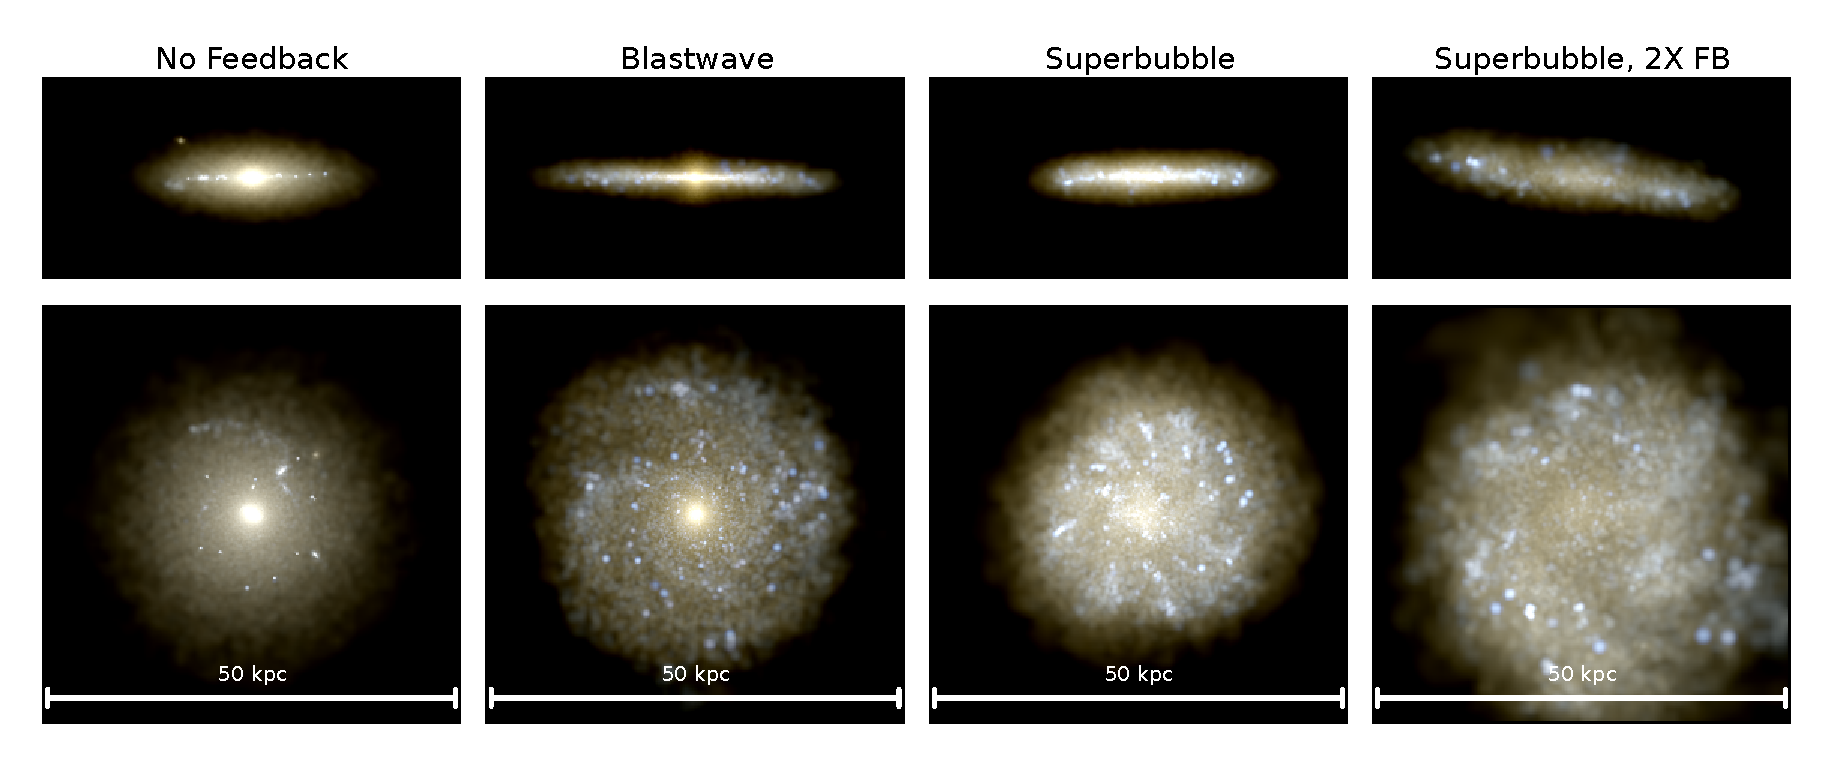
\includegraphics[width=\textwidth]{figures2/stellar_image.eps}
    \caption[Mock stellar image of galaxy at z=0 with different feedback
    models]{Mock stellar image of each galaxy at $z=0$.  The top row shows the
    galaxies edge-on, while the bottom shows them face-on.  The no-feedback case
    shows very little disc, while the blastwave feedback case has a thin disc
    with a prominent bulge.  The superbubble galaxy appears nearly bulgeless,
    composed only of a truncated disc. Note also that the superbubble galaxy is
    bluer than the blastwave or no-feedback galaxies, evidence of a younger
    stellar population.}
    \label{stellar_image}
\end{figure}
\begin{figure}
    \includegraphics[width=\textwidth]{figures2/column_density.eps}
    \caption[HI column density in a galaxy at z=0 with different feedback models]{HI
    column density for the four test cases at z=0.  The no feedback case has
    exhausted nearly all of the gas within the disc, leaving only diffuse wisps.
    The two superbubble cases (especially with doubled supernova energy) have
    lofted a large amount of gas out of the disc, and some entrained dense
    clumps can be seen in this outflowing material.  The superbubble gas discs
    are much more flocculent than the blastwave disc, and where the feedback
    energy is doubled, the disc is strongly disrupted.}
    \label{column_density}
\end{figure}
\begin{figure}
    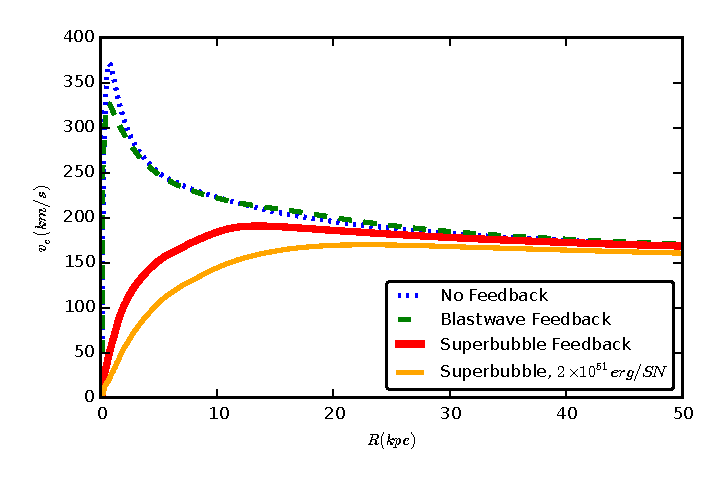
\includegraphics[width=0.6\textwidth]{figures2/rotation_curve.eps}
    \caption[Rotation curves with different feedback models]{Rotation curves for
    each of our test cases.  As is clear, the superbubble cases have much lower
    central concentrations, giving a a rotation curve that rises to a flat
    $200\; \rm{km/s}$.  The peaked rotation curves in the cases with blastwave
    or no feedback are a result of their failure to remove low angular momentum
    gas at high redshift, giving bulge-dominated, centrally concentrated
    galaxies.}
    \label{rotation_curve}
\end{figure}

\section{Results}
\subsection{Redshift zero Disc Properties}
\begin{table}
    \scriptsize
    \begin{tabular}{ c c c c c c c}
        \hline
        Simulation & $M_{vir}$ & $M_{gas}$ &
        $M_{star}$  &$M_{bary,0.1vir}$ & $M_{bulge}$ & $M_{disc}$ \\
        \hline
        No Feedback & $7.94\times10^{11}$ & $6.21\times10^{10}$ &
        $7.42\times10^{10}$ & $8.09\times10^{10}$ & $9.34\times10^{9}$ &
        $2.88\times10^{10}$\\
        Blastwave Feedback & $7.99\times10^{11}$ & $8.05\times10^{10}$ &
        $5.11\times10^{10}$ & $7.94\times10^{10}$ & $8.09\times10^{9}$ &
        $1.75\times10^{10}$ \\
        Superbubble Feedback & $8.02\times10^{11}$ & $1.19\times10^{11}$ &
        $1.84\times10^{10}$ & $6.25\times10^{10}$ & $1.14\times10^{9}$ &
        $1.15\times10^{10}$ \\
        Superbubble, $2\times10^{51} erg/SN$ & $7.96\times10^{11}$ &
        $1.20\times10^{11}$ & $1.09\times10^{10}$ &  $4.92\times10^{10}$ & 
        $5.96\times10^{8}$ & $6.98\times10^9$\\
    \end{tabular}
    \caption[Halo Components at $z=0$ for different feedback models]{Halo
    components at $z=0$. $M_{disc}$ and $M_{bulge}$ are the determined by the
    angular momentum of the stars (as detailed below).  All masses are in
    $M_\odot$.}
    \label{properties}
\end{table}

As can be seen in Figure~\ref{stellar_image}, the galaxy produced with
superbubble feedback is disc-dominated and blue.  The stellar disc in the case
without feedback is nearly non-existent, with an ellipsoidal morphology.  The
superbubble disc appears somewhat thicker and truncated compared to the disc
produced with blastwave feedback.  The truncation can be seen in the reduced
stellar scale length of the superbubble galaxy, $2.9\;\rm{kpc}$ vs.
$3.8\;\rm{kpc}$ for the superbubble vs. blastwave galaxies.  The thickening
appears to be quantitatively insignificant, however, as both discs have stellar
scale heights of $0.9\;\rm{kpc}$ This may be due to the the disc being disrupted
at large radii, where the surface densities are lower, allowing superbubbles to
grow larger and escape more easily.  The increased feedback case is
interestingly somewhat tilted compared to the rotation of the halo as a whole.  
\begin{figure}
    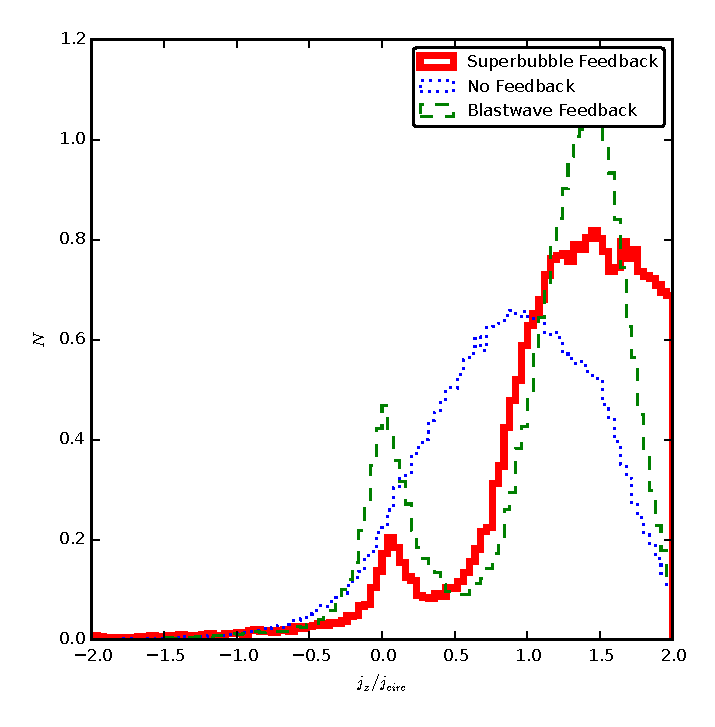
\includegraphics[width=0.6\textwidth]{figures2/circularity.eps}
    \caption[Stellar orbit circularity histogram]{Histogram
    of stellar orbit circularity.  The bimodal distribution shows the bulge
    component, with a circularity near 0, and the disc component, with a
    circularity near 1.  Note that without feedback, this bimodality disappears,
    as the galaxy morphology becomes spheroidal.  The values here are normalized
    so that each curve has a total integral of unity.  As is clear, very few
    stars produced in a galaxy with superbubble feedback have low angular
    momentum, giving us a disc-dominated galaxy.}
    \label{circularity}
\end{figure}
\begin{figure}
    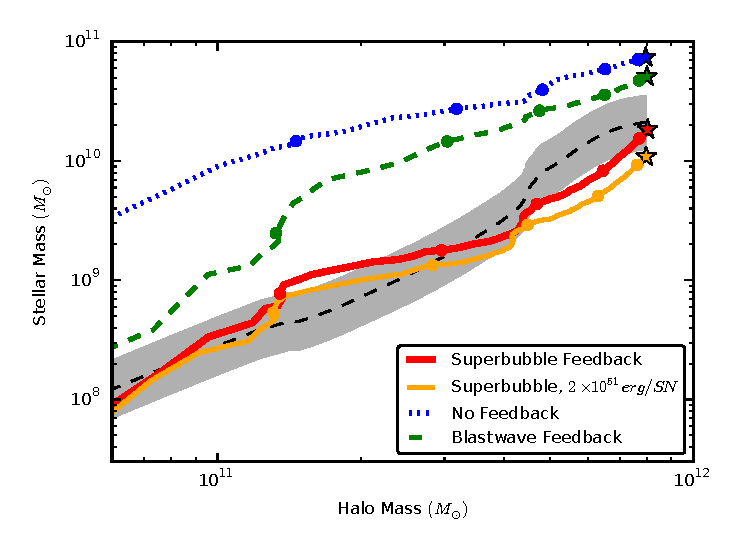
\includegraphics[width=0.6\textwidth]{figures2/mass_growth.eps}
    \caption[Stellar mass growth for different feedback models]{Stellar mass
    growth as a function of the total halo mass.  The grey band and black dashed
    curve show mean values and uncertainties from the abundance matching results
    of \citet{Behroozi2013}.  The points show values at redshifts 3,2,1,0.5, and
    0.1.  The stars show the final values at redshift 0.  For essentially the
    entire evolution of the halo, both the no feedback galaxy and the blastwave
    galaxy overproduce stars.}
    \label{mass_growth}
\end{figure}
\begin{figure}
    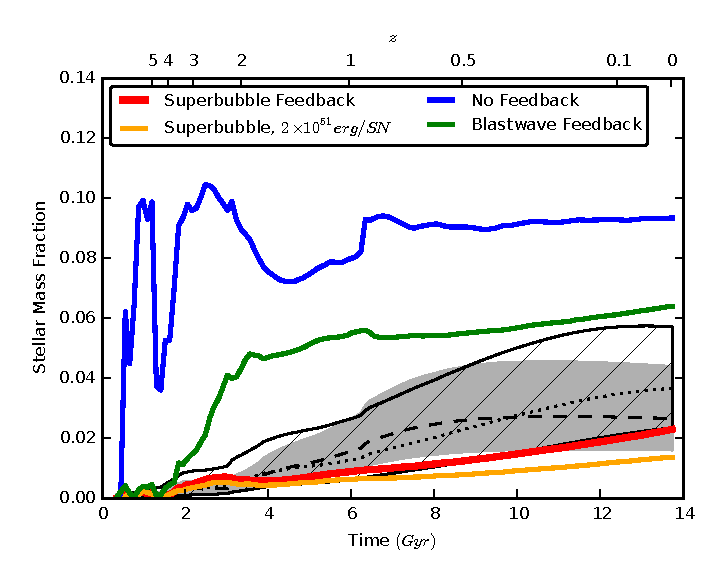
\includegraphics[width=0.6\textwidth]{figures2/stellar_fraction.eps}
    \caption[Stellar mass fraction evolution]{Stellar mass fraction as a
    function of time/redshift.  As in figure~\ref{mass_growth}, only the
    fiducial superbubble run produces stellar mass fractions within observed
    uncertainties for the entire history of the halo. The grey band is as in
    figure~\ref{mass_growth}, and here we also show, in the hatched region with
    the dotted curve, values and uncertainties from \citet{Moster2013}.  The dip
    that can be observed in the no feedback case at high redshift come from the
    growth of the halo, as it accretes dark matter dominated dwarves.}
    \label{stellar_fraction}
\end{figure}
\begin{figure}
    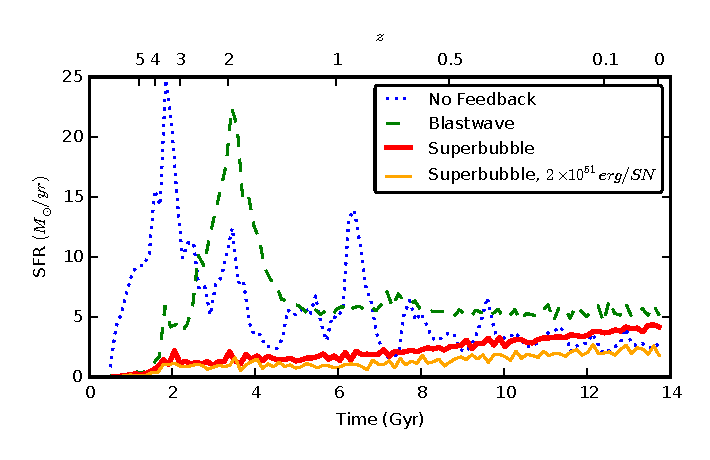
\includegraphics[width=0.6\textwidth]{figures2/sfr.eps}
    \caption[Star formation rate as a function of feedback model]{Star formation
    rates for all 4 simulations.  The low star formation rate seen after $z=1$
    in the no feedback case is due simply to the high z star formation consuming
    most of the available gas.}
    \label{sfr}
\end{figure}
\begin{figure}
    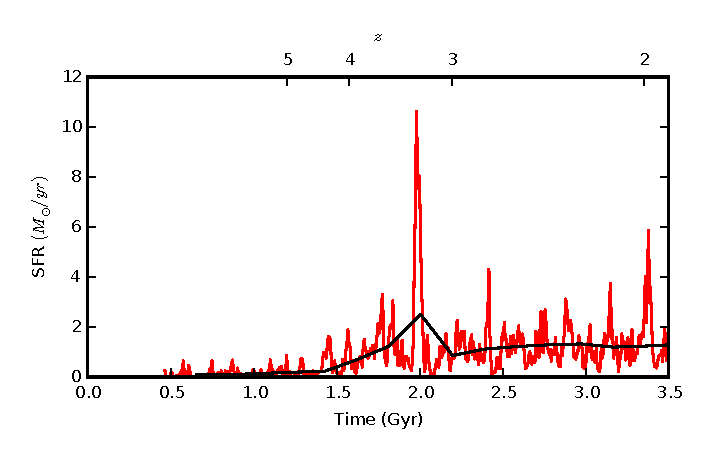
\includegraphics[width=0.6\textwidth]{figures2/burstiness.eps}
    \caption[Superbubble star formation burstiness]{Star formation rate up to
    $z=2$ for our superbubble galaxy.  As is clear, when sampled on short ($7\;
    \rm{Myr}$) timescales, the star formation rate in the superbubble galaxy is
    characterized by strong bursts, despite its quiescent behavior averaged over
    longer timescales.}
    \label{burstiness}
\end{figure}
\begin{figure}
    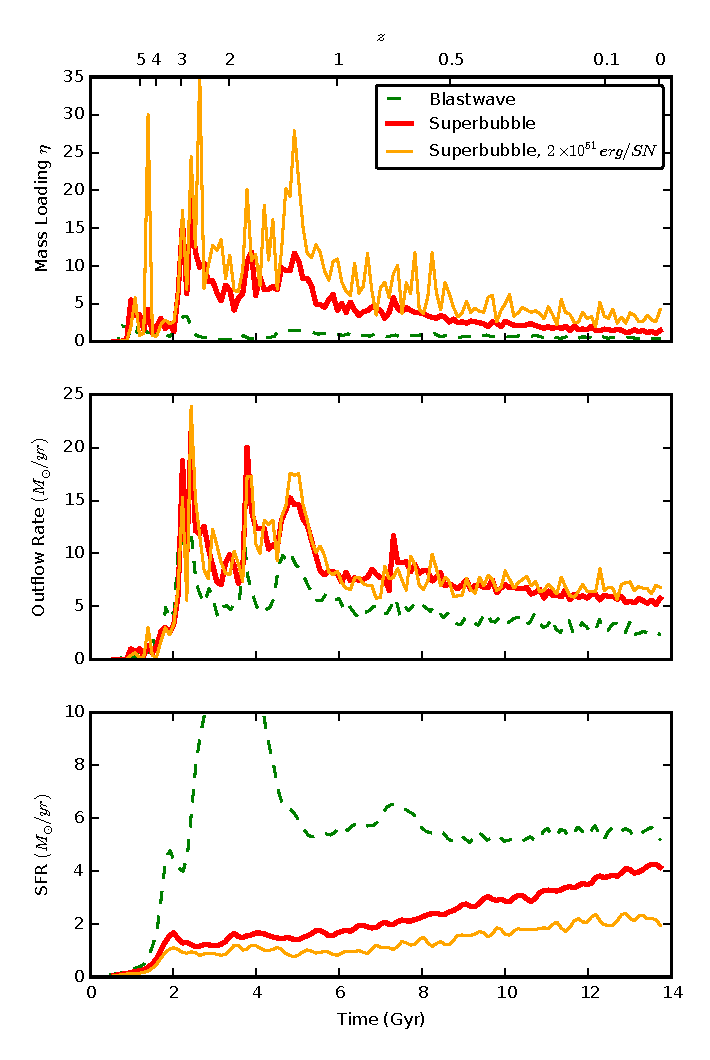
\includegraphics[width=0.8\textwidth]{figures2/massloading.eps}
    \caption[Galactic wind mass loading for different feedback models]{Galactic
    wind mass-loading and outflow rates for each feedback model.  As is clear,
    superbubble feedback powers winds with significantly higher mass-loadings,
    and, despite forming less than half as many stars the blastwave galaxy,
    results in more total outflowing gas.  This is key to the regulatory power
    of superbubbles.  Despite the peak in outflow rate in the blastwave case
    between $z=4-1.5$, the massively increased star formation rate seen in the
    the smoothed SFR during this time (bottom plot) means that the mass-loadings
    never go above 5, and baryon expulsion is inefficient.}
    \label{massloading}
\end{figure}

The gas component of this galaxy can be seen in Figure~\ref{column_density}.
The superbubble feedback is clearly much more effective at ejecting gas from the
disc, creating a halo of clumpy HI gas.  In the doubled feedback case, the disc
is heavily disrupted, with no spiral structure visible in either the stellar or
gas density images.  Thus the larger stellar disc is directly related to a more
extended gaseous disk.

The rotation curve in Figure~\ref{rotation_curve} shows that this ejection also
gives a flattened rotation curve without the central peak seen in simulations
with blastwave or no feedback.  This tells us that the mass distribution is much
less centrally concentrated when superbubble feedback is used, more evidence
that superbubble feedback is effective in preventing bulge formation.

One of the primary problems in older simulations was a much larger
bulge-to-total fraction based on a kinematic decomposition.  We adopt the same
kinematic decomposition as the original MUGS study.  We calculate, for each star
within the halo, a circularity parameter, which is simply the ratio of the
specific angular momentum component perpendicular to the disc ($j_z$) and the
specific angular momentum for a perfect circular orbit in the same potential
that the star sees $j_{circ}$.  As in the original MUGS study, we identify bulge
stars as having $j_z/j_{circ} < 0.7$ and orbital radii of $< 5\; \rm{kpc}$.  We
find, using these criteria, that our fiducial B/T ratio at $z=0$ is 0.09,
slightly smaller than the Milky Way's $\sim0.14$, and greatly reduced compared
to the 0.55 found in the original MUGS paper, and well within the observational
constraints from \citet{Allen2006}.  As these numbers, and the distribution of
this circularity parameter found in Figure~\ref{circularity} show, the vigorous
expulsion of central gas with superbubble feedback is a powerful bulge
prevention and destruction mechanism.  Each of the 13 samples from the Aquila
project \citep{Scannapieco2012} suffered from either from a bulge-dominated
stellar circularity profile, or from a massively peaked (or in some cases simply
too high) rotation curve.  Even the three cases that managed to produce a
reasonable stellar mass fraction (each of these generated strong outflows,
either through SMBH feedback or wind decoupling) still failed to produce
disc-dominated galaxies.  Of their sample, only four cases had more than 40\% of
the stellar mass in disc stars, but all of these cases massively overproduced
stars.

The ejection of gas is evident if we look at the baryon content of the interior
part of the halo, where the disc resides, in this case, simply material within
$0.1R_{vir}$,.  With superbubble feedback, the baryon fraction of this inner
region is 0.30, reduced from 0.37 without feedback, and 0.35 with blastwave
feedback.  This means that nearly 20\% of the baryons that would be available to
form stars have been blown out of the galaxy disc, roughly twice the amount that
was removed by the older feedback model.  The baryon deficit in the superbubble
is comparable to the total stellar mass of the galaxy (the fiducial case has a
$1.5\times 10^{10}M_\odot$ deficit in baryons (compared to the no-feedback
case), and a total stellar mass of $1.8\times 10^{10}M_\odot$).  

Of what remain, only 29\% of the baryonic mass in the superbubble galaxy disc is
in stars, compared to 63\% in the blastwave galaxy, and 89\% in the no
feedback galaxy.  The basic properties of each halo can be found in
table~\ref{properties}.

\subsection{Halo Evolution and Star Formation}
\begin{figure}
    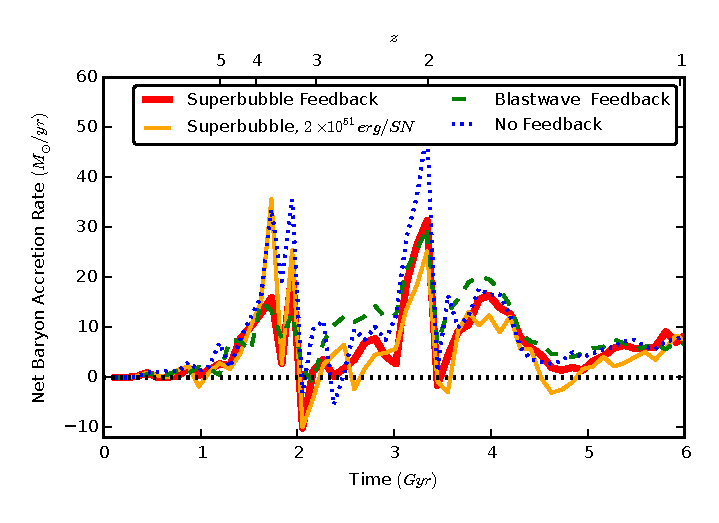
\includegraphics[width=0.7\textwidth]{figures2/net_accretion.eps}
    \caption[Net baryonic accretion for different feedback models]{Net baryonic
    accretion (stars and gas) for each test case.  It is clear that superbubble
    feedback expels baryons much more effectively than the blastwave feedback
    model (although even weak feedback does help somewhat compared to no
    feedback whatsoever).}
    \label{net_accretion}
\end{figure}
\begin{figure}
    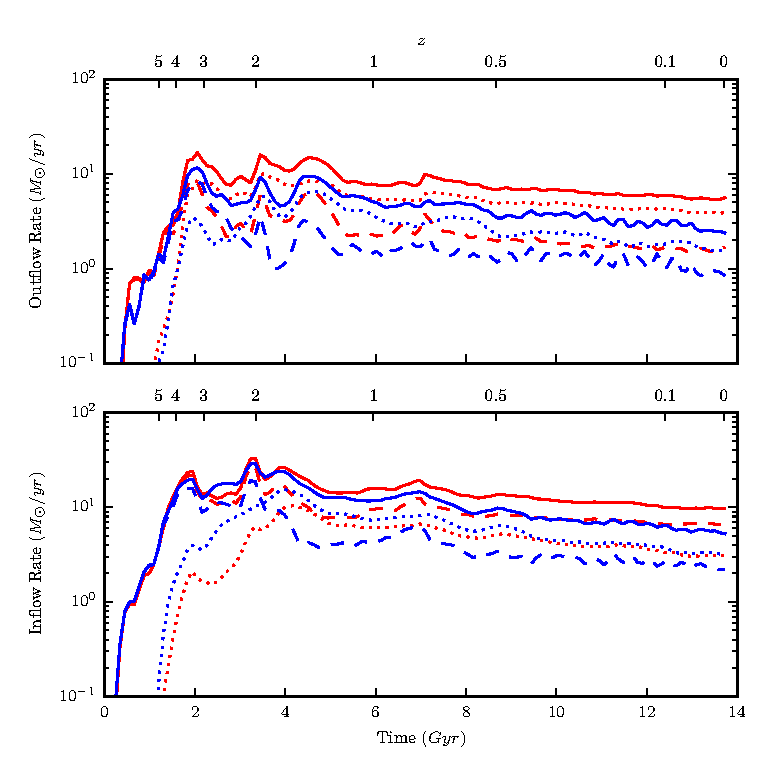
\includegraphics[width=0.8\textwidth]{figures2/inflowoutflow.eps}
    \caption[Inflow and outflow rates for different feedback models]{Inflow and
    outflow rates for superbubble (red) and blastwave (blue) run.  The solid
    lines show the total inflow rate, while the dashed and dotted lines show
    rates for cold and hot gas (above/below $10^5\; \rm{K}$) respectively.  }
    \label{inflow_outflow}
\end{figure}
\begin{figure}
    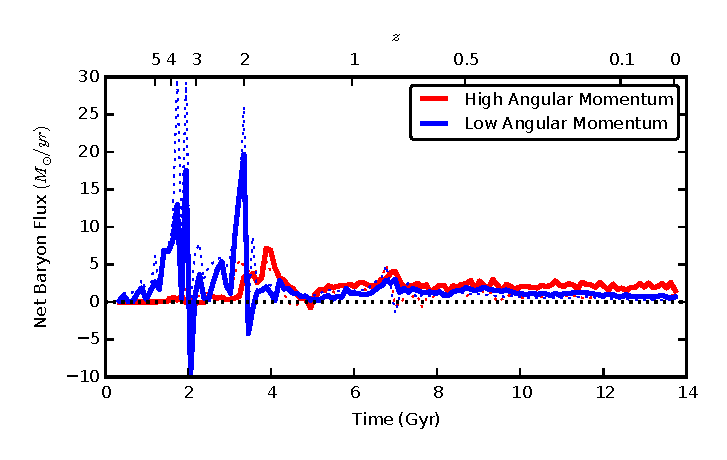
\includegraphics[width=0.8\textwidth]{figures2/angular_momentum_netflux.eps}
    \caption[Net accretion as a function of angular momentum]{In all four test
    cases, including the fiducial superbubble run shown above by the solid
    curve, and the no-feedback case shown by the dotted curve, the vast majority
    of low angular momentum material, with specific angular momentum $ j_z <
    500\; \rm {kpc\; km/s}$, is accreted by $z=2$.  The accretion of high
    angular momentum material, with $j_z > 1500\; \rm{kpc\; km/s}$ rises to peak
    at $z=2$, and continues to accrete $\sim 2\; \rm{M_\odot/yr}$ at $z=0$.  As
    can be seen here, the net flux of low angular momentum material at high
    redshift is suppressed, while the accretion of high angular momentum
    material at low redshift is actually {\it enhanced} by superbubble
    feedback.}
        \label{angular_momentum_netflux}
\end{figure}
Ejecting baryons from the disc is essential to producing galaxies that fit the
$M_*/M_{halo}$ relationship predicted by \citet{Behroozi2013},
\citet{Moster2013} and others.  As Figures~\ref{mass_growth}
and~\ref{stellar_fraction} show, the galaxies either lacking feedback or using
blastwave feedback alone fail to regulate star formation, diverging from the
expected abundance matching relation at $z\sim3$ for the blastwave, and before
$z=5$ without feedback, giving galaxies that lie above the abundance-matching
relationships over nearly their entire history and mass evolution.  With
superbubble feedback, this galaxy lies within the range of observed stellar
masses over its entire evolution, although on the low side of this range at low
redshift.  Arbitrarily increasing feedback energies, despite having reasonable
star formation rates near $z=0$, under produces stars for most cosmic history,
giving stellar masses {\it lower} than predicted by abundance matching.  Stellar
and total masses were calculated for the region inside $R_{vir}$.  As the halo
grows over time, brief reductions in the stellar mass fraction can be seen for
the no-feedback and blastwave feedback halos in Figure~\ref{stellar_fraction},
simply by the accretion of gas and dark matter that has not yet made it to the
galaxy disc.  Once these mergers complete, the stellar fraction rate leaps up
once again because of the new supply of gas.  The relative flatness in this
figure at low redshift is reflected in the relative flatness in the star
formation rate, shown in figure~\ref{sfr}.  This is simply a side effect of the
massive star formation rates at high redshift:  the bulk of star forming gas has
been consumed, and thus star formation has slowed.

The star formation rate, in bins of $150\: \rm{Myr}$, is shown in
Figure~\ref{sfr}.  With no feedback, or blastwave feedback, star formation is
extremely vigorous before $z=2$, slowing at low redshift as gas available for
star formation is exhausted.  With superbubble feedback, star formation is
relatively constant over nearly the entire history of the halo, with only a
gradual increase towards $z=0$.  This apparent quiescence is a function of the
large time window over which we are averaging our star formation rate.  In
Figure~\ref{burstiness}, you can see clearly that despite having an average star
formation rate of $\sim1\; \rm{M_\odot yr^{-1}}$, this is punctuated by bursts
of star formation of as much as $\sim10\; \rm{M_\odot yr^{-1}}$.  Very similar
results were seen in \citet{Muratov2015}, where bursts of star formation are
followed by peaks in the outflow rates.  This burstiness is a important if
stellar feedback is to drive galactic winds:  to generate large superbubbles,
star formation must be clustered in both space and time.  Whether these bursts
of star formation are able to effectively remove baryons from the disc
ultimately depends on the mass loading of the winds that they drive.

\subsection{Outflow Analysis}
\begin{figure}
    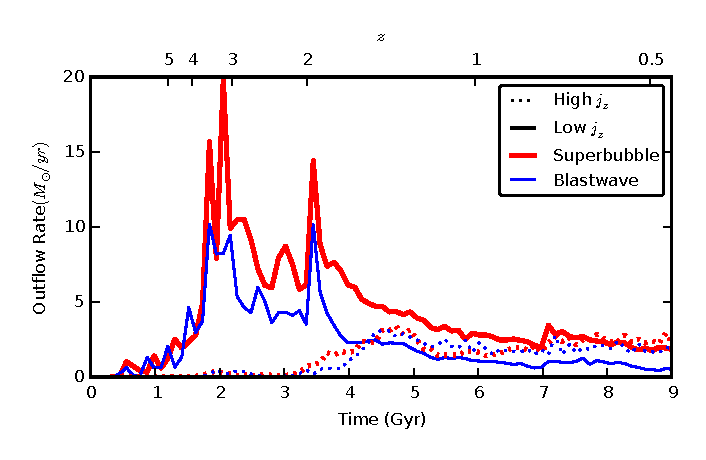
\includegraphics[width=0.8\textwidth]{figures2/angular_momentum_outflow.eps}
    \caption[High redshift winds remove low angular momentum gas]{High-redshift
    winds preferentially remove low angular momentum material.  As can be seen
    here, significantly more low angular momentum material is removed by
    superbubble feedback than by the weaker blastwave feedback, but the amount
    of ejected high-angular momentum material is roughly equal.}
        \label{angular_momentum_outflow}
\end{figure}
\begin{figure}
    \includegraphics[width=0.8\textwidth]{figures2/phase.eps}
    \caption[Gas phase diagram for g1536]{Phase diagram of gas in the halo at $z=0$.  The hot, coronal gas
        with temperatures above $10^5\;K$ contains roughly 40\% of the gas mass
        in the halo.  This gas is a mixture of virial-shocked pristine gas,
        which has never been within the interior $0.1R_{vir}$, and outflowing
        material ejected from the galaxy.  This buoyant, high-entropy gas exits
        the galaxy at high temperature, and cools adiabatically as it rises
        through the CGM.  The three colored contours show the major components
        of this hot coronal gas.  Pristine gas, never falling within the
        interior, is shown in blue.  Young superbubbles, not yet having broken out
        of the galaxy, are shown in red.  Outflowing material that was once inside the
        galaxy but is now cooling adiabatically as it rises through the CGM can be seen
        in orange.  The contours show the 1.5\%, 1\%, and 0.5\% levels for the
        total mass in each cut.}
        \label{phase}
\end{figure}
Star formation in the disc drives hot, fast-moving outflows from the central star
forming regions.  These outflows have temperatures of $\sim2\times10^7\; \rm{K}$
as they leave the disc, and also entrain some cold material with them.
Typically outflow velocities are a few hundred $\rm{km/s}$, less than the
escape velocity of the halo, but sufficient to propel gas to large radii before
it begins to fall in again.  

We calculated inflow and outflow rates and velocities by examining particles
within a spherical shell, with inner radius $0.1R_{vir}$ and outer radius
$R_{vir}$ (giving a shell of thickness $0.9R_{vir}$).  We use the $\bar\rho =
200\rho_{crit}$ definition for $R_{vir}$.  Particles with $v_r < 0$ are
inflowing, while those with $v_r > 0$ are outflowing.
Within this shell, the mass flux is determined simply as:
\begin{equation}
    \dot M = \sum_{r_i\in\mathrm{shell}}\frac{M_i v_i}{0.9R_{vir}}
    \label{halo_massflux}
\end{equation}

As figure~\ref{massloading} shows, the outflow behavior of this galaxy is
fundamentally different when superbubble feedback is used.  The wind mass
loading factor $\eta = \dot M_{outflow} / \dot M_*$, a measure of how
efficiently feedback is generating outflows, is roughly an order of magnitude
larger during the bursts of star formation from $z=4-2$, expelling a large
amount of gas from the disc early on.  The resulting suppression of
high-redshift star formation is key to obtaining the correct stellar mass
relation as the halo grows, is unmistakable in figure~\ref{mass_growth}
and~\ref{stellar_fraction}.  Evidence of these outflows can be seen in the $z=0$
column density images in figure~\ref{column_density}.  High-latitude neutral
hydrogen from both ejected and infalling material can be seen in the two
superbubble cases, but is totally absent otherwise.  The smaller amount seen
around the high feedback energy case is simply due to this gas being expelled
further.  The reason superbubbles are so effective at removing mass from the
galaxy and thus regulating the stellar mass depends both on the higher outflow
rates as well as the lower star formation rates needed to drive these outflows,
leading to much larger mass loading factors than the blastwave model can
achieve.  This is clearly shown in figure~\ref{massloading}, as the top panel is
essentially the middle panel divided by the bottom panel.  The outflow rates
driven by superbubbles is at most $\sim2$ times greater than the blastwave model,
but since this is driven by a comparatively tiny amount of star formation, the
massloading, $\eta$, is nearly 10 times greater at high redshift.  The factor of
$\sim2$ higher outflow rate is what we would expect from the roughly $\sim2$
larger baryon depletion from the superbubble vs. blastwave cases.

The effectiveness of the superbubble-driven galactic winds can be clearly seen
in figure~\ref{net_accretion}, where the net accretion of stars and gas is
greatly reduced by the use of superbubble feedback, resulting at $z=1$ in a net
reduction in the total baryonic mass inside $0.5R_{vir}$ of $\sim14\%$ vs.
blastwave feedback, and $\sim30\%$ vs. no feedback whatsoever (along with the 
removal of baryons from the disc discussed earlier. As the outflow
rate drops towards $z=0$, much of this ejected material falls back onto the
disc, and the outflows transition to a fountain mode, actually increasing
the inflow rate seen compared to the blastwave feedback case in
figure~\ref{inflow_outflow}.  This increase in the accretion of gas fuels an
equivalent increase in star formation, as is seen in figures~\ref{sfr}
and~\ref{massloading}.

Figure~\ref{angular_momentum_netflux} shows that the total accreted gas switches
from being dominated by low angular momentum material to being primarily high
angular momentum material at $z\approx2$.  Because $\eta$ is high ($\sim 10$)
during this period, low-angular momentum material is preferentially ejected from
the galaxy without forming a significant number of stars.  These results agree
quite well with the results of \citet{Muratov2015}, which also found $L^*$
progenitors at $z>2$ had wind mass loadings $\eta\sim 10$. The preferential
ejection of low angular momentum gas is clear in
figure~\ref{angular_momentum_outflow}.  The small amount of high angular
momentum material accreted before $z=1$ is ejected at an essentially equal rate
with or without superbubble-driven winds, but low angular momentum material is
propelled into winds at roughly twice the rate when superbubble feedback is
taken into account.

The phase diagram in figure~\ref{phase} shows that, as expected, the galaxy
contains both a hot halo (in which nearly half of the gas mass can be found),
and contains no gas in regions of short cooling time.  This behavior was shown
previously in the isolated galaxy simulations of \citet{Keller2014}.  The hot
halo gas can be divided into three major components. The coolest component is
pristine, virial shocked material that has not ever been accreted (never passed
within $0.1R_{vir}$ of the halo center).  The hottest gas is actually not yet in
the corona, but is the interior of young superbubbles still within the galaxy
disc.  As this material leaves the disc, it cools adiabatically in the lower
pressure environment of the halo, as can be seen in from the $\rho^{2/3}$
adiabatic path it takes through the phase diagram.  Detailed analysis of this
halo gas, especially in comparison to observations like those of
\citet{Steidel2010}, will be explored in a future study of a larger sample of
L* galaxies.

\section{Discussion}

Past work, especially the Aquila comparison \citep{Scannapieco2012}, has shown
that feedback mechanisms which do not remove a large fraction of baryons from
galaxy discs fail to produce realistic spiral galaxies.  Galaxies simulated
without such feedback show more spheroidal stellar
distributions, older stellar populations, and more total stellar mass than is
observed in nature.  Those cases that do manage to expel enough gas to produce
reasonable stellar mass fractions still fail to produce the correct stellar
kinematics, failing to produce the small bulges characteristic of
so many spiral galaxies.  These models also rely on mechanisms other than
stellar feedback (SMBH heating) or on major numerical contrivances (hydrodynamic
decoupling, etc.).  

Superbubbles offer a way out of this bind. As was shown in \citep{Keller2014},
evaporation in superbubbles naturally mass load winds with temperatures of
$\sim10^7\;K$, a process that is set by self-regulating thermal conduction.
This means that an optimal amount of material is heated above the virial
temperature ($1.3\times10^6\;K$ for a $8\times10^{11}\;M_\odot$ halo).  This
feedback-heated and highly buoyant hot gas migrates out of the disc, cooling
adiabatically while it rises, as is clearly seen in figure~\ref{phase}.   In
fact, as figure~\ref{stellar_fraction} shows, there may even be room to {\it
reduce} the feedback energy below the fiducial $10^{51}\;\rm erg/SNe$, while
still producing reasonable stellar mass fractions.  On top of yielding
physically-realistic galaxies, superbubble feedback is in fact slightly
\textit{less} computationally expensive than blastwave feedback for these
simulations, due in part to its elimination of unphysical high density, high
temperature gas.

\subsection{High-Redshift Outflows Determine Galaxy Properties}

A major failure of other feedback models is 
the production of too many stars, too early.  Superbubble feedback prevents this
by efficiently removing gas from the star forming disc at high redshifts.  The
high mass loadings from $z=2-4$ means more mass is being expelled by
significantly fewer stars.  Mass loadings much larger than unity have been
observed in both Lyman Break Galaxies at high redshift \citep{Pettini2002} and
in local dwarf starburts \citep{Martin2002}.  

Even if a galaxy has the correct stellar mass fraction at $z=0$, forming too
much of your stellar mass at high redshift is problematic for a number of
reasons.  First, it is known from abundance matching as well as the observations
of stellar ages that most stars in $\rm{L^*}$ galaxies are formed fairly late
(e.g. \citet{vanDokkum2013} found $\sim90\%$ of stars in Milky Way like galaxies
formed at $z<2.5$).  Secondly, forming these stars early on means they will be
formed primarily in smaller halos that are subsequently accreted, as well as in
main halo at small radii (as low angular momentum material is accreted first, as
seen in figure~\ref{angular_momentum_netflux}). This results in a stellar
distribution too spheroidal and centrally concentrated, as was seen in many
older simulations, and here in the rotation curves in
figure~\ref{rotation_curve} for the blastwave and no feedback test cases.

Because superbubbles drive strong outflows at high redshift, the galaxy is able
to preferentially remove low angular momentum gas, as indicated by
figure~\ref{angular_momentum_outflow}. This same mechanism  was seen in
simulations of dwarf galaxies by \citet{Brook2011,Brook2012}.  We would suggest
that this is a universal requirement for producing galaxies with low central
concentrations and small bulges.  As \citet{Binney2001} argued, if this gas were
to remain within the disc, it would be ultimately form the massive bulge that is
seen in our blastwave and no feedback cases, and in numerous other past
simulations.  If only a third of the baryons removed in the disc of our fiducial
case were to instead form bulge stars, it would raise the B/T ratio of the disc
to 0.3, making our disc much more bulge dominated than the Milky Way, and
putting our results in conflict with \citet{Allen2006}.  This mechanism (strong,
high-redshift outflows), and the fact that it produces strong suppression of
star formation at high redshift as well as a small stellar bulge, agrees well
with the results of \citet{Sales2012}.  That study of $\sim100$ GIMIC
\citep{Crain2009} galaxies found that those with the smallest B/T ratio also had
the largest fraction of stars formed late in the galaxy's history.  Strong
outflows acting to regulate high redshift star-formation while preserving fuel
for late star formation naturally leads to this situation.

The effectiveness of superbubble feedback may help to prevent the growth of a
massive stellar bulge via a second mechanism as well.  \citet{Fall1980} showed
that the dissipational collapse of hot gas within an extended dark halo can
produce galaxies with thin discs.  However, \citet{Cole2000} showed that the
collisionless processes involved in galaxy mergers can cancel out the net
rotation of a galaxy disc and lead to a spheroidal stellar distribution.  With
superbubble feedback, small dwarves convert very little of their baryonic mass
into stars, allowing them to contribute their gas to the primary halo, which
then collapses dissipationally.  

The heavily mass loaded winds driven by superbubble feedback are not only key to
suppressing high-z star formation, but also to providing enough gas at low
redshift to continue star formation.  The outflows produced by superbubble
feedback can easily escape from the lower-mass progenitors of ${L^*}$ galaxies.
Thus it is able to naturally transition from the violent, wind-driving high
redshift mode to a more quiescent phase as the galactic gravitational potential
and gas surface densities in the disc increase (see the increase in inflow in
figure~\ref{inflow_outflow}.  These factors suppress outflows, and allow star
formation to increase slowly towards $z=0$.

As the disc is assembled, the disc surface density above the 
superbubble increases.  Thus the hot gas must push past
more material and will also entrain more material along with it as shown by
 the clumps seen in figure~\ref{column_density}).  
This slows the outflows compared to those 
seen at high redshift and moving the galaxy
towards a fountain mode.  The gas is kicked to relatively low altitudes and
then rains back down onto the galactic disc.  This effect is probably
sensitive to resolution.  Our small-scale experiments show
 that venting of superbubbles is enhanced by a more porous ISM 
(see \citealt{Keller2014} and also \citealt{Nath2013}).  
Poor resolution suppresses this porosity and increases
numerical dissipation.  Thus better resolution might reduce the puffy
appearance in the HI column density and allow strong galactic
outflows towards $z=0$.  

\subsection{Additional Feedback Mechanisms}

We have shown that, even at moderate resolution, thermal supernova feedback is
sufficient to build a realistic L* galaxy, provided a complete
physical feedback model like that of \citet{Keller2014} is used.    
Thus this work firmly establishes what supernovae and superbubbles can do.

It is still likely that for higher-mass halos $(>10^{12}\; \rm{M_\odot}$),
supernovae alone will not be suffficent to regulate star formation and produce
the drop in star formation efficiency seen in \citet{Moster2013,Behroozi2013}.
We do not include feedback from SMBH, which is likely to be
important for higher-mass galaxies.  

Our resolution limits the formation of dense structures in the ISM.  The lack of
resolved dense gas means that feedback processes involved in disrupting
molecular clouds (UV photodissociation, radiation pressure, etc.) is largely
irrelevant for these simulations.  In fact, since much of the energy from early
stellar feedback is consumed in the disruption of the densest clouds in
simulations such as this, the addition of this energy may be unrealistic,
effectively double counting energy that would have been used to disrupt clouds.
Furthermore, high-resolution studies of individual molecular clouds have found
that ionizing radiation, despite disrupting these clouds, ultimately only
imparts $\lesssim 0.1\%$ of the total radiative luminosity to the gas in the
cloud and the surrounding medium in the form of additional thermal and kinetic
energy \citep{Dale2005, Gendelev2012, Walch2012}).  Thus, applying even as
little as $1\%$ of the radiative luminosity as a source of feedback in a
simulation that does not resolve structure within molecular clouds is likely
massively overestimating the impact on disc scales.

In sufficiently high-resolution simulations it may be necessary to include small
scale feedback mechanisms in order to disrupt clouds before the first SN,
allowing the to explode in a lower density environment since, as
\citet{MacLow1988} showed, the cooling time for superbubbles scales sub-linearly
with the inverse density, $t_R\propto n_0^{-8/11}$.  \citet{Rogers2013} showed
that the disruption of high-density clouds by stellar winds prior to the first
supernovae can allow as much as $99\%$ of the hot SN ejecta to escape into the
surrounding warm ISM, helping to promote the growth of superbubbles that then
vent from the galactic disc.  In the current work, the densities near the
superbubbles are modest and this preprocessing is not required.

\section{Conclusion}

We have shown that supernova feedback alone, with a complete physical
superbubble model, is capable of producing an $\rm{L^*}$ galaxy that falls
within observational constraints.  Superbubbles are a physical mechanism for
producing ab initio galactic winds, that ultimately allow for the formation of a
galaxy with a realistic star formation history and a negligible stellar bulge.

The key results with respect to galaxy formation are as follows:

\begin{itemize}
    \item Strong outflows at high redshift are essential to regulating
        star formation over the total halo history.  The vast majority of stars
        in $\rm{L^*}$ galaxies form after $z\sim2$.  Unless gas is removed from
        galaxies at high redshift by feedback processes, it will rapidly form
        stars, yielding discs that are too massive and red at $z=0$.
    \item Outflows are important for producing the correct disc kinematics and
        preventing the formation of excessive bulges.  Low angular momentum gas
        is accreted first as galaxies form, and the pooling of this gas at the
        center of galaxies can lead to galaxies with sharply peaked rotation
        curves and unrealistically large bulges, often containing the majority
        of stars within the galaxy.  
    \item Galaxies simulated without feedback, or with disabled cooling feedback
        models fail to expel enough of this gas early on, and result in
        bulge-dominated galaxies with unrealistic stellar mass fractions.  The
        superbubble model, on the other hand, produces strong outflows that
        ultimately yield realistic galaxies.
    \item Superbubble feedback naturally yields the sort of outflows that are
        required for $L^*$ galaxies.  The mass-loading \& velocity of
        the winds are set by the hydrodynamics and evaporative mixing, unlike
        other methods where these values are free parameters.
    \item Superbubble feedback produces high-redshift outflows that
        preferentially remove low angular momentum gas, and in so doing,
        prevents the formation of massive bulges and the associated strongly
        peaked rotation curves. It does this without also expelling additional
        high-angular momentum gas, allowing the stellar disc to form while
        arresting the formation of a bulge.
    \item These advantages come without any significant additional computational
        expense, and may in fact be less costly than alternative feedback
        models.
\end{itemize}

Superbubbles are effective up to at least $\rm{L^*}$.   Beyond $\rm{L^*}$, we
anticipate important roles for SMBH feedback or potentially radiation pressure
(see e.g.  \citealt{Hopkins2013}).  In the subsequent MUGS2 series of papers, we
will show how these effects extend to larger and smaller halos forming in a
range of environments.

\section*{Acknowledgements}
The analysis was performed using the pynbody package
(\texttt{http://pynbody.github.io/}, \citep{pynbody}), which was written
by Andrew Pontzen in addition to the authors.  We thank Fabio Governato, Tom
Quinn, Sijing Shen, Greg Stinson, \& Rob Thacker for useful conversations
regarding this paper.  The simulations were performed on the clusters hosted on
\textsc{scinet}, part of ComputeCanada.  We greatly appreciate the contributions
of these computing allocations.  We also thank NSERC for funding supporting this
research.
\bibliographystyle{mnras}
\bibliography{library}

\chapter{Cosmological Galaxy Evolution with Superbubble Feedback II: The Limits
of Supernovae}
\thispagestyle{fancy}
\textit{Reprinted from B.W. Keller, J. Wadsley, \& H.M.P.
Couchman 2016,} \\ \textsc{Montly Notices of the Royal Astronomical Society}
\textit{Volume 463, Issue 2, pp. 1431-1445, DOI: 10.1093/mnras/stw2029
Published by Oxford University Press on behalf of the Royal Astronomical
Society.  All rights reserved}
%\setcounter{pageFix}{\value{page}}
\begin{abstract}
\thispagestyle{fancy}
    \setcounter{page}{\value{pageFix}}
        \addcontentsline{toc}{section}{Abstract}

    We explore when supernovae can (and cannot) regulate the star formation and
    bulge growth in galaxies based on a sample of 18 simulated galaxies.  The
    simulations are the first to model feedback superbubbles including
    evaporation and conduction.  These processes determine the mass loadings and
    wind speeds of galactic outflows.  We show that for galaxies with virial
    masses $>10^{12}\;\Msun$, supernovae alone cannot prevent excessive star
    formation.  This occurs due to a shutdown of galactic winds, with wind mass
    loadings falling from $\eta\sim10$ to $\eta<1$.  In more massive systems,
    the ejection of baryons to the circumgalactic medium falters earlier on and
    the galaxies diverge significantly from observed galaxy scaling relations
    and morphologies.  The decreasing efficiency is due to a deepening
    potential well preventing gas escape, and is unavoidable if mass-loaded
    outflows regulate star formation on galactic scales.  This implies that
    non-supernova feedback mechanisms must become dominant for galaxies with
    stellar masses greater than $\sim4\times10^{10}\;\Msun$.  The runaway growth
    of the central stellar bulge, strongly linked to black hole growth, suggests
    that feedback from active galactic nuclei is the likely mechanism.  Below
    this mass, supernovae alone are able to produce a realistic stellar mass
    fraction, star formation history and disc morphology.
\end{abstract}

\section{Introduction}
Stellar feedback plays many roles in galaxies.  Simply regulating the star
formation rate (SFR) within the interstellar medium (ISM) is not enough to produce a
realistic galaxy population.  The reduced baryon fractions seen in galaxies requires the
expulsion of that gas \citep{Mathews1971,Larson1974}.  Matching observed
scaling relations, cosmic star
formation histories, the stellar mass--metallicity regulation, and the stellar mass
function all require the ejection of gas from a galaxy in large-scale outflows
\citep{Dekel1986,Erb2008,Finlator2008,Peeples2011,Marasco2012}.  Both abundance
matching \citep{Behroozi2013,Moster2013} and gravitational lensing studies
\citep{Hudson2015} find that no galaxies convert more than $\sim25\%$ of their
initial baryonic mass into stars.  The most straight forward explanation for this is the
ejection of a significant fraction of the baryons from the galaxy disc.  

The observational evidence of galactic outflows is impossible to ignore (a
review of both the theory and observations of galactic winds can be found in
\citealt{Veilleux2005}).  From intergalactic metals seen in quasar absorption
lines \citep{Songaila1996,Dave1998,Weiner2009}, to the detection of neutral
\citep{Kunth1998,Morganti2003}, ionized \citep{Heckman1987,Martin2012}, and
molecular \citep{Stark1984} outflowing gas with outflow velocities $\gg
100\;\kms$ \citep{Leroy2015}, we can see that galaxies do not merely
accrete gas: they eject it as well (a detailed study of gas inflows and outflows
can be found in \citet{Woods2014}). In our own Milky Way, X-ray observations
have detected $\sim6\times10^{10}\Msun$ in the $\sim10^6\K$ circumgalactic medium
(CGM) \citep{Gupta2012}, comparable in mass to total baryonic mass of the galactic disc.

In \citet{Keller2015}, we showed that a correct treatment of superbubbles driven
by supernovae (SNe) directly generates strong galactic winds without requiring extra
wind models.  This was the first time the complete physics of thermal conduction
and evaporation required to model superbubbles (see \citealt{Keller2014}) was
employed in galaxy formation simulations.  This removes the need for cooling
shutoffs, hydrodynamic decoupling, or other purely numerical boosts to the
feedback effectiveness and the associated free parameters.  These first
principles outflows give a stellar mass evolution that matches the abundance
matching results \citep{Behroozi2013}.  By removing preferentially low-angular
momentum gas, these outflows can prevent the growth of a large bulge, producing
bulgeless discs like those that are seen in the nearby Universe.

Prior work \citep{Stinson2013,Hopkins2014,Agertz2015} has examined the role of
outflows in enabling galaxies to regulate their baryon content and match
observed relations as a function of their mass.  A common outcome is that
stellar feedbacks are insufficient for higher mass galaxies.  Typically, these
works relied on multiple feedbacks and detailed subgrid models with associated
free parameters.  These additional feedbacks are discussed in more detail in section 2.  They
did not however, include necessary physics to accurately model superbubbles.
Thus the question, what SNe driven outflows can do, has yet to be fully
answered.   For example, \citet{Hopkins2014} has argued that SNe alone
cannot regulate the stellar content of intermediate mass galaxies, let alone the
more massive ones.  

The primary goal of this work is to examine galaxies and their outflows via a suite of
simulated field $L*$ galaxies, the McMaster Unbiased Galaxy Simulations 2
(MUGS2).  We begin with an overview of stellar feedback and galactic outflows
in section 2.  We examine which forms of feedback are most likely to
contribute outflows and also discuss alternatives to SNe.  In section
3,  we describe the MUGS2 sample and simulation methods.  We then examine the
evolution and final state of the galaxy sample in section 4.   As in other work,
we find that galaxies more massive than $10^{12}\;\Msun$ deviate from observed
relations.  In our case, this is where SN-driven winds begin to fail.  We
find a universal relation between the halo/disc mass and outflow mass loadings.
Finally, in section 5, we discuss how stellar mass regulation through SNe
fails, how this manifests in the galaxy properties and how this provides strong
clues that active galactic nuclei (AGN), powered by accretion on to
supermassive black holes (SMBH), must take over the regulation.

\section{What Launches Galactic Outflows?}
The question of what ultimately powers galactic winds has been debated for over
half a century, since the first outflows were discovered in M82
\citep{Lynds1963}.  Unfortunately, neither AGN nor
stellar processes have unambiguous observational signatures in the outflows they
produce \citep{Veilleux2005}.  To complicate matters further, stellar feedback
comes in multiple forms.  Disentangling these adds to the uncertainty of how
galactic outflows are actually generated.  Massive stars deposit energy and
momentum in the ISM through ionizing radiation, radiation pressure on dust
grains, stellar winds, and ultimately explode as SN.  Each of these
processes, in principle, has sufficient energy to drive a galactic outflow.
Radiation, in particular, has orders of magnitude more energy available than the
others \citep{Leitherer1999}.  Driving effective galactic winds requires strong
coupling to the ISM gas and limited cooling losses so that the terminal velocities
are high relative to the escape velocity.  We examine the feedback processes
individually below.

\subsection{Stellar feedback}
\subsubsection{Ultraviolet radiation and {\sc Hii} regions}
The characteristic temperature of gas photoionized by UV radiation is
$\sim10^{4}\K$ \citep{Krumholz2009}, far lower than the virial temperature of
all but the smallest galaxies.  For galaxies with halo masses below $10^9\Msun$,
photoheating and photoionization by UV radiation strongly limits star formation
\citep{Efstathiou1992}.  The characteristic sound speed for gas in {\sc Hii}
regions is $\sim10\;\rm{km/s}$, similar to characteristic turbulent velocities
and escape speeds in molecular clouds.  Even large {\sc Hii} regions, such as 30
Doradus, have been observed to have expansion rates of only $25\;\rm{km/s}$
\citep{Chu1994}, significantly less than what is needed to drive even a weak
galactic fountain.  Thus it is doubtful that UV radiation plays much role in
launching galactic-scale outflows.  

Simulations by \citet{Dale2012} have shown that {\sc Hii} regions alone are
unable to effectively remove gas from their birth clouds, let alone their
galaxies but can alter their structure.  Thus UV can play a local role in
simulations that resolve molecular clouds.

\subsubsection{Radiation pressure}
Radiation pressure on the dust grains in galaxies is a potential driver for
galactic outflows.  \citet{Murray2011} showed that, assuming spherical symmetry,
the most massive star clusters can drive reasonably fast ($v\sim$ hundreds of
km/s) outflows.  \citet{Agertz2015} and \citet{Hopkins2014} also found that a
combination of SN, stellar winds, and radiation pressure produced a galaxy which
matched the abundance-matched stellar mass fractions of \citet{Behroozi2013}.
However, as \citet{Agertz2015} noted, and \citet{Roskar2014} examined in detail,
these simulated galaxies often displayed unrealistic morphologies, with much
thicker discs than would be expected for a normal Milky Way like disc.
\citet{Roskar2014} found the addition of radiation pressure using a local `UV
escape probability' model for dust absorption, with a single parameter for the
IR dust opacity $\kappa_{\rm IR}$ was able to reduce the stellar mass fraction of a
cosmological galaxy with mass comparable to the lighter members of our
well-regulated population.  However, this required large values of
$\kappa_{\rm IR}$, such that the UV radiation coupled to the ISM so strongly that
the entire disc was completely disrupted, and the resulting galaxy was
completely spheroidal, with stellar scale heights above $3\;\kpc$.

The porosity of the ISM can significantly reduce the mean optical depth of the
galaxy, giving photons an escape valve to leave unimpeded \citep{Krumholz2013}.
The importance of radiation pressure remains an open question.

\subsubsection{SNe and stellar winds}
Based on energetics alone, it might seem that SN alone could eject gas from even
the most massive haloes.  A Type II SN releases $\sim10^{51}\;\rm{erg}$ in an
ejecta of $\sim10\;\Msun$ \citep{Leitherer1999}. This results in a maximum
ejecta temperature of $\sim2\times10^8\K$.  This corresponds to the virial
temperature for haloes with a mass of $\sim10^{15}\;\Msun$.  This fails to take
into account the mixing of SN ejecta with the surrounding ISM.   Additionally,
if SN ejecta left a galaxy without any mixing or entrainment of additional gas,
the largest wind mass loadings seen would be $\eta\sim0.1$.  Such winds would
remove metals from the ISM but have little effect on the total baryon content.
In order to moderate both star formation and bulge growth, mass loadings of
$>10$ are necessary.  Mixing in cooler ISM material reduces the effective wind
temperature to $\sim10^6\K$ if cooling losses are small.

While it is well known that individual SNe experience strong cooling,
clustered star formation allows SNe and stellar winds to combine into a
superbubble that retains 65 \% of its initial injected energy even after the
formation of cold shell which then breaks out of the ISM into the halo
\citep{MacLow1988}.  With low density channels up to 99 \% of the energy can
escape \citep{Rogers2013}.  An important function of the early stellar feedbacks
discussed earlier is to clear dense gas around the star cluster to enable the
superbubble to escape.  However, as discussed previously, this is only valid in
a simulation if dense gas is resolved.  Thus superbubble feedback can be much
more efficient than SN feedback.  The physics of evaporation also leads
to specific predictions with respect to mass loading and outflow temperatures
of order $\sim 10^6\K$ \citep{Keller2014}.

The virial temperature of haloes with masses of a few $10^{12}\;\Msun$ is
$\sim10^6\K$.  If the wind fluid is cooler than the virial temperature, it will
not rise buoyantly out of the disc into the CGM.  This suggests SN driven winds
become less effective, and may fail to launch altogether somewhere in the mass
range of $\sim10^{12}\;\Msun$. The existence of a peak in the star formation
efficiency at this same mass, as seen in \citet{Behroozi2013} is strong evidence
that this indeed occurring in nature, and that some other feedback mechanism
begins to dominate at higher masses.  Finding out the if, when and how of this
transition is important if we want to know how larger galaxies quench their star
formation, and if SN alone can explain the low star formation efficiency in
galaxies below this mass.

\subsection{Other Feedback Mechanisms}
\subsubsection{AGN}
The primary non-stellar energy source available for driving galactic outflows is
AGN feedback from the growth of SMBHs.  The Milky Way's
own SMBH has a mass of $M_{\bullet}\sim4\times10^{6}\;\Msun$ \citep{Meyer2012}.
The energy released by its formation is
$M_{\bullet}c^2\sim7\times10^{60}\;\rm{erg}$.  This is significantly greater
than the binding energy of the galactic halo ($\sim10^{59}\;\rm{erg}$).  If even
a small fraction of this energy couples to the ISM as it is released, it can
have a significant disruptive effect.  SMBHs are ubiquitous and larger ones are
strongly linked to the presence of massive bulges
\citep{Magorrian1998}.

Much effort has gone into developing sub-grid models for AGN feedback and SMBH
growth, and now AGN feedback is a major component of many large box simulations
(e.g., Illustris \citet{Sijacki2015}; EAGLE \citet{Crain2015}; Rhapsody-G
\citet{Hahn2015}; Horizon-AGN \citet{Dubois2014}).

\subsubsection{Cosmic rays}
Cosmic rays (CRs) have been proposed as another potential engine for
driving outflows \citep{Ipavich1975,Breitschwerdt1991,Everett2008,Socrates2008}.
CRs could be directly linked to SN shocks or shocks within the ISM.
CRs may contain as much energy as the thermal and magnetic components of
a galaxy \citep{Zweibel1995}.

\citet{Jubelgas2008} found CR had little impact on higher mass galaxies.
\citet{Girichidis2015} showed that CRs can launch winds with mass
loadings of order unity for gas surface densities comparable to the Milky Way.
\citet{Salem2014} and \cite{Booth2013} found CR driven outflows had even lower
mass loadings for Milky Way mass haloes.  These results make it doubtful that
CRs are centrally important for galactic outflows.


\section{Methods: MUGS2}
The simulations presented here are the new MUGS2 simulations.  The original MUGS
sample, presented in \citet{Stinson2010},  followed the evolution of isolated,
Milky Way like disc galaxies using low temperature metal cooling, UV background
radiation, and stellar feedback. The new MUGS2 sample includes all of this, 
plus a number of improvements to the hydrodynamic method, along with
the new superbubble feedback model \citep{Keller2014}.  This has resulted in
significantly different evolution in the MUGS2 sample compared to the original
MUGS set, most notably greatly reduced star formation in nearly every galaxy
(the original MUGS sample greatly overproduced stars).

These simulations were run using the modern smoothed particle hydrodynamics
(SPH) code {\sc gasoline2}, as in \citet{Keller2015,Keller2014}.
The changes in this new code include a sub-grid model for turbulent mixing of
metals and energy \citep{Shen2010}, and a modified pressure force form similar
to that proposed by \citet{Ritchie2001}, which is functionally equivalent to
\citet{Hopkins2013}.  Details of the star formation and gas physics model can be
found in \citet{Keller2014}.

\subsection{Simulation ICs}
We adopt the same initial conditions (ICs) that were used in the original
\citet{Stinson2010} MUGS sample.  These cosmological zoom-in ICs were selected
from a $50 h^{-1}\;\rm{Mpc}$ cube, run (with dark matter only) to $z=0$.  The
simulations use a {\it WMAP3} $\Lambda\rm{CDM}$ cosmology, with $H_0 =
73\;\rm{km/s/Mpc}$, $\Omega_M = 0.24$, $\Omega_{\rm bary} = 0.04$, $\Omega_\Lambda =
0.76$, and $\sigma_8 =0.76$.  Galaxies that had halo mass from
$5\times10^{11}\Msun$ to $2\times10^{12}\Msun$ were then selected from the
dark matter only run.  Isolated galaxies were then selected by choosing only
ones which had no neighbours in this mass range within $2.7\Mpc$.  As galaxies
with massive neighbours may be affected by their hot haloes, or radio-mode AGN
feedback, we exclude those galaxies to avoid the need to simulate a much larger
volume, and to focus on the effects of stellar feedback processes.  This
resulted in a sample of 276 candidate haloes, of which the final MUGS sample was
simply selected at random from this pool.  While only nine of these were presented
in \citet{Stinson2010}, subsequent papers presented the remaining galaxies
\citep{Bailin2010,Nickerson2011,Nickerson2013}, and what we present here is the
full set of galaxies that were produced for MUGS.

Each of these simulations has a gas mass resolution of
$M_{\rm gas}=2.2\times10^5\Msun $, and uses a gravitational softening length of
$\epsilon=312.5\; \rm{pc}$, and a minimum SPH smoothing length set to 1/4 of
this.  The total sample presented here consists 18 galaxies, with $z=0$ virial
masses in a range from $3.7\times10^{11}\;\Msun$ to $2.1\times10^{12}\;\Msun$.

\subsection{Star Formation}
We use a standard Schmidt-law star formation recipe, where the rate is set by
the freefall time of gas and an efficiency $c_*$: \begin{equation} \dot \rho_* =
\frac{c_*\rho}{t_{\rm ff}} = c_*\sqrt{\frac{32G}{\rm 3\pi}}\rho^{3/2} \end{equation} We
used an efficiency of $c_*=0.05$, as was used for the original MUGS simulations
\citep{Stinson2010} and in \citet{Keller2015}.  Star formation is only allowed
to take place in gas which satisfies three criteria: it has a temperature below
$1.5\times10^4\K$, density above $9.6\;\rm{cm^{-3}}$ (the density where
gravitational softening becomes important), and is in a converging flow
($\nabla\cdot \boldsymbol{v} < 0$).  This density threshold is larger than that used
in \citet{Stinson2010} (which used $0.1\;\rm{cm^{-3}}$), but identical to that
used in \citet{Stinson2013}.  We have used this larger threshold (as
\citealt{Governato2010} recommends) to better capture the effects of clustered
star formation.  Aside from this higher star formation threshold, our star
formation recipe remains unchanged from the original MUGS sample.

\subsection{Superbubble Feedback}
\begin{table*}
\begin{tabular}{rrrrrrrrrr}
	\hline
	Galaxy & $M_{\rm vir}$ & $\lambda'$ & $f_b$ & $z_{1/2}$ & $z_{\rm lmm}$ & $M_*$ & $M_{\rm gas}$ & $M_{\rm central}$ & $SFR_{\rm z=0}$ \\
	ID&&&&&&  (masses & in & $10^{10}\;M_\odot$) & $(M_\odot\; yr^{-1})$ \\
	\hline
	\hline
	g7124 & 36.6 & 0.039 & 0.150 & 0.8 & 2.1 & 0.5 & 5.0 & 1.8 & 0.6 \\
	g5664 & 47.7 & 0.028 & 0.173 & 0.8 & 3.0 & 0.9 & 7.3 & 3.0 & 1.7 \\
	g8893 & 58.0 & 0.065 & 0.170 & 1.0 & 0.8 & 0.7 & 9.1 & 2.6 & 1.0 \\
	g1536 & 64.9 & 0.029 & 0.189 & 1.0 & 4.0 & 1.9 & 10.4 & 5.2 & 3.9 \\
	g21647 & 74.4 & 0.069 & 0.152 & 0.2 & 0.5 & 1.2 & 10.1 & 3.1 & 2.7 \\
	g422 & 76.2 & 0.033 & 0.183 & 0.8 & 0.7 & 1.5 & 12.4 & 5.1 & 3.2 \\
	g22437 & 85.2 & 0.013 & 0.192 & 0.7 & 2.6 & 9.0 & 7.3 & 11.2 & 17.9 \\
	g22795 & 85.2 & 0.009 & 0.178 & 1.1 & 3.8 & 10.6 & 4.6 & 11.7 & 6.2 \\
	g3021 & 97.8 & 0.040 & 0.192 & 0.6 & 1.7 & 3.6 & 15.1 & 9.9 & 15.7 \\
	g28547 & 98.5 & 0.106 & 0.186 & 0.4 & 0.1 & 1.6 & 16.7 & 4.5 & 2.7 \\
	g19195 & 101.6 & 0.039 & 0.162 & 0.7 & 0.7 & 7.1 & 9.3 & 9.7 & 20.3 \\
	g24334 & 102.2 & 0.052 & 0.174 & 0.5 & 1.6 & 2.6 & 15.3 & 7.2 & 6.8 \\
	g4720 & 102.5 & 0.015 & 0.192 & 0.8 & 1.8 & 14.2 & 5.5 & 14.4 & 8.3 \\
	g4145 & 119.5 & 0.033 & 0.193 & 0.9 & 1.4 & 15.0 & 8.1 & 16.9 & 20.9 \\
	g25271 & 125.5 & 0.016 & 0.187 & 1.1 & 4.0 & 15.6 & 7.9 & 17.0 & 9.7 \\
	g15784 & 131.2 & 0.037 & 0.186 & 1.3 & 7.3 & 13.0 & 11.4 & 17.7 & 9.6 \\
	g15807 & 203.2 & 0.026 & 0.191 & 1.0 & 2.5 & 21.4 & 17.5 & 25.4 & 11.9 \\
	g27491 & 214.7 & 0.039 & 0.184 & 0.7 & 1.1 & 18.8 & 20.8 & 26.6 & 17.6 \\
	\hline
\end{tabular}

    \caption[Summary of MUGS2 galaxy properties]{Redshift 0 properties of the
    full MUGS2 sample.  All masses and particle counts are measured within a
    $R_{\rm vir}$ sphere centred on the halo, except for $M_{\rm central}$,
    which is measured within a $0.1\;R_{\rm vir}$ sphere.}
\label{z0_table3}
\end{table*}
\begin{figure*}
    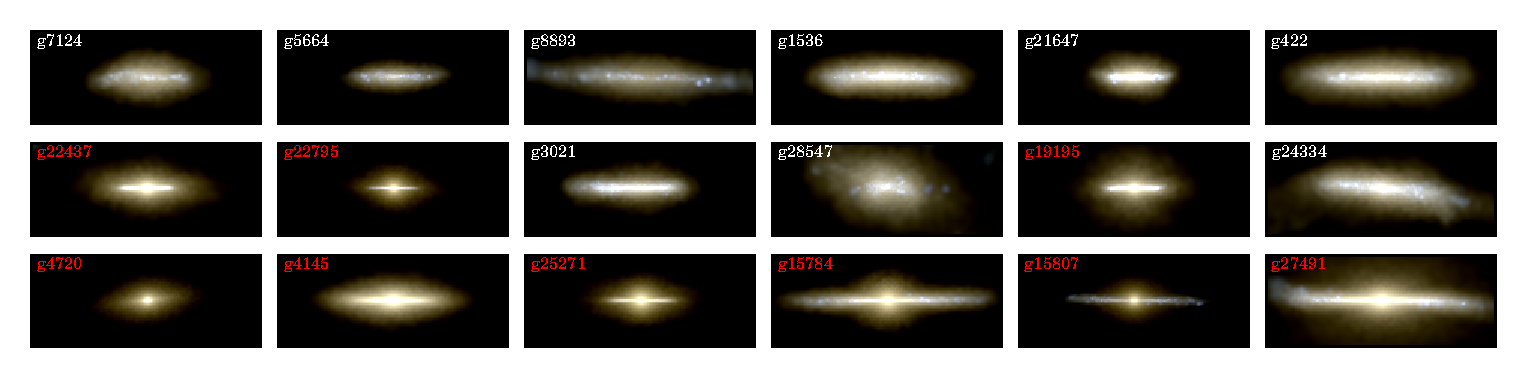
\includegraphics[width=\textwidth]{figures3/stellar_edge.eps}
    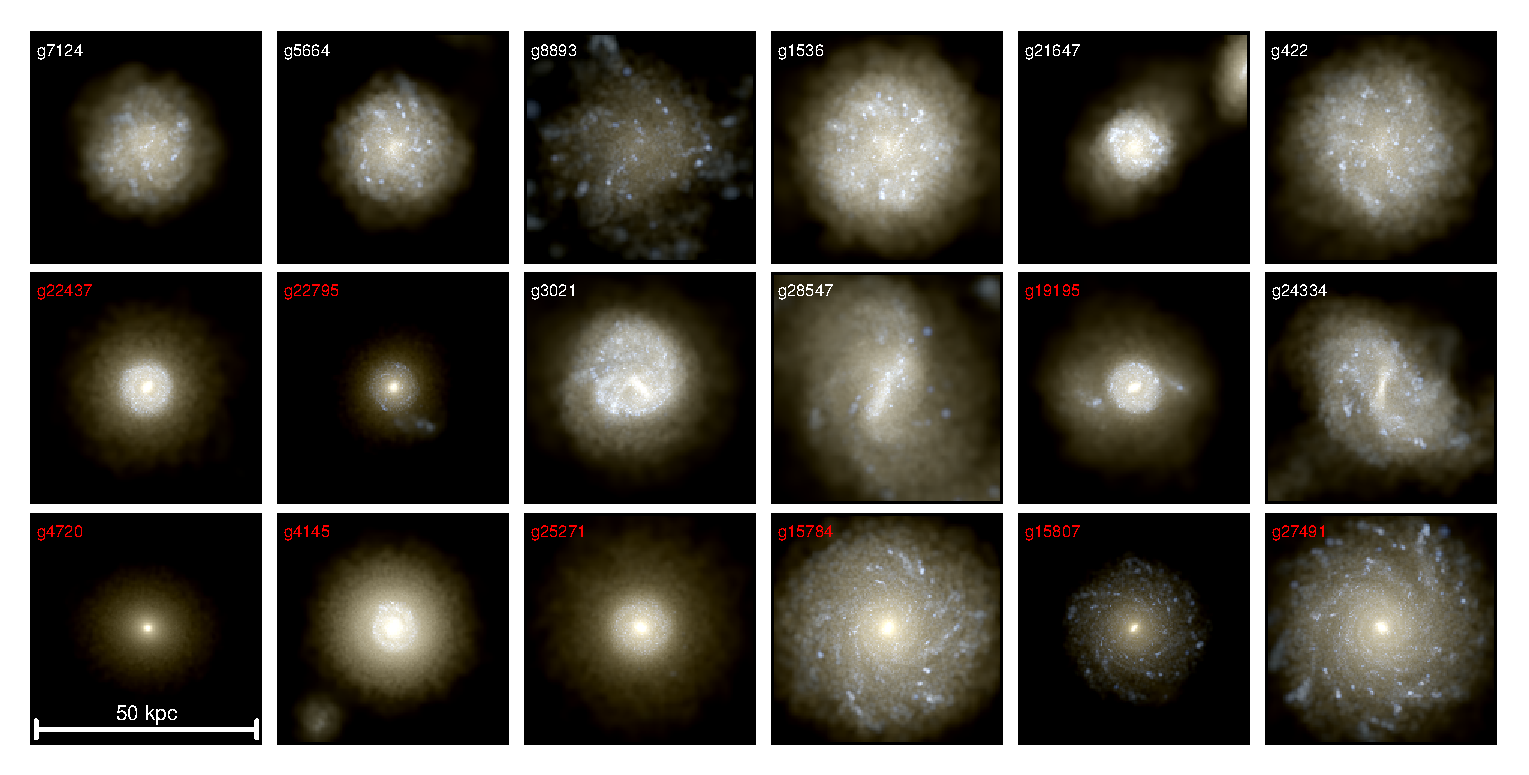
\includegraphics[width=\textwidth]{figures3/stellar_face.eps}
    \caption[Mock stellar images of MUGS2 galaxies]{Mock optical stellar
    observations of each MUGS2 galaxy.  RGB channels are calculated using
    \citet{Marigo2008} stellar populations.  The top three rows show the
    galaxies edge on, while the bottom three show the galaxies face on.  The
    galaxies are sorted in order of halo mass, and galaxies that overproduce
    stars are labelled with red.  These images do not include the effects of
    dust extinction}
    \label{stellar_image3}
\end{figure*}

We use the superbubble feedback model described in \citet{Keller2014}.  We
briefly summarize the important details below.  The model deposits thermal
energy and mass into resolution elements in a brief multi-phase state.  These
particles each have separate specific energies and masses for the hot bubble and
cold ISM components, including the swept up shell.  This allows the method to
calculate a separate density, temperature, and cooling rate for each phase,
rather than using the average density and temperature of both phases.
Multiphase particles are also prevented from forming stars if the average
temperature of the two phases is above our temperature threshold for star
formation.  The amount of SN feedback per unit stellar mass is determined
using a \citet{Chabrier2003} IMF.  

In \citet{Keller2014}, we demonstrated that superbubble feedback could produce
significantly more mass-loaded outflows and reduced star formation in
simulations of isolated disc galaxies, compared to the older \citep{Stinson2006}
blastwave model.  The effectiveness of this older model is highly dependent on
numerical parameter choices.  In \citet{Keller2015} (which examined the first
simulation of the full MUGS2 sample we present here) we chose parameters to
match the original MUGS, and the MAGICC runs of \citet{Stinson2013}. We also
showed how the ISM phase behaviour in superbubble-regulated galaxy behaved in a
much more physically reasonable way than in a galaxy regulated with single
phases.  \citet{Keller2015} showed that in a cosmological galaxy (one of the
same galaxies presented here in the MUGS2 sample, g1536) superbubble feedback
resulted in high mass loadings $\eta\sim10 $ for galactic outflows from
$z\sim\operatorname{4-2}$, which then fell to $\eta\sim1$ at low redshift, producing a galaxy
with a realistic star formation history and no significant bulge component,
without the need for additional feedback mechanisms, or greater feedback
energies than what are provided for simply by SN alone.  We also showed that
this comes without additional computational cost, or the addition of any new
free parameters/tuning.

Aside from a different star formation density and temperature threshold, the
star formation and feedback recipes used here are identical to those used in
\citet{Keller2014}.  One of our sample, g1536, was presented earlier in
\citet{Keller2015}.

\subsection{Comparison to Other Feedback Models}
With $\sim10^{51}\; \rm{erg}$ coupled to the ISM per SN this gives
$1.08\times10^{49}\; \rm{erg}\;\Msun^{-1}$ for the full stellar population.
Comparing this injection rate to other `modern' feedback methods, we typically
are injecting much less energy (and no momentum, which is generated for us
simply through pressure work and the hydrodynamic solver).  For example, the
Illustris simulations \citep{Vogelsberger2014b} use the \citet{Springel2003} ISM
model, with a \citet{Chabrier2003} IMF, giving a total heating rate of
$1.73\times10^{49}\; \rm{erg}\Msun^{-1}$, which along with the
$1.09\times10^{51}\;\rm{erg}$ per SN injected for the kinetic wind model, gives
a total heating rate from SNII of $3.6\times10^{49}\;\rm{erg}\Msun^{-1}$.  The
kinetic winds have their hydrodynamics decoupled from the surrounding ISM,
ensuring no losses from shock-heating and radiative cooling (see
\citealt{Vogelsberger2013,Vogelsberger2014a} for more details on the Illustris
feedback model).  

The EAGLE simulations \citep{Crain2015} use a purely thermal
injection for SNII feedback.  The energy per SN depends on both the local
density and metallicity of the gas that feedback is deposited in, determined
using equation~\ref{eagle3}.
\begin{equation}
    E_{\rm SN} = 0.3 +
    \frac{2.7}{1+\left(\frac{Z}{0.1\Zsun}\right)^{0.87}\left(\frac{n_H}{0.67\rm{cm}^{-3}}\right)^{-0.87}}
    \label{eagle3}
\end{equation}
This gives a total SNII energy of $3\times10^{50}\;\rm{erg}$ in the limit of
infinite metallicity or zero density, and $3\times10^{51}\;\rm{erg}$ in the
limit of zero metallicity or infinite density.  The injection rate is thus
$5.2\times10^{48}\;\rm{erg}\Msun^{-1}$ to
$5.2\times10^{49}\;\rm{erg}\Msun^{-1}$, depending on the local gas properties.
Both the EAGLE and Illustris simulations also include feedback from AGN.  

The FIRE Simulations \citep{Hopkins2014} use a number of mechanisms for stellar
feedback, described in \cite{Hopkins2011}, \citet{Hopkins2012a}, and
\citet{Hopkins2012b}.  This includes radiation pressure, SNe, stellar
winds, photoionization, and photoelectric heating.  The FIRE simulations assume
a slightly less top-heavy \citep{Kroupa2003} IMF.  Radiation pressure is
calculated both as a local deposition of momentum, along with a treatment for
long-range radiation pressure from escaped photons.  The local momentum
deposition is calculated simply using the optical/UV luminosity and an estimated
optical depth for IR scattering: $\boldsymbol{\dot P_{rad}} = (1+\tau_{\rm IR})L/c$.
For this IMF, this gives a total optical/UV energy, integrated over the 1 Gyr,
of $2.25\times10^{51}\;\rm{erg}\Msun^{-1}$.  Naturally, the more mass this is
deposited into the lower the total kinetic energy.  This is, though, the
absolute upper limit of energy available for radiation pressure.  SNe
energy and stellar winds are deposited either as thermal energy, with a total
energy of $2.2\times10^{49}\;\rm{erg}\Msun^{-1}$, or as momentum in the case
when the cooling radius is unresolved.  The photoionization model in FIRE,
described in \citet{Hopkins2012a} uses the ionizing photon rate from
\citet{Leitherer1999} to ionize an equivalent number of neutral hydrogen atoms.  This
gas is heated to, and disallowed to cool below, $T_{HI}=10^4\;K$ in the current
timestep if the ionization rate is greater than the recombination rate.  The
total integrated ionizing photon number is $N_{\rm ion} =
6.6\times10^{61}\;\Msun^{-1}$.  We can estimate the maximum energy injected by
this photoionization model as $E_{\rm ion} = \frac{3}{2}N_{\rm ion}k_BT_{HI} =
1.4\times10^{50}\;\rm{erg}\Msun^{-1}$.  Summed, the total feedback energy
available in the FIRE simulations is $2.41\times10^{51}\;\rm{erg}\Msun^{-1}$.
It should be noted that this is of course an upper limit, and the algorithms
used for FIRE have both local physical and numerical dependencies that can make
the actual values significantly lower than this.  Determining the exact amount
of energy typically deposited is difficult given these complexities.

High-resolution simulations of molecular cloud
disruption by radiation pressure \citep{Dale2005,Gendelev2012,Walch2012} have
found that $\lesssim 0.1\%$ of the radiative luminosity couples to the ISM around
the cloud in the form of momentum or thermal energy.  Instead, as the
simulations of \citet{Rogers2013} showed, the energy release by stellar winds
prior to the first SN instead disrupt the densest gas,
producing channels that allow SN to detonate in a less dense environment, where
cooling times are longer.  Thus, in simulations such as these which do not
resolve dense molecular gas, including the effects of radiation pressure and
stellar winds likely overestimate their effect, as the dense gas 
whose disruption absorbs their energies is not present in the simulation.

\section{Results}


\subsection{Redshift zero properties}
\begin{figure}
    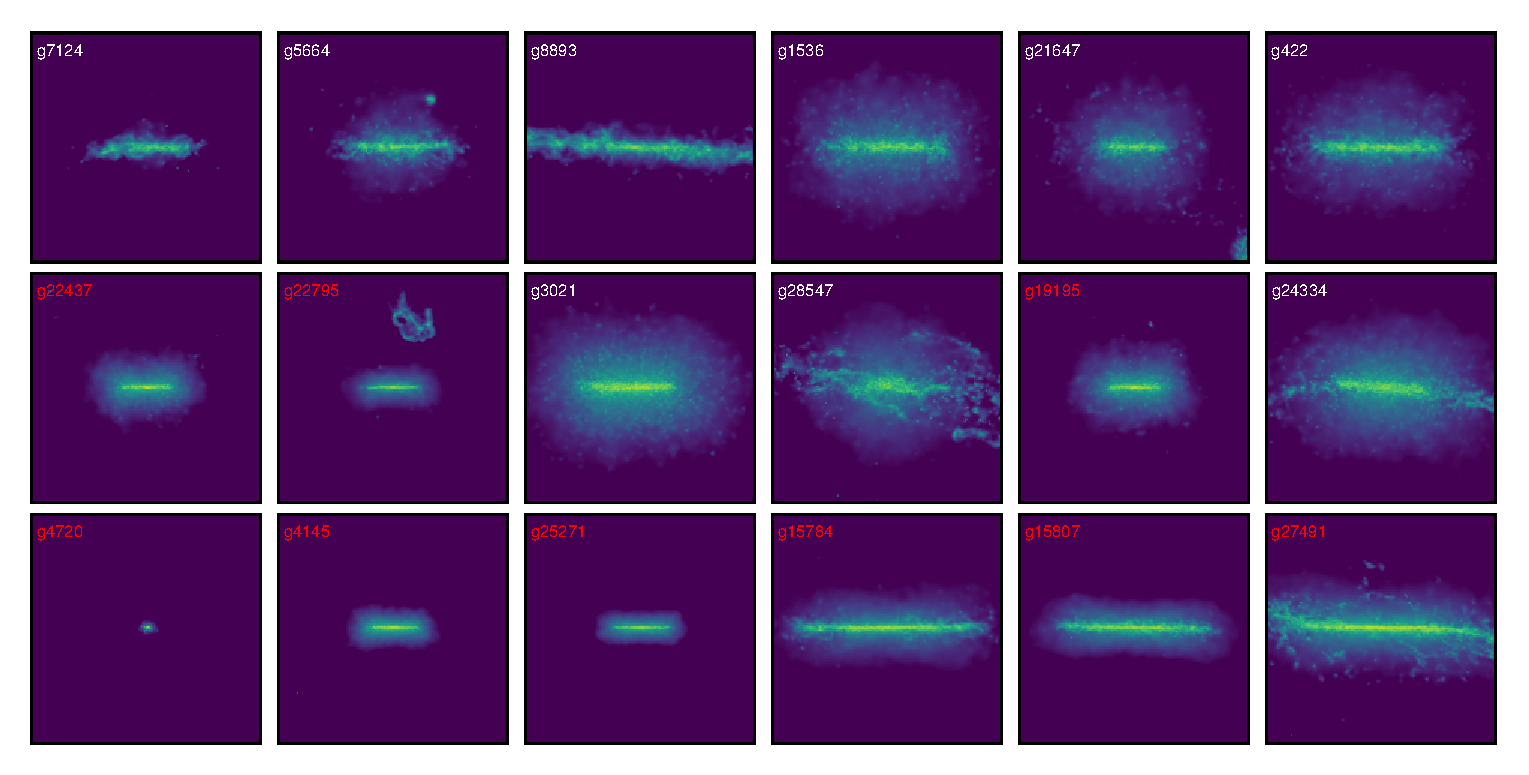
\includegraphics[width=\textwidth]{figures3/column_edge.eps}
    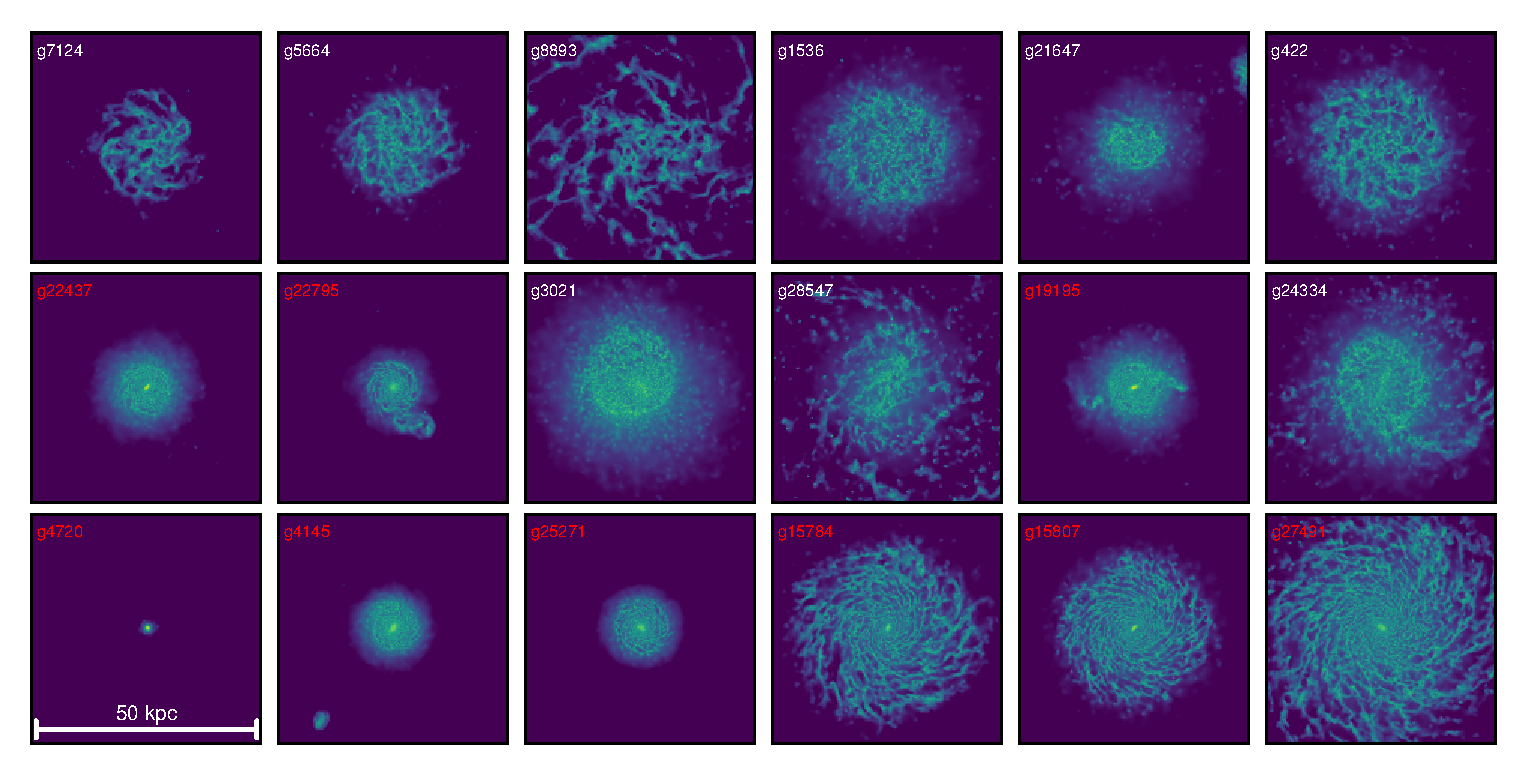
\includegraphics[width=\textwidth]{figures3/column_face.eps}
    \caption[HI column density images for MUGS2 galaxies]{{\sc Hi} column
    density in each of the MUGS2 galaxies.  As in Fig.~\ref{stellar_image3}, the
    top three rows show the galaxy edge on.}
    \label{gas_column3}
\end{figure}
\begin{figure}
    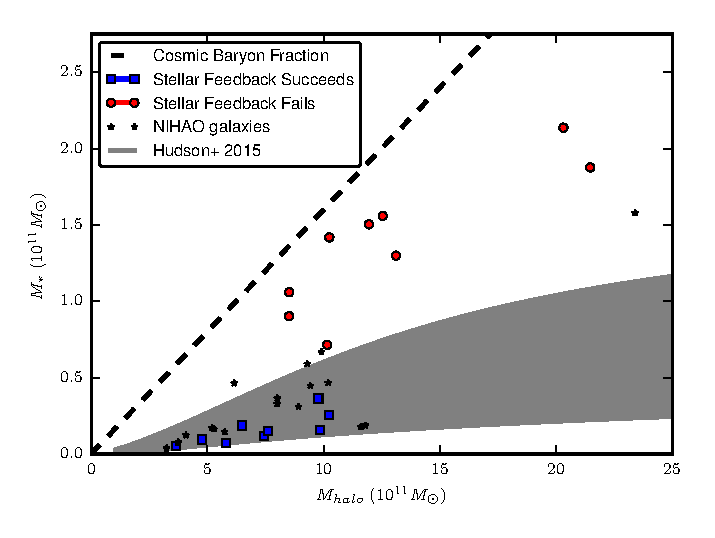
\includegraphics[width=0.7\textwidth]{figures3/SMHMR.eps}
    \caption[MUGS2 stellar mass to halo mass relation]{Stellar mass versus halo
    mass at $z=0$.  The observed stellar mass to halo mass relation is from
    \citet{Hudson2015}'s weak lensing study of galaxies to $z=0.8$.  Galaxies
    that fall within this range are shown as blue squares, while galaxies above
    the curve (those which form too many stars) are shown as red circles.  For
    comparison, the black stars show galaxies from the NIHAO sample
    \citep{Wang2015}.}
    \label{SMHMR3}
\end{figure}
\begin{figure}
    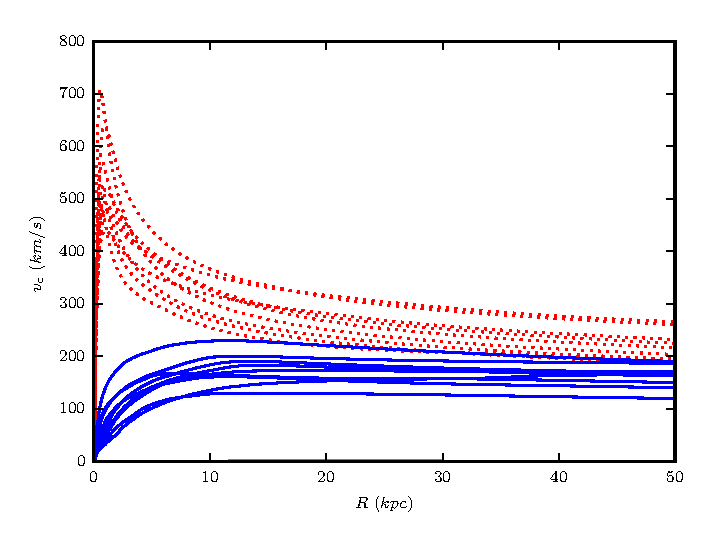
\includegraphics[width=0.7\textwidth]{figures3/rotcurve.eps}
    \caption[MUGS2 rotation curves]{As is clear from the above rotation curves,
    galaxies which overproduce stars (shown in dotted red) also have large
    central concentrations, giving steeply peaked rotation curves inconsistent
    with those seen in local $L*$ galaxies.  Galaxies with well-regulated star
    formation have flat rotation curves (shown in solid blue).}
    \label{rotation_curve3}
\end{figure}
\begin{figure}
    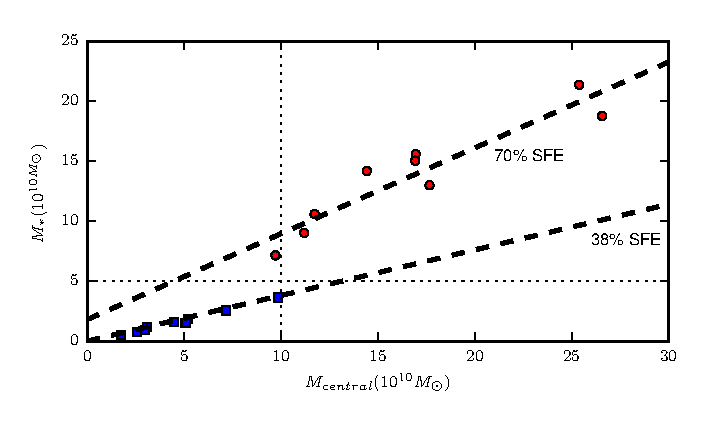
\includegraphics[width=0.8\textwidth]{figures3/stellar_central.eps}
    \caption[Stellar mass vs. central baryonic mass in MUGS2 galaxies]{The stellar mass and the central baryonic mass show a tight
        correlation.  For the well-regulated population, roughly $40\%$ of the
        central baryons are stars, while for the unregulated population has
        converted $\sim70\%$ of the central baryon mass into stars.}
    \label{stellar_central3}
\end{figure}
\begin{figure}
    \includegraphics[width=0.63\textwidth]{figures3/phase.eps}
    \caption[Gas phase diagram in two MUGS2 galaxies]{Gas phase diagrams for a
    well-regulated galaxy (g24334) and an unregulated galaxy (g19195).  Colour
    shows the amount of mass at a given $\rho-T$ point.  The top phase diagram
    shows the characteristic slope for adiabatic (dashed line) and isobaric
    (dotted line) processes.  As can be seen, both galaxies are qualitatively
    the same.  Both show the equilibrium cooling curve below $10^4\K$, and both
    show the adiabatic evolution of superbubble-heated gas as it leaves the
    disc.}
    \label{phase3}
\end{figure}

The general properties of each galaxy at $z=0$ can be found in
Table~\ref{z0_table3}.  $\lambda'$ is the dimensionless spin parameter of the
halo, defined by \citet{Bullock2001} as $\lambda'=J/\sqrt{2GM_{\rm vir}^3R_{\rm vir}}$.
$f_b$ is the baryon fraction of the halo.  $z_{1/2}$ and $z_{\rm lmm}$ are the
redshifts at which the halo reaches half of its final mass, and the redshift of
last major merger respectively.  Major mergers are defined to match
\citet{Stinson2010}, as a merger with a halo containing at least $1/3$ the
stellar mass of the main progenitor.  $M_{\rm vir}$, $M_*$, and $M_{\rm gas}$ are the
masses of the full halo, the stellar component, and the gas component
respectively within the virial radius.  $\rm{SFR_{\rm z=0}}$ is the redshift 0 
SFR, averaged over the previous $100\Myr$.  The virial radius
is defined as the radius around the halo such that the enclosed density is 200
times the critical density ($\rho=200\rho_{\rm crit}$).  While we used the same
definitions for quantities reported in \citet{Stinson2010}, every value reported
here is derived from the new MUGS2 simulations.  We also define a {\it central}
region of the halo, which contains the disc and the majority of the stars within
the halo.  The baryon mass within this region is given as $M_{\rm central}$.  This
central region is simply a sphere of radius $0.1R_{\rm vir}$.

Mock stellar observations and {\sc Hi} column images of these galaxies can be
seen in Figs~\ref{stellar_image3} and~\ref{gas_column3}.  The labels on each of
these images are coloured red if they are in the `unregulated' population
discussed in the next section.  The varied merger history of these galaxies is
evident in these images: companions can be seen in three galaxies (g21647,
g22795, g4145), tidal tails are evident in another  (g19195), and strong bars
exist in another two (g28547, g24334).  

The {\sc Hi} column density shown in Fig.~\ref{gas_column3} shows, as was seen in
\citet{Keller2015}, large quantities of extraplanar {\sc Hi} gas, driven up by
outflows from the galaxy disc.  {\sc Hi} gas above the galactic plane has been seen
since \citet{Muller1963}.  \citet{Lockman1984} found similar column densities to
what is seen here to heights of $1.5\kpc$.  High-velocity clouds of relatively
dense ($\sim0.1\; \rm{cm^{-3}}$) gas have also been seen both leaving and
returning to the galaxy \citep{Wakker1997}.  Diffuse {\sc Hi} gas has been observed
out to $\sim300\kpc$ in absorption features of numerous nearby galaxies
\citep{Wakker2009,Prochaska2011}.  \citet{Werk2014} surveyed a number of
galaxies in the COS-haloes survey, and found that typical $L*$ galaxies contain
$\sim5 \times10^{10}\Msun$ of cool gas in their CGM.  The face-on {\sc Hi}
distribution for all but a handful of the unregulated (see the following
section) follow the \citet{Broeils1997} {\sc Hi} mass-size relation, with {\sc Hi} column
densities falling below $1\Msun\pc^{-2}$ at radii of $10-20\kpc$.  This is well
within the intrinsic scatter found in the recent observational study of
\citet{Wang2016}.

\subsection{Stellar Mass Runaway}
\begin{figure}
    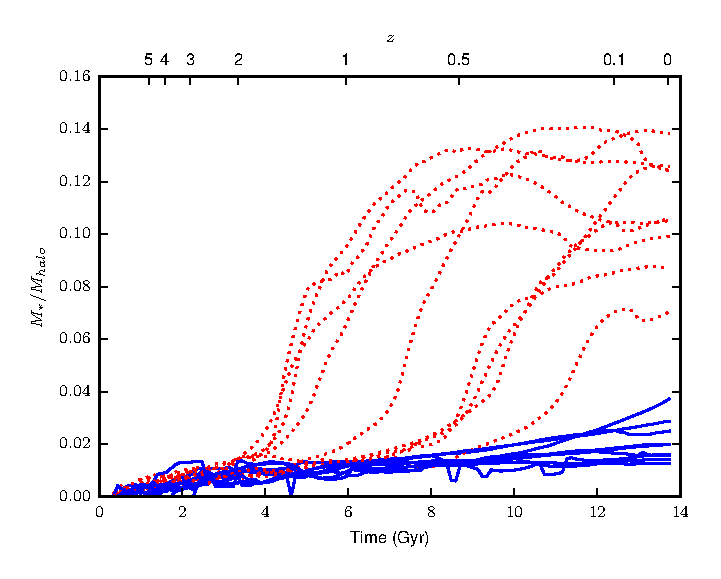
\includegraphics[width=0.8\textwidth]{figures3/stellar_fraction_time.eps}
    \caption[Stellar mass fraction evolution in MUGS2]{Stellar mass fraction
    versus time.  As is clear, for the unregulated population the buildup of
    stellar mass above $\sim3\%$ of the halo mass happens very rapidly, often on
    time-scales of $\sim1\Gyr$.  The runaway in the unregulated population stops
    simply when the disc has been sufficiently depleted of gas that little
    remains to form new stars.}
    \label{stellar_fraction_time3}
\end{figure}
As can be seen in Fig.~\ref{SMHMR3}, roughly half of these galaxies fall within
the expected $z=0$ stellar mass to halo mass relation (SMHMR).  The grey band
shown in the figure is the $2\sigma$ confidence region in the observed SMHMR
from \citet{Hudson2015}, which used the CFHTLens weak lensing survey to produce
a fully-observational SMHMR, without the uncertainties from using the dark
matter-only simulations that are needed for abundance matching techniques (the
\citet{Hudson2015} SMHMR is consistent with past abundance matching estimates
such as \citet{Behroozi2013} and \citet{Moster2013}).  For the rest of this
paper, we will refer to the galaxies that fall within the $2\sigma$ confidence
interval for the observed SMHMR (i.e. galaxies where stellar feedback prevents
overproduction of stars) as {\it well-regulated}, and the galaxies where stellar
feedback fails to produce the correct SMHMR as {\it unregulated}.  No other
criterion is used for determining which population a galaxy falls into. In
addition to overproducing stars, these unregulated galaxies are qualitatively
redder and more bulge dominated, as can be seen in the mock stellar images of
Fig.~\ref{stellar_image3}.  There appears to be no significant difference in
the redshift of the last major merger between the two populations, strongly
suggesting that the failure of stellar feedback to regulate the galaxies is not
simply a matter of recent or violent merging.  The rotation curves in
Fig.~\ref{rotation_curve3} also show the distinct signature of massive bulges
formed by catastrophic angular momentum loss in the unregulated population.
\citet{vanDenBosch2001} showed that this can arise when gas simply traces the
dark matter distribution, without redistribution or ejection by feedback.  The
strong peaks (as high as $700\kms$ for g4720) come about from the central
concentration of baryons in the galaxy bulge.  Without exception, each of the
well-regulated galaxies shows a flat rotation curve, with no evidence of a
significant bulge component.  This matches the qualitative morphology seen in
Fig.~\ref{stellar_image3}.

Fig.~\ref{stellar_central3} shows that for the well-regulated population, the
stellar mass and central baryonic mass follow an extremely tight linear
relation, with a mean star formation efficiency (simply defined here as the
fraction of central baryons that are in stars) of $38\pm2\%$ over a Hubble time.
For the galaxies that fail to self-regulate, they exhibit a total star formation
efficiency of $70\pm10\%$, converting the majority of the baryons that collapse
onto their disc into stars.  Interestingly, the two populations can be divided
cleanly along the $M_{\rm central}=10^{11}\;\Msun$ or the
$M_*=5\times10^{10}\;\Msun$ axis.  This is clear evidence that what explains
the dichotomy here must involve the accretion (or the failure to remove!)
baryons from the central region of the halo, where the disc resides and stars
are formed.  These relations also help to explain some of the correlations seen
observationally, such as the critical mass of $3\times10^{10}\Msun$ that 
\citet{Kauffmann2003a} found dividing star forming and quenched galaxies in the
SDSS at low redshift.

The gas phase diagram of galaxies in the two populations is remarkably similar,
as can be seen in Fig.~\ref{phase3}.  For a representative pair from each
population, of nearly equal halo mass, gas follows essentially the same
evolutionary path, characteristic of a superbubble-regulated ISM, as was shown in
\citet{Keller2015}.  Gas accretes from the halo,
building up a warm ISM at $T\sim10^4\K$.  Where that gas reaches densities of
$\sim 1\;$cm$^{-3}$, it begins to cool quickly and form stars.  Those stars begin to
explode as SN, and a hot superbubble is formed, with $T>10^7\K$.  As the bubble
grows, its temperature falls as it both expands adiabatically and evaporates
the cold shell surrounding it.  This hot, buoyant gas leaves the disc, rising
through the CGM and cooling adiabatically as it goes.  What is remarkable here
is just how similar the phase diagrams of these two galaxies are.  The slight
differences are what we would expect from Table~\ref{z0_table3}.  g19195 has
$\sim50\%$ less gas than g24334, and more than 3 times the SFR at $z=0$.  Thus,
there is less total material, especially in the warm and cold phases, and
slightly more of the very hot ($T>5\times10^7\K$) gas (the interiors of very young
superbubbles) as a consequence of the higher SFR.  What is important to take
away from these phase diagrams is that a well-regulated and unregulated galaxy
do not have any real difference in the phase behaviour of their gas.  There is
no runaway cooling, or failure of SN to generate hot gas:  what causes the
unregulated population to runaway is purely an effect of the outflow
effectiveness, which is set by the depth of the potential well.

\subsection{Time Evolution} 
\begin{figure}
    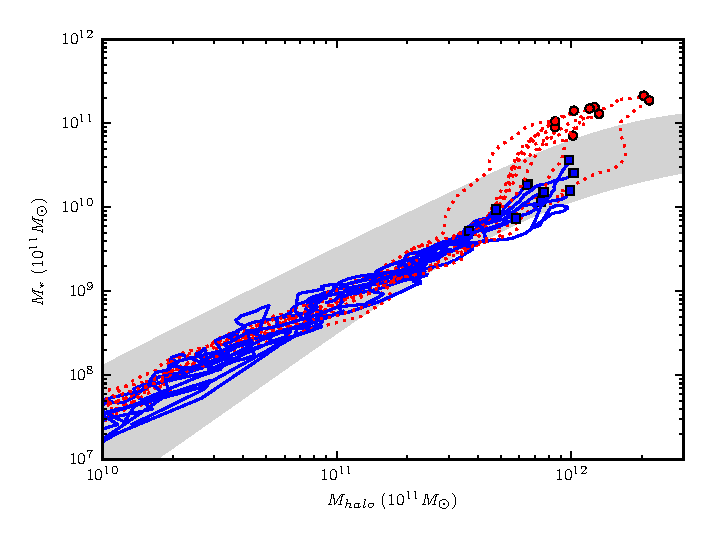
\includegraphics[width=0.7\textwidth]{figures3/SMHMR_time.eps}
    \caption[Stellar mass vs. halo mass evolution in MUGS2]{Stellar mass versus
    halo mass, as shown in Fig.~\ref{SMHMR3}, but with trails added to show time
    evolution.  For halo masses below $\sim\rm{a\;few}\times10^{11}$, the
    evolution of the regulated and unregulated populations are
    indistinguishable.  The grey bar shows the $z=0$ SMHMR, as in
    Fig.~\ref{SMHMR3}}
    \label{SMHMR_time3}
\end{figure}
\begin{figure}
    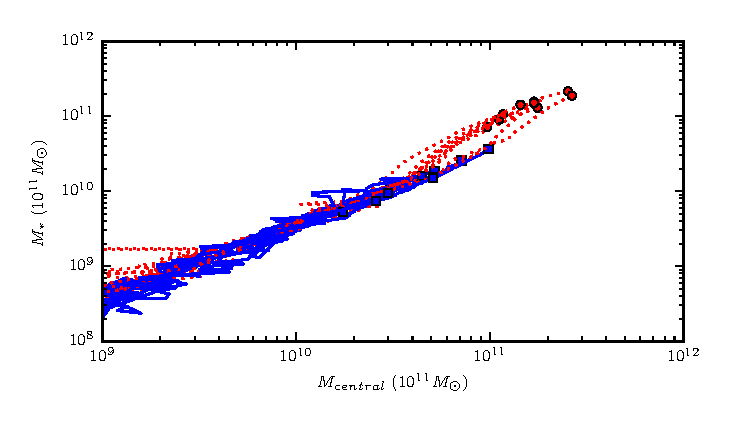
\includegraphics[width=0.8\textwidth]{figures3/stellar_central_time.eps}
    \caption[Stellar mass vs. central baryonic mass evolution in MUGS2]{Stellar
    mass versus central baryon mass. The stellar mass here can be seen to vary
    much more smoothly over the evolution, without the slight `jump' seen in
    Fig.~\ref{stellar_fraction_time3}.  This indicates that both stellar mass
    and central baryonic masses are rapidly increasing together.}
    \label{stellar_central_time3}
\end{figure}

The obvious question that arises from the presence of these two (well-regulated
versus  unregulated) populations at $z=0$ is whether they are distinct through
their entire evolution, and if not, why/how do they diverge?  Previous work
suggests that a characteristic (halo or stellar) mass exists above which AGN
feedback is needed.  There is much uncertainty, however, about where this mass
exactly is, and how the transition from SN to AGN regulation actually works. We
should thus expect galaxies to begin diverging once this characteristic mass is
exceeded.  As Fig.~\ref{stellar_fraction_time3} shows, the stellar mass
fraction for the two populations appear to follow similar evolutionary tracks
for some time (until past $z=0.5$ in the case of g19195, the galaxy which
diverges the latest).  However, once a galaxy begins to overproduce stars, it
appears to do so in a runaway, doubling or even tripling its stellar mass
fraction in less than a Gyr.

The similar early star formation history of the two populations is even more
clear if we look at the SMHMR's time evolution in Fig.~\ref{SMHMR_time3}.  Here
we can see, that for galaxies with halo masses below a few $10^{11}\;\Msun$,
the stellar mass falls well within the expected SMHMR distribution, and the two
populations are indistinguishable.  The mass at which the populations begin to
diverge ( $M_*\sim10^{10}\;\Msun$ and $M_{\rm vir}\sim\operatorname{3-
5}\times10^{11}\;\Msun$) are quite close to the expected transition range
from \citet{Shankar2006} ( $M_*\sim1.2\times10^{10}\;\Msun$ and
$M_{\rm vir}\sim3\times10^{11}\;\Msun$).

The relatively smooth change in the $M_*-M_{\rm central}$ relation, shown in
Fig.~\ref{stellar_central_time3}, shows that it is in fact the central baryon
mass that is more tightly correlated with the stellar mass than the total halo
mass (in galaxies regulated by SN feedback alone). In fact, it is likely that
some of the more massive galaxies in the well-regulated sample are on their way
to failing, but simply have not yet had enough time by $z=0$ to diverge
significantly from the observed SMHMR.  Once more than $\sim10^{11}\Msun$ of
baryons have accreted to the disc of a galaxy, SN alone appear to be unable to
halt the growth of stellar mass.  At this point, star formation efficiency of
the central disc begins to increase, from $\sim40$ to $\sim70$ per cent, resulting in
the differences seen in the two populations at $z=0$.  This accretion crisis, as
it continues to smaller scales, also explains the rotation profiles of the
unregulated population.  The overcollapse that results in runaway star formation
also builds a massive bulge, producing the peaked rotation curves seen in
Fig.~\ref{rotation_curve3}.

\subsection{Galactic Outflows}
\begin{figure}
    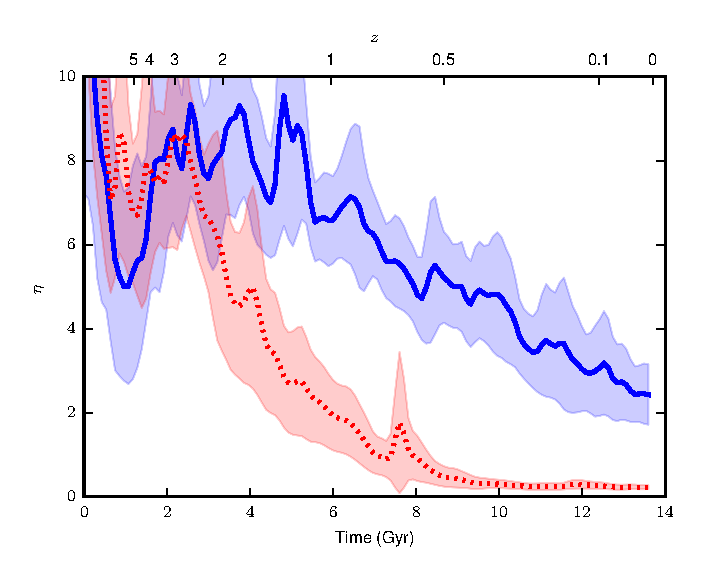
\includegraphics[width=0.8\textwidth]{figures3/massloading_time.eps}
    \caption[Outflow mass loading evolution in MUGS2]{Outflow mass loading
    decreases as galaxies grow over time, as was previously shown by
    \citet{Keller2015}.  Here we see, when examining the mean mass loadings for
    the two populations (the well-regulated galaxies, where stellar feedback
    succeeds, and the unregulated galaxies, where it fails), that the
    unregulated galaxies have their mass loadings decrease sooner, and to lower
    values, than the well-regulated population.  The error bars here are the
    $1\sigma$ scatter in each population.}
    \label{massloading_time3}
\end{figure}
\begin{figure}
    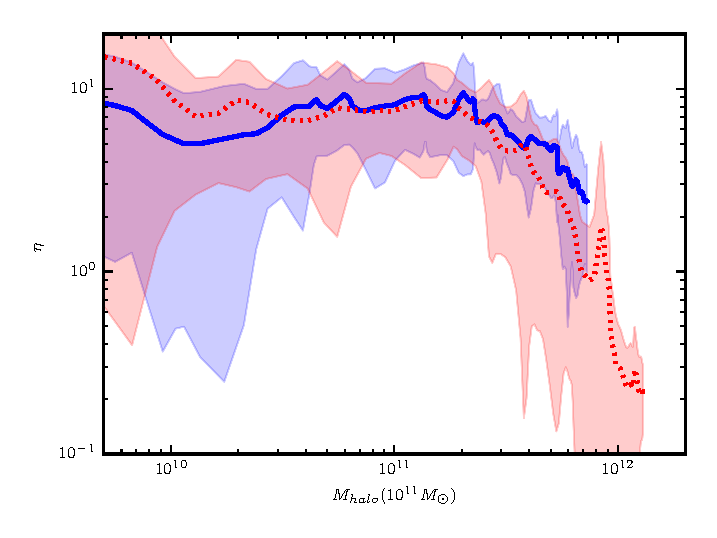
\includegraphics[width=0.8\textwidth]{figures3/massloading_halo.eps}
    \caption[Mass loading as a function of halo mass in MUGS2]{Unlike in the
    previous figure, if we look at mass loading as a function of halo mass, we
    instead see no significant difference between the two populations.  Instead,
    both follow a similar trajectory, and the haloes which fail to self-regulate
    do so simply because they reach a higher mass earlier.}
    \label{massloading_halo3}
\end{figure}

A key metric for both observational and simulation studies of galactic outflows
is the mass loading ($\eta = \dot M_{\rm out} / \dot M_*$) of these outflows.  This
scaling is usually written as a power-law scaling between mass loading $\eta$
and the circular velocity of the halo or halo mass
\citep{Murray2005,Peeples2011}:
\begin{equation}
    \eta \propto v_c^{-\alpha} = (GM_{\rm halo}/R_{\rm vir})^{-\alpha/2} \propto
    M_{\rm halo}^{-\alpha/3}
\end{equation}
The normalization of this relation characterizes how generally effective stellar
feedback is at driving galactic winds and outflows.  The index $\alpha$ is a
measure of how this effectiveness decreases for larger haloes, and ultimately
results in a shutdown of large-scale outflows at high enough mass.  This makes
this scaling relation a key parameter to most semi-analytic galaxy formation
models (e.g \citet{Cole2000}), and an attractive target for both theorists and
observers alike.  Two primary modes for driving galactic winds have been
proposed.  Energy-driven winds (such as those investigated by
\citet{MacLow1988,Tegmark1993}, etc.) assume the cooling times for outflowing
material are shorter than the time required for a superbubble to break out of
the galactic disc.  These adiabatically expanding bubbles result in galactic
winds with mass loadings that scale as $\eta \propto v_c^{-2}$.  A recent study
by \citet{Christensen2016} showed that SN driven winds follow this scaling,
using mock observations of a sample of seven simulated galaxies.  If the cooling
times are instead much shorter than the break out time, then outflows become
momentum driven \citep{Murray2005}, and the mass loadings instead are expected
to scale as $\eta \propto v_c^{-1}$.  \citet{Peeples2011} used a semi-empirical
model to fit the mass--metallicity relationship in low redshift galaxies to
predict that the mass loading index must be $\alpha=3$ or steeper in order to
produce a mass--metallicity relation as steep as is observed.

As in \citet{Keller2015}, we define our outflow rate using the
simple formula below, for gas particles that have $v_r > 0$, and are found
between $0.1R_{\rm vir}$ and $R_{\rm vir}$:
\begin{equation}
    \dot M_{\rm out} = \sum_{r_i\in\mathrm{shell}}\frac{M_i \boldsymbol{v_i}\cdot\hat
    r}{0.9R_{\rm vir}}
    \label{halo_massflux3}
\end{equation}
This choice reflects the nature of these outflows, where gas at high
temperatures and low densities drifts outwards from the galaxy towards
the virial radius.  We chose a relatively thick shell to avoid the need for
frequent simulation outputs.  As such, our ability to resolve short-term bursts
is somewhat reduced, but the overall outflow rates trace those from a test case
with $8\times$ more frequent outputs, and a shell $8\times$ thinner.  An
excellent discussion of how to calculate outflow rates can be found in appendix
A of \citet{Muratov2015}.

If we take the mean mass loadings $\eta = \dot M_{\rm out}/\rm{SFR}$ of our two
populations, we see in Fig.~\ref{massloading_time3} that the mass loading for
the unregulated population drops below $\eta=1$ at $z\sim0.5$, while the
well-regulated population never drops below $\eta\sim2$.  This helps explain the
correlation between the central concentration and stellar mass fraction (in
particular, the dichotomy between the two populations, with low central baryon
masses for well-regulated galaxies and high central masses for the unregulated
galaxies).  Failure to eject gas through outflows gives a higher central baryon
mass, and those baryons inevitably become stars.  However, we know that the
unregulated population is on average heavier (both the full halo, as well as the
central baryons).  Does this earlier drop in outflow mass loading come about
simply because the unregulated population gets heavier earlier?

Fig.~\ref{massloading_halo3} suggests exactly that.  The mass loadings appear
roughly constant, at $\eta\sim10$ for most of the mass-range for both
populations, but begin to fall at essentially the same mass, at what appears to
be the same rate.  An even tighter relation is seen in
Fig.~\ref{massloading_central3}, when the relation between the central baryon
mass, rather than just the halo mass, is examined. It appears that for the
$\eta-M_{\rm halo}$ and $\eta-M_{\rm central}$ relation, a broken power-law fit, as
defined below, describes both the regulated and unregulated population.
\begin{equation}
    \eta = 
    \begin{cases}
        \alpha M^\beta  & \quad \text{if } M < M_0 \\
        (\alpha M_0^{\beta-\gamma}) M^\gamma & \quad \text{if } M > M_0 \\
    \end{cases}
    \label{outflow_scaling3}
\end{equation}
\begin{figure}
    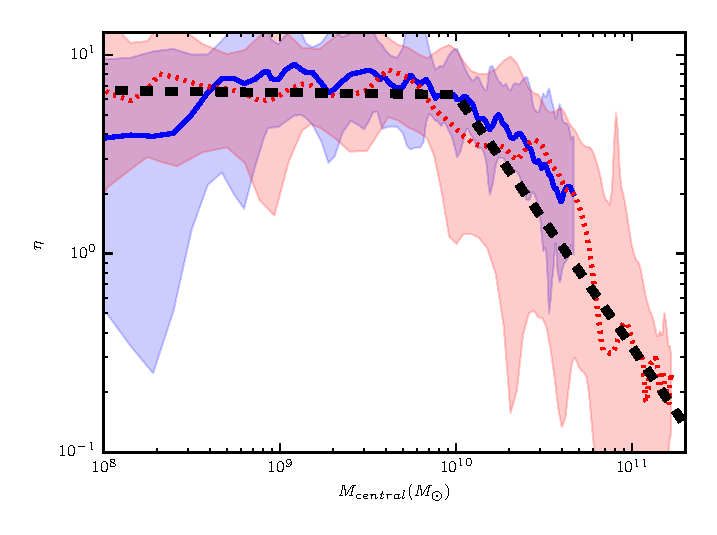
\includegraphics[width=0.8\textwidth]{figures3/massloading_central.eps}
    \caption[Mass loadings as a function of disc mass]{The mass loadings of the two populations are even more in agreement
    if we look at their relation to the central baryonic mass.  As with the mass
    loading versus halo mass relation, we can fit a broken power law to this relation
    (shown here as the dashed line).}
    \label{massloading_central3}
\end{figure}
\begin{figure}
    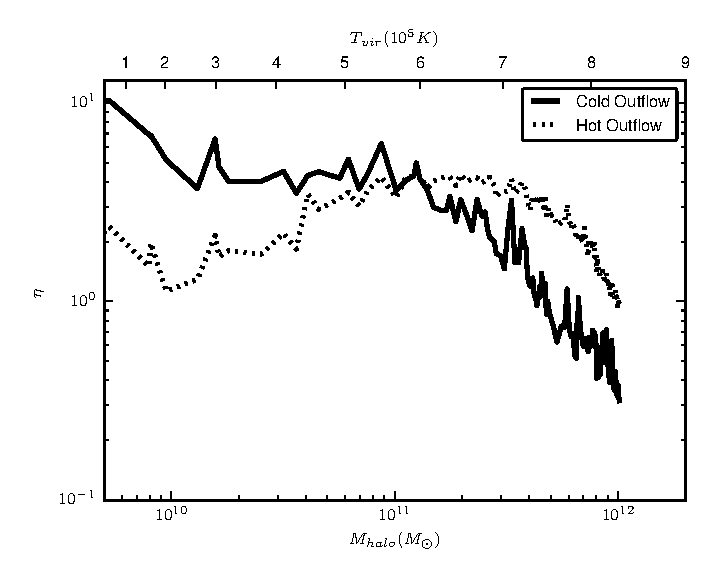
\includegraphics[width=0.8\textwidth]{figures3/coldmassloading.eps}
    \caption[Outflow mass loading for cold and hot gas]{Mean outflow mass loading for the full sample, as a function of
    halo mass/virial temperature, and split into cold ($T<10^5\K$) and hot
    ($T>10^5\K$) components.  For low-mass haloes, outflows are dominated by
    relatively cold gas (cooler superbubbles, and entrained material), while heavier
    haloes have primarily hot outflows.  The transition occurs at a halo mass of
    $M_{\rm halo}\sim10^{11}\;\Msun$, or a virial temperature of $6\times10^5\K$.}
    \label{coldmassloading3}
\end{figure}

Using a simple non-linear least squares fit on the parameters $\alpha$,
$\beta$, $\gamma$, and $M_0$, we find that the most likely value for these
parameters are $\alpha=0.9\pm0.5$, $\beta=-0.01\pm0.06$, $\gamma=-1.3\pm0.1$,
$M_{0}=10^{10.0\pm0.1}$ for the $\eta-M_{\rm central}$ relation, and $\alpha=1\pm1$,
$\beta=0.0\pm0.1$, $\gamma=-1.8\pm0.2$, $M_{0}=10^{11.37\pm0.08}$ for the
$\eta-M_{\rm halo}$ relation.  A fit for both of the populations independently is
consistent with these values derived for the full set of MUGS2 galaxies.
Interestingly, {\it neither} of these slopes is consistent with simple energy
or momentum driven winds (although a single power-law fit does give a slope of
$\sim0.5\pm0.2$, consistent with an energy-driven scenario, albeit with a much
weaker fit).  These values are consistent, however, with the constraints derived
for the mass--metallicity relation and gas content in nearby galaxies derived by
\citet{Peeples2011} (namely, that $\alpha$ in the $\eta\propto v_c^{-\alpha}$
relation be steeper than 3).

The temperature of the outflows also shows an interesting trend as a function of
halo mass.  Fig.~\ref{coldmassloading3} shows that as halo mass increases, the
mass loading of outflows with cold gas monotonically decreases, while the
loading of hot gas is convex, peaking at $M_{\rm halo} =
\operatorname{2-5}\times10^{11}\;\Msun$, and then rapidly falling as halo mass
increases.  We define cold gas as having $T<10^5\K$.  We choose this as a cutoff
point as it lies near the peak of the cooling curve, where we would expect, as
\citet{Woods2014} showed, very little gas to be found.  If we think in terms of
virial temperature, this makes sense.  At low $T_{\rm vir}$, gas around $10^5\K$ is
buoyant, and will be driven out of the disc.  The halo itself is smaller, with a
shallower potential well, thus making it easier for the same amount of feedback
energy to eject a larger amount of entrained gas.  As the halo mass grows,
eventually only the hottest gas is able to escape, and only if it is not weighed
down by too much entrained material.  Eventually, this effect means that the
total mass loading begins to drop significantly.
\begin{figure}
    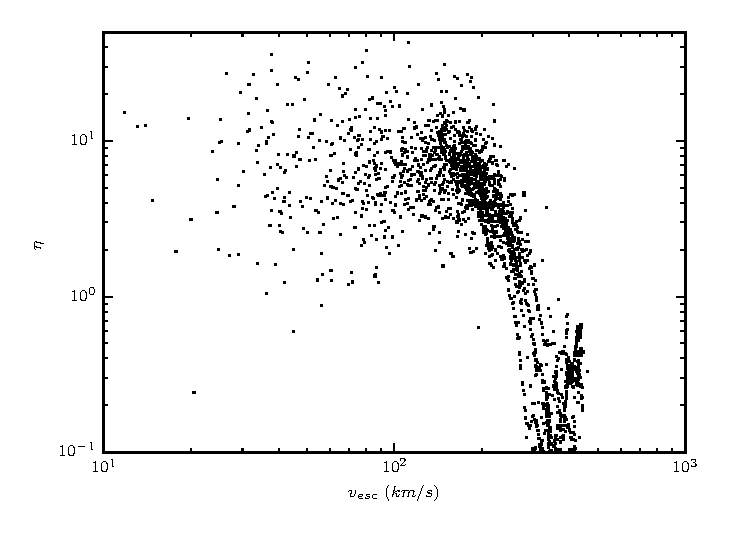
\includegraphics[width=0.8\textwidth]{figures3/massloading_escape.eps}
    \caption[Mass loading vs. escape velocity of disc]{Mean outflow mass loading for the full sample, as a function of the
        escape velocity on the inner surface of our outflow shell
        ($0.1R_{\rm vir}$).  Each galaxy is sampled 128 times over its evolution,
        giving us 2304 points across a range of redshifts.  As can be seen, at
        $v_{\rm esc}\sim 250\;km/s$, the mass loading begins to fall precipitously.
        This corresponds to the sound speed of solar-metallicity gas at a
        temperature of $3.5\times10^{6}\K$.  This means that for gas at or
        above this temperature, sound waves alone are able to propel material
        significantly above the disc, and that kinetic energy losses due to
        shocks will be minimal.  Gas cooler than that will need to be propelled
        supersonically, and will drive shocks in the CGM.}
    \label{massloading_escape3}
\end{figure}

We can see clearly in Fig.~\ref{massloading_escape3} that our winds essentially
have a maximum effective velocity of $\sim250\kms$.  When the escape velocity
at the edge of the galaxy (where we begin to measure outflows, at $0.1R_{\rm vir}$)
exceeds this velocity, outflow mass loadings precipitously drop from $\sim10$ to
$<1$.  As \citet{Keller2014} showed, superbubble-heated gas tends to reach an
equilibrium temperature of a a few million K, meaning that the
outflow rates appear to fall significantly when outflowing gas, moving faster
than the escape velocity from the disc is moving supersonically relative to the
superbubble-heated gas.  Radiative losses from cooling shocks may be important
here for causing the drop in outflow efficiency that produces our two
populations.


\section{Discussion}
In \citet{Keller2015}, we showed that galactic outflows, driven by
pure SN feedback modelled using the superbubble method of \citet{Keller2014} can
produce a moderate mass  $L*$ galaxy with a realistic star formation history and
no significant bulge component.  We have extended this work to a sample
of 18 galaxies, covering a mass range of roughly an order of magnitude around
that first galaxy.  This allows us to probe the expected transition
region, where SN feedback begins to fail as a self-regulation mechanism.

The transition between SN regulated galaxies at low mass and AGN regulated galaxies
at high mass has been studied observationally in the past decade.  \citet{Shankar2006}
found that the relation between halo mass and stellar mass,
$\operatorname{r^*-\rm{band}}$
luminosity, or black hole mass all were characterized by double power laws, with
breaks at $M_{\rm vir}\sim3\times10^{11}\;\Msun$ or $M_*\sim1\times10^{10}\;\Msun$.
They interpreted these results as the transition between the scalings in SN and
AGN regulated galaxies, and constructed a simple analytic model to show the
plausibility of this idea.  \citet{Croton2006} showed that the most massive
galaxies could be produced in a semi-analytic model only when feedback
luminosity no longer simply followed the SFR (as it would in
stellar feedback), but instead scaled with an estimated black hole accretion
luminosity (as one would expect from AGN feedback).  

The most striking feature of this sample of simulated galaxies is the sharp
divide between the two identified populations: the well-regulated galaxies and
the unregulated galaxies.  The well-regulated galaxies are bulgeless and blue,
with a surfeit of extra-planar {\sc Hi} gas.  The unregulated sample are red and
bulge-dominated, with steep rotation curves, with maximum circular velocities as
high as $700\kms$.  The members of the well-regulated population have stellar
mass fractions below $4\%$, while unregulated galaxies have stellar masses all
above $6\%$, with some approaching the cosmic baryon fraction.  Clearly, the
unregulated galaxies do not match the observed properties of $L*$ galaxies in
the nearby universe.  SNe feedback in these galaxies has failed to
prevent runaway bulge growth and star formation.  It has failed because it has
failed to efficiently drive winds, which \citet{Keller2015} showed to be
essential for the formation of a realistic $L*$ galaxy.    As we have assumed no
additional losses in our feedback model it is unlikely that any physically
motivated numerical change to how SN feedback is handled can remove this
dichotomy.

Fig.~\ref{SMHMR3} shows that while the unregulated galaxies tend to be more
massive than the well-regulated ones, there is some overlap in the $M_{\rm
halo}=\operatorname{8-12}\times10^{12}\;\Msun$ range, where there are both
unregulated and well-regulated galaxies.  Figs~\ref{stellar_fraction_time3}
and~\ref{SMHMR_time3} show that the process of runaway star formation happens
rapidly, and can begins over a wide range of halo masses.  This is further
evidence that something beyond simply the mass of the halo that hosts a galaxy
is at play in determining whether or not SN fail to regulate the growth of that
galaxy.

A much tighter correlation is seen when looking at the relation between the
central baryon mass (essentially, the mass of baryons in the galaxy disc), and
the stellar mass fraction.  Figs~\ref{stellar_central3}
and~\ref{stellar_central_time3} show that the stellar mass and central mass are
tightly correlated, and that once the central mass reaches $\sim10^{11}\;\Msun$,
SN feedback will begin to fail.  This is not particularly surprising, as stars
form in the disc, and if SFR occurred at a constant global efficiency, we would
expect to see a correlation between the central baryon mass and the stellar
mass.  However, the two populations show quite different mean star formation
efficiencies, with only $\sim38\%$ of the well-regulated disc baryons existing
in stars compared to $\sim70\%$ in the unregulated population.  This suggests
strongly that the correlations seen between stellar surface density and
quenching \citep{Fang2013} can be set up by SN 
feedback before the AGN begins the quenching process.  It should be noted that
this correlation may simply be a consequence of size evolution
in galaxies, combined with simple quenching dependent only on stellar mass
\citep{Peng2010,Lilly2016}.  In this case too, though, that quenching relation
appears to be initially established by where SN feedback begins to fail.

While propelling
gas beyond the halo's virial radius will certainly ensure that material does not
form stars or collapse through the disc to build a bulge, removing material from
the halo is not necessary to preventing runaway star formation/bulge growth.
Material cycling through the CGM, propelled to a few $100\;\kpc$ above the disc,
can take hundreds of Myr to re-accrete back on to the disc.  This means that the
increasing escape velocity of the disc is more important to preventing outflows
from regulating star formation than an increase in the total halo mass.  A more
massive halo, with a relatively light disc can still have high mass loadings in
its SN-driven outflows, and still have those outflows remove star forming
material from the disc for much a galaxy's life.

\subsection{Outflow Scaling Relations and The End of Regulation}
For gas ejected by stellar feedback, the path out of a galaxy disc is fraught.
To actually escape the disc, buoyant gas must push through the gas above it.
High resolution simulations of disc slices have shown that this means SN
occurring higher above or below the disc drive hotter, faster outflows
\citep{vonGlasow2013,Sarkar2015}.  These results have tended to show that when
feedback is deposited randomly, as opposed to at density peaks, stronger
outflows can be driven.  This is problematic for the simple fact that star
formation should be occurring most vigorously in the densest ISM gas, and this
should therefore be the site of most feedback deposition.  Drift of stars from
their natal environment can give some offset between moderately dense gas and where 
supernovae eventually detonate, but it is unlikely that this is a significant effect
for the majority of stars.  \citet{Governato2010,vonGlasow2013,Christensen2016}
showed that when SN feedback is clustered, it produces stronger outflows
compared to the same number of SN spread distributed more smoothly throughout
the disc.  Unfortunately, even these high-resolution, well controlled studies
have found significant variation in how wind mass loadings scale with halo mass.
The relationship between circular velocity and mass loading has been found to
vary both as a function of how feedback energy is injected \citep{vonGlasow2013}
and what scaling relationship was used to determine halo mass from of the slice
(\citet{Creasey2013} found that using different scaling relations between the
halo mass and surface density could give an index $\alpha$ that varies from 2.5
to 4.8).  These fully cosmological simulations have the advantage of removing
this second source of uncertainty.

The failure of SN to regulate the more massive, disc-heavy galaxies is
ultimately a consequence of the relationship between the efficiency of SN
powered outflows and the mass of the halo (or more precisely, the disc).
Figs~\ref{massloading_halo3} and~\ref{massloading_central3} show that the
outflow mass loading is characterized by a broken power law, with roughly
constant mass loadings at low mass, and mass loadings that follow a power law
with negative slope once a critical mass is exceeded.  This model for outflow
mass loadings is similar to one explored by \citet{Font2011}.  They found that,
in a semi-analytic study of the Milky Way satellites, the best fit for the
observed luminosity function was a so-called `saturated feedback' model, where
mass loadings were flat at low masses, and decreased as a constant power law in
haloes with $v_c>65\kms$ (somewhat lower than the critical value we have
found).  Further evidence against a single power law in the $\eta-M$ relation
came from recent work by \citet{Hou2015}.  By combining the analysis of
\citet{Font2011} along with more recent MW satellite data, the mass--metallicity
relation in local galaxies, and estimates of the redshift of reionization, they
found that only a broken power law for the $\eta-M$ relation can fit all of the
observed data.  Not only that, their `saturated' model resembles quite closely
the fit we have found here, with a flat slope at low masses, and $\eta\propto
M_{\rm halo}^{-1.1}$ for high masses.
\citet{Muratov2015} found a nearly flat $\eta-M_{\rm halo}$ relation
using the FIRE feedback model, with $\eta\propto M_{\rm halo}^{-0.35}$.

This relation seems to arise as a result of different $\eta-M$ relations for
cold and hot gas.  The combination of a steadily decreasing mass loading for
cold gas, combined with hot gas mass loadings that peak at
$M_{\rm halo}\sim5\times10^{11}\;\Msun$ ultimately result in the broken power-law
we see for all outflowing material.  In an upcoming study, we will be examining
how this relation ultimately arises through detailed examination of ultra high
resolution simulations of outflow regions.  A detailed study of the
hydrodynamics of wind venting should determine the processes by which cold ISM
is entrained within the hot outflowing gas, and hopefully explain the origin of
the $\eta-M$ relations we have found here.

The results here also show that even in the unregulated population, superbubbles
are still able to break out of the galaxy disc (as is shown by the adiabatic
evolution of feedback-heated gas seen in Fig.~\ref{phase3}).  In order for a
superbubble to cool adiabatically by a factor of $\sim100$, it must be able to
expand by that same factor, and only once it has left the galaxy disc is there
enough room for it to do this.  The failure of SN feedback in the massive,
unregulated population is an issue of a drop in efficiency, rather than a
complete shutoff, of galactic outflows.  The reason the unregulated population
exists is that the galaxies in this population spent roughly half of their
lifetime above the critical mass in the $\eta-M$ relation, where SN cannot
efficiently drive outflows.  This has resulted in these galaxies becoming too
centrally concentrated, and vastly overproducing stars.
Figs~\ref{coldmassloading3} and~\ref{massloading_escape3} show that at higher
masses (either for the halo itself, or simply for the interior regions), only
the hottest material is able to escape from the disc.  

The $\sim250\kms$ break in mass loading seen in
Fig.~\ref{massloading_escape3} corresponds to the sound speed of relatively hot
gas ($3.5\times10^6\K$ for solar metallicity).  Even with no radiative losses
whatsoever, if $10^{51}\;\rm{erg}$ is deposited into $1000\;\Msun$ of gas (the
specific energy that $\eta=10$ would  yield), this gas would have a temperature
of $2.5\times10^6\K$, and a sound speed of only $\sim210\kms$.  This
temperature is set by the self-regulating process of thermal evaporation, and is
comparable to the internal temperatures seen in other studies of isolated
superbubbles that have included the effects of evaporation
\citep{MacLow1988,Silich1996,Keller2014}.  Thus, it is somewhat unsurprising
that the mass-loadings seen here only stay high for escape velocities below
$200\kms$.  With mass-loadings falling to unity at escape velocities of almost
exactly $300\kms$, we can infer that the total losses (radiatively and
otherwise) between the initial SN explosions and the subsequent outflows are
$\sim80\%$.  The roughly constant outflow rates seen at lower masses/escape
velocities imply that a process other than radiative losses is limiting the
outflow mass-loadings.  The hydrodynamic coupling between hot, outflowing gas
and the surrounding medium (the key process that is involved in setting these
mass loadings) will be the subject of a subsequent study.  Naturally, if
additional feedback energy (i.e. non-SN feedback) is available to heat a
significant amount gas above $\sim3\times10^6\K$, or propel it to speeds
above $\sim250\kms$, this limiting mass will be higher. If radiative or other
losses are higher than what was calculated in these simulations, the limiting
mass will of course be lower.

It should be noted that our selection criteria for haloes (specifically, the
exclusion of haloes with massive neighbours within $2.7\Mpc$), combined with the
use of the zoom-in technique, specifically excludes the environmental effects.
It is known that environmental effects can cause correlations in galaxies
separated by $>5\Mpc$ \citep{Weinmann2006}.  The galaxies here are therefore not
probing the effects of quenching by nearby radio-loud AGN \citep{Kauffmann2015},
or the hot haloes of larger overdensities \citep{Kauffmann2013}.   These limits
therefore may not hold in denser environments, such as the outskirts of a
cluster, where external processes may help regulate star formation.

\subsection{Runaway bulge growth points to AGN feedback}

           
The existence of an unregulated population of galaxies raises the
question of what physical mechanism is missing in these simulations.  What is
important to consider is that this missing physics must be more effective in the
high-mass, bulge dominated unregulated population without causing the low
mass/well-regulated population to underproduce stars, or disrupt their discs.

While CRs rays may be important in certain ISM environments, and may drive
the fastest components of galactic winds, there is no known mechanism involved
in CR feedback that suggests they become more effective at higher mass.  In
particular, there is nothing to suggest that the critical mass we see at
$M_{\rm halo}\sim10^{12}\Msun$ is in any way related to the efficiency or
effectiveness of CR feedback.  For the unregulated population, previous results
suggest that CRs alone will not be able to produce outflows any more
effectively than we have seen SN alone drive, as the mass-loadings they can
produce are typically $\ll10$.  Past simulations have also shown that for the
mass range where SN feedback begins to fail to regulate star formation,
radiation pressure either fails to prevent overproduction of stars
\citep{Aumer2013}, or completely disrupts the thin disc \citep{Roskar2014},
producing `puffy', spherical galaxies with large stellar scale heights,
depending on the details of the subgrid model and how that translates into a
coupling between the photon fluid and the ISM.

The fact that SN begin to fail at relatively high masses hints that the
mechanism that begins to take over in regulating the growth of the galaxy is
AGN.  It has long been suspected that the high-mass end of galaxy evolution was
dominated by AGN feedback from the growth of their SMBHs, and this has been
explored heavily in semi-analytic models
\citep{Bower2006,Croton2006,Shankar2006}.  AGN feedback has also become an
essential component of large-volume simulations, such as EAGLE
\citep{Schaye2015} and Illustris \citep{Sijacki2015}.  Higher resolution
hydrodynamic simulations such as \citet{DiMatteo2005,Ciotti2010,Hopkins2016}
have found that AGN can have dramatic effect on the galactic ISM and star
formation.  A survey of SDSS galaxies with found that the detectable AGN
fraction was essentially zero below $M_*\sim10^{10}\;\Msun$, rising to
$\sim50\%$ by $M_*\sim5\times10^{10}\;\Msun$, with essentially all galaxies
with $M_*>5\times10^{11}\;\Msun$ hosting an AGN \citep{Kauffmann2003b}.  This
transition mass lies exactly where our two populations begin to diverge.  No
galaxy in our sample with $M_*<4\times10^{10}\;\Msun$ is unregulated, and all
but two of the unregulated galaxies have stellar masses above $10^{11}\;\Msun$
(the same effect, at the same stellar mass was seen in the group simulations of
\citep{Liang2016}, which used a prescription for momentum-driven, SN powered
winds).  This is particularly interesting when considering the population of
`powerful' AGN in the SDSS peaks at $M_*\sim10^{11}\;\Msun$.  If these
powerful AGN effectively quench star formation within their host galaxies,
clamping the stellar mass at or below $10^{11}\Msun$, this mechanism would put
essentially all of our unregulated population back within the
\citet{Hudson2015} SMHMR.  If these AGN also ejected a significant fraction of
the gas within the inner $<1\kpc$ of the unregulated population, it would also
solve the problem of their unrealistically large bulges and peaked rotation
curves.  These results suggest that AGN not only {\it can} regulate star
formation and bulge growth in massive discs, they {\it must} do so to produce
realistic galaxies in haloes more massive than $10^{12}\Msun$.

The correlation between black hole mass and bulge mass (see \citealt{Kormendy2013}
for a review of this evidence) is strong evidence that the central regions
co-evolve with with the galaxy (pseudo-)bulge (to first order, this of course
must be the case: they are formed from the same material, in roughly the same
place).  The fact that our unregulated population has grown a much too
massive bulge makes AGN feedback an attractive potential resolution.  In order
to build these massive bulges, angular momentum losses in the gas disc must have
been significant, funnelling material down towards the centre of the disc.  This
naturally would be a necessary component to fuelling the growth of an SMBH, and
powering an AGN.  The well-regulated population likely would
under produce stars if AGN feedback was a strong effect in those galaxies.  
Conveniently, the lack of any sort of significant bulge component means that the
SMBH within those galaxies would likely be starved of fuel, preventing any
significant, sustained AGN feedback.  Further evidence for the negligible effect
of AGN feedback for these smaller galaxies comes again from the SDSS, where it
can be seen that galaxies with $M_*<5\times10^{10}\;\Msun$ contain a powerful
AGN in less than $5\%$ of the cases.

\section{Conclusion}
By correctly modelling SN-driven superbubble feedback, we allow
clustered star formation to efficiently drive outflows.  This allows SN
feedback to produce lower mass galaxies with flat rotation curves, realistic
SMHMRs, and small bulges.  SN feedback breaks down as a regulator of stellar
mass and bulge growth in galaxies with halo masses $>10^{12}\Msun$ (or stellar
masses  $> 4 \times 10^{10}\Msun$).  This breakdown produces a distinct pair of
populations.   Galaxies below these
critical masses have stellar masses within the observed SMHMR, flat rotation
curves, and more mass loaded winds over their evolutionary history.
When simulated with SN feedback alone,  galaxies
above this mass have stellar fractions approaching the cosmic baryon fraction,
redder stellar populations, steeply peaked rotation curves with maximum circular
velocities as high as $700\kms$, and relatively inefficient outflows.  As
massive galaxies grow, they move from the well-regulated to unregulated
population quickly, typically producing the bulk of their stars in a burst
lasting $\le1\Gyr$, after which star formation slows simply due to a dearth of
gas to form stars out of.

The cause for this transition is the relation between the mass loading of
superbubble outflows $\eta$ and the halo or disc mass.  A critical value exists
for both of these masses, where mass loadings begin to drop steeply as mass
increases, reducing the ability of SN to regulate the SFR and baryon content of
the galaxy.  Once the escape velocity from the inner $0.1R_{\rm vir}$ exceeds
$\sim250\kms$, mass loadings fall rapidly to $>1$.  A simple broken power-law
fit describes the relation between the outflow mass loading and both the halo
mass and disc mass.  For disc mass below $10^{10}\Msun$ and halo mass below $2
\times 10^{11}\Msun$, outflow mass loadings are approximately constant, with
$\eta\sim8$.  It is ultimately the mixing driven by thermal evaporation that
sets this mass loading, and the transition mass we have observed here.  These
simulations are the first cosmological sample to explicitly include this physics.
        
SN feedback begins to fail at exactly the mass range that strong AGN are
observationally detected.  This coincides with the runaway growth of massive
stellar bulges in the unregulated population.  The associated black hole feeding
and nuclear activity should not only regulate bulge growth but also the total baryonic
distribution and star formation for galaxies at the high mass end.  
Up to this mass, SN-driven superbubbles alone can regulate the
baryonic content and star formation in galaxies.

If high mass loadings ($\eta\sim10$) are a critical component of galaxy
evolution in nature, then it is energetically impossible for SNe alone to
produce realistic galaxies above the halo masses we have found.  Whether that
mass loading is achieved physically, as we have done with thermal evaporation,
or numerically, the fixed injection energy of SN will ultimately yield a maximum
halo mass, above which SN will be unable to drive winds with high mass loadings.

\section*{Acknowledgements}
The analysis was performed using the pynbody package
(\texttt{http://pynbody.github.io/}, \citealt{pynbody}).  We thank Alyson Brooks,
Fabio Governato, Tom Quinn, and John Kormendy for useful conversations regarding
this paper.  We also thank the referee of this paper for many helpful
suggestions. The simulations were performed on the clusters hosted on
\textsc{scinet}, part of ComputeCanada.  We greatly appreciate the contributions
of these computing allocations.  We also thank NSERC for funding supporting this
research.
\bibliographystyle{mnras}
\bibliography{library}

\chapter{La Fin Du MOND? $\Lambda CDM$ is Fully Consistent with SPARC
Acceleration Law}
\thispagestyle{fancy}
%\setcounter{pageFix}{\value{page}}
\begin{abstract}
\thispagestyle{fancy}
    \setcounter{page}{\value{pageFix}}
        \addcontentsline{toc}{section}{Abstract}
    Recent analysis \citep{McGaugh2016} of the SPARC galaxy sample found a
    surprisingly tight relation between the radial acceleration inferred from
    the rotation curves, and the acceleration due to the baryonic components of
    the disc.  It has been suggested that this relation may be evidence for new
    physics, beyond $\Lambda CDM$.  In this letter we show that the 18
    galaxies from the MUGS2 match the SPARC acceleration relation. These
    cosmological simulations of star forming, rotationally supported discs were
    simulated with a {\sc WMAP3} $\Lambda CDM$ cosmology, and match the SPARC
    acceleration relation with less scatter than the observational data.  These
    results show that this acceleration law is a consequence of
    dissipative collapse of baryons, rather than being evidence for exotic
    dark-sector physics or new dynamical laws.
\end{abstract}

\section{Introduction}
For nearly a century, observations of kinematics in galaxies and clusters of
galaxies have found large velocities inconsistent with the luminous matter
within them.  Even when thorough, comprehensive surveys of the baryonic mass
within galaxies and clusters have been performed, most of the matter has been
found to be missing.  \citet{Zwicky1937} presented observations of galaxy
velocity dispersions in the Coma cluster, and proposed that the bulk of that
cluster's mass was some sort of dark matter (DM).  Later, the groundbreaking
observations of \citet{Rubin1970} showed that this dark matter was also
ubiquitous within disc galaxies like our own.  Today, there is a wealth of
evidence for cold dark matter, not just from galaxy kinematics, but from the
formation of large-scale structure \citep{Blumenthal1984}, the cosmic microwave
background power spectrum \citep{Planck2014},  and the primordial abundances of
elements after Big Bang Nucleosynthesis \citep{Walker1991}.  Dark matter is now
part of the standard cosmology, $\Lambda CDM$, in which most of the
matter in our universe is in fact dark.  Despite this, we still do not know the
actual form that dark matter particles take.  Both direct detection experiments
and searches for dark matter annihilation have failed to conclusively observe
these particles \citep{Aprile2012}, and as such, alternative explanations for
the kinematics of galaxies have been proposed.

The Spitzer Photometry \& Accurate Rotation Curves (SPARC) sample, presented in
\citet{Lelli2016} is a new set of observations and derived mass models for a large
number of rotation-dominated galaxies.  By using $3.6\mu m$ observations, the
stellar mass can be estimated with great accuracy.  The stellar mass is
complemented with $21 cm$ observations of {\sc HI} to get a measure of the gas
mass within the disc. The recent paper by \citet{McGaugh2016}
analyzed this sample, and determined a relation between the observed radial
acceleration determined from the rotation curve ($g_{obs}$), and the
acceleration induced by the baryons observed in the disc ($g_{bar}$).
\citet{McGaugh2016} found that for large values of $g_{bar}$, $g_{obs}\sim
g_{bar}$, while for values of $g_{bar} \lesssim 10^{-10} m\;s^{-2}$, the observed
acceleration begins to rapidly outstrip the acceleration one would expect from
the observed baryons.  They find that the relation between $g_{bar}$ and
$g_{obs}$ is well fit by:
\begin{equation} \label{g_fit}
    g_{obs} = \frac{g_{bar}}{1-\exp{(-\sqrt{g_{bar}/g_\dagger})}},
\end{equation}
where $g_\dagger=1.20\pm 0.26\times10^{-10}\;ms^{-2}$.  In addition to the
simple functional form, \citet{McGaugh2016} find a surprisingly low scatter in
this relation, with residuals normally distributed with $\sigma =
0.11\;\mathrm{dex}$.  The authors noted that this is the same functional form as
the Modified Newtonian Dynamics (MOND) \citep{Milgrom1983} acceleration law,
which attempts to explain galaxy rotation curves without DM.

In discussing these results, \citet{McGaugh2016} offer three possible
explanations for the tight relation. 
\begin{enumerate}
    \item The end point of galaxy formation with conventional (baryonic?)
        physics.
    \item New dark sector physics coupling dark matter and baryons
    \item New dynamical laws (such as MOND
        Tensor-Vector-Scalar Gravity (TeVeS)
        \citep{Bekenstein2004}, etc.)
\end{enumerate}

This is not the first set of observations that appear to be in discordance with
$\Lambda CDM$.  N-body simulations of halo formation have found DM halos follow
a universal, ``cuspy'' density profile \citep{Navarro1996}.  Yet observations of
dwarf galaxies in the local universe find flat, ``cored'' central densities (the
``cusp-core problem'', \citealt{Walker2011}).  Meanwhile, DM-only simulations
were finding that the local group should contain thousands of dwarfs, in
contrast to the dozens actually observed (the ``missing satellites problem''
\citealt{Klypin1999}).  Many of these halos are large enough that suppression of
star formation by reionization could not explain their absence from the
observations (the ``too big to fail'' problem \citealt{Boylan-Kolchin2011}).  

A common feature in each of these conflicts is the comparison of observations to
simulations of galaxy formation that rely purely on N-body, DM-only simulations.
We now know that the impact of baryonic physics, chief among them the feedback
from massive stars and black holes, can have a dramatic effect on the star
formation history (e.g. \citealt{Keller2015}) and density profile of galaxies
\citep{Mashchenko2006}.  Multiple studies \citep[etc]{Pontzen2012,Sawala2016}
have found these problems disappear when galaxies are simulated with gas
dynamics, along with reasonable models for star formation, radiative cooling,
and stellar feedback.  This is what constitutes a modern theory of galaxy
formation, the first of the three options offered to explain the SPARC
acceleration relation.  Galaxies are formed through the gravitational collapse
of collisional particles (gas) into a rotationally supported disc.  Conservation
of angular momentum, combined with star formation and feedback within that disc,
leads to the observed scaling relations and galaxy properties we see today.
Whether this can also reproduce the SPARC acceleration relation has been yet to
be demonstrated.

In this letter, we show that the apparent tension between models of galaxy
formation in $\Lambda CDM$ and the SPARC observations also evaporates when the
collisional collapse of baryons is taken into account.  We find that the
$g_{obs}-g_{bar}$ relation for a set of pre-existing cosmological galaxy
simulations, evolved in a conventional $\Lambda CDM$ cosmology, matches the
SPARC acceleration law, with even tighter scatter than the observed sample.

\section{The MUGS2 Sample}
The McMaster Unbiased Galaxy Simulations 2 (MUGS2) sample is an unbiased,
statistically representative set of 18 cosmological zoom-in simulations of $L*$
disc galaxies.  These galaxies were simulated in a {\sc WMAP3} $\Lambda CDM$
cosmology, with parameters $H_0 = 73\kms \Mpc^{-1}$, $\Omega_M=0.24$,
$\Omega_{bar}=0.04$, $\Omega_\Lambda=0.76$, and $\sigma_8=0.76$.  The MUGS2
$z=0$ halo masses range from $3.7\times10^{11}\Msun$ to $2.2\times10^{12}\Msun$,
with disc masses ranging from $1.8\times10^{10}\Msun$ to
$2.7\times10^{11}\Msun$.  For more details on the creation of the MUGS2 initial
conditions, see the original MUGS paper, \citet{Stinson2010}.  For more
information on the simulations themselves, see \citet{Keller2015,Keller2016}.

MUGS2 was simulated using the modern smoothed particle hydrodynamics code {\sc
Gasoline} \citep{Wadsley2004,Keller2014}.  The simulations used metal line
radiative cooling \citep{Shen2010}, as well as a simple Schmidt law for star
formation.  What sets MUGS2 apart from the original MUGS, aside from improved
hydrodynamics, is the use of a physically motivated, first principles model for
treating feedback from supernovae. (SNe).  Originally presented in
\citet{Keller2014}, the superbubble model captures the effects of thermal
conduction and evaporation between a hot, SNe heated bubble and a surrounding
shell of cold, swept-up interstellar medium (ISM).  This model was derived to allow unresolved
superbubbles to radiatively cool at realistic rates, with no free parameters,
while automatically capturing the effects of clustered SNe.

\subsection{Calculating Accelerations from MUGS2}
In order to compare to the SPARC sample, we located the central halos using the
AMIGA halo finder \citet{Knollmann2009}.  We center the halos using the
shrinking sphere method described in \citet{Power2003}.  Next, in order to
measure rotation curves of the galaxies face-on, we calculate the net angular
momentum vector of all gas within $10\kpc$ of the center of the disk, and rotate
our simulations such that this vector is orthogonal to the x-y plane.
Accelerations were measured in 100 circular annuli $300\pc$ thick.
Accelerations were then calculated using a direct N-body summation on all of the
particles in the halo on those particles within the annulus.  Only the in-plane
component of the acceleration was used, to better follow \citet{McGaugh2016}.
For $g_{obs}$ (the observed acceleration), all particles (gas, stars, and DM)
within the simulation were used.  To calculate $g_{bar}$, we simply calculate
the contributions from stars and gas, $g_*$ and $g_{gas}$, so that
$g_{bar}=g_*+g_{gas}$.  For each of $g_*$ and $g_{gas}$, we use a direct
summation only on those particles (stars and gas respectively).  This process of
direct summation to calculate gravity is equivalent to the numerical solution to
Poisson's equation used in \citep{McGaugh2016}.  The mass model in SPARC
\citep{Lelli2016} included stellar masses estimated from $3.6\;\mu\rm{m}$ near
infrared observations, and gas masses estimated using $21\;\rm{cm}$ observations
of {\sc HI}.  These {\sc HI} masses were converted to total gas masses 
using the simple equation $M_{gas}=1.33M_{HI}$.  Rather than using the total gas
mass from our simulations, we match the {\sc HI}-based estimate from SPARC by
calculating accelerations due to gas using $1.33M_{HI}$, rather than $M_{gas}$.
This is especially important near the outskirts of the galaxy, where the
contribution to the baryonic mass from ionized gas in the ISM and circumgalactic
medium is most significant.  The HI fraction is calculated using the radiative
cooling code within {\sc Gasoline}, which relies on tabulated equilibrium
cooling rates from {\sc CLOUDY} \citep{Ferland2013}.

\begin{figure}
    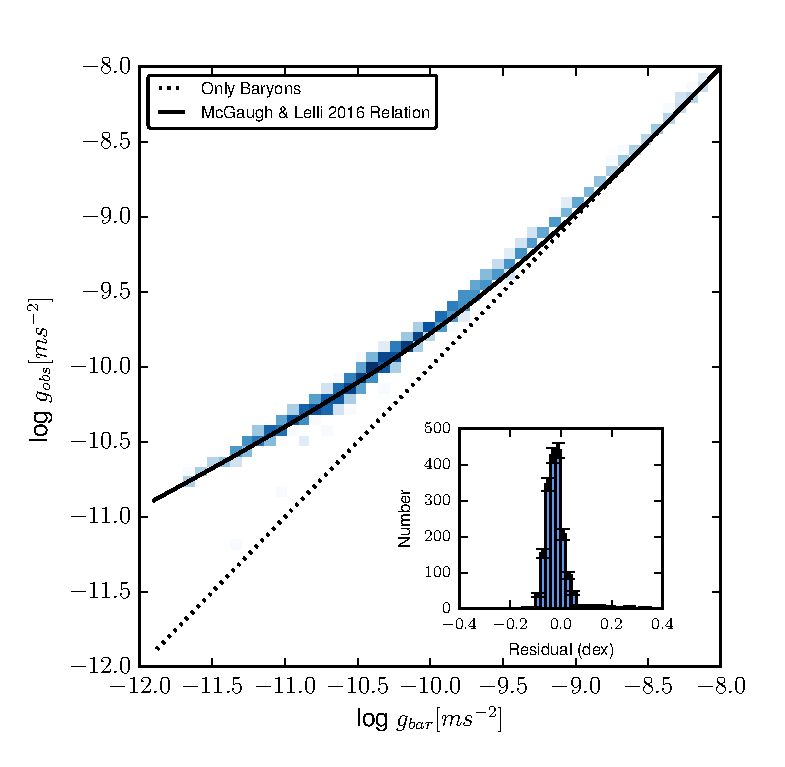
\includegraphics[width=\textwidth]{figures4/SPARC_plot.eps}
    \caption[Total acceleration vs. baryonic acceleration in MUGS2]{Total
    acceleration ($g_{obs}$) vs acceleration due to baryons ($g_{bar}$) from
    1800 data points in the $z=0$ MUGS2 sample, shown in the blue 2-dimensional
    histogram.  The dotted black curve shows the 1:1 relation expected if the
    acceleration was due to baryons alone (without dark matter), while the solid
    line shows the relation presented in \citet{McGaugh2016}.  A Gaussian
    distribution fitted to these residuals finds a variance of $\sigma=0.05$
    dex, significantly lower than the 0.11 dex found by \citet{McGaugh2016}.}
    \label{SPARC_plot}
\end{figure}
\begin{figure}
    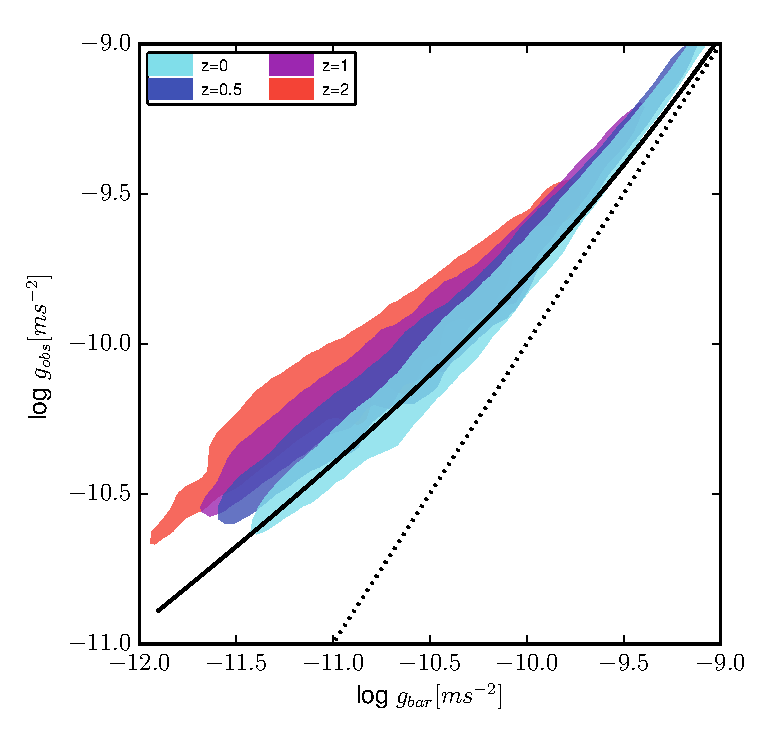
\includegraphics[width=\textwidth]{figures4/redshift_evolution.eps}
    \caption[Redshift evolution of acceleration relation]{The  simulated
    $g_{obs}-g_{bar}$ relation is not constant with redshift.  As this figure
    shows, at higher redshift the low $g_{bar}$ slope is much shallower than at
    $z=0$.  This shows that for high redshift galaxies, their discs can be
    depleted of baryons compared with $z=0$.  We have focused on the low
    $g_{bar}$ end of the relation here, where the changes are most significant.}
    \label{redshift_evolution}
\end{figure}
\begin{figure}
    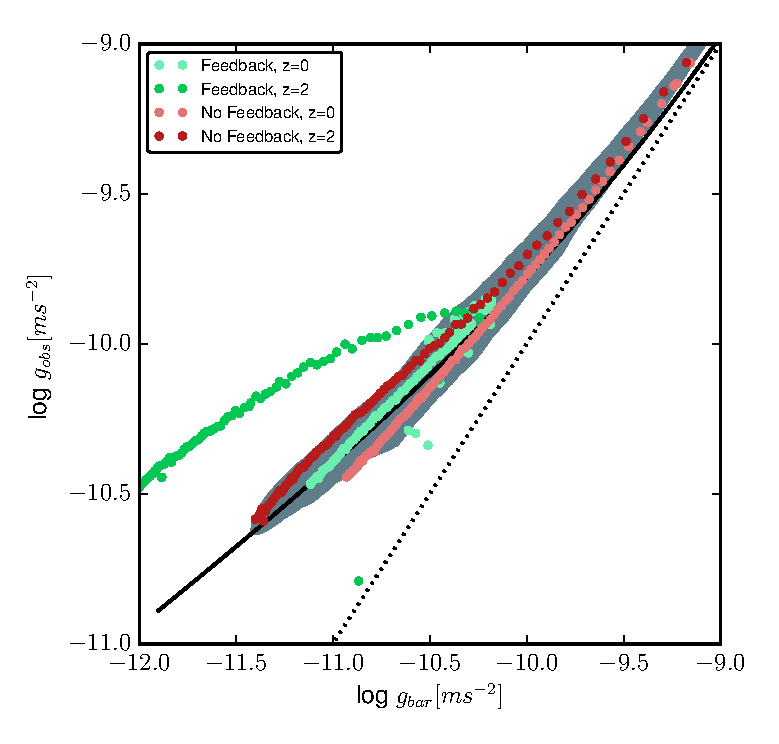
\includegraphics[width=\textwidth]{figures4/FB_effects.eps}
    \caption[Feedback effects on acceleration relation]{The evolution seen in
    figure~\ref{redshift_evolution} is primarily driven by feedback.  This can
    be seen when looking at the same galaxy with and without feedback.  Without
    feedback, the baryon fraction within the disc increases slightly from $z=0$
    to $z=2$, but still roughly follows the SPARC relation.  At $z=2$, strong
    outflows in the galaxy expel most of the baryons from the disc, flattening
    the acceleration relation.  This effect is sensitive to the frequent
    merger-driven starbursts at high redshift, which can drive bursty outflows.}
    \label{FB_effects}
\end{figure}
\section{Results}
\subsection{z=0 Acceleration Relation}
The MUGS2 sample gives us 1800 acceleration data points, just over 2/3 the
sample size of \citet{McGaugh2016}. We show in figure~\ref{SPARC_plot} the
$g_{obs}-g_{bar}$ relation for the MUGS2 sample, compared both to the pure
baryonic acceleration and the SPARC acceleration relation.  It is clear these
simulated galaxies follow the \citet{McGaugh2016} relation {\it extremely} well.
As can be seen from the inset residual distribution, our simulated galaxies
follow the SPARC relation even more tightly than the actual observational data.
The scatter we do see, with $\sigma=0.05$ dex, is consistent with the
\citet{McGaugh2016} estimates.  They decomposed their scatter of $0.11$
dex into different sources, and when all of the observational uncertainties are
removed, the remaining intrinsic scatter gives a variance of $\sigma=0.06$ dex,
very close to the value we find here.  A reduced $\chi^2$ statistic of the SPARC
relation fit to the $z=0$ MUGS2 data finds a very good fit, with $\chi^2_\nu =
1.25$.  These simulation data are fit by equation~\ref{g_fit} at least as well
as the original SPARC data.

\subsection{Feedback \& the Evolution of the Acceleration Relation}
If the SPARC acceleration law is in fact due to new physics, it would be
surprising if the law did not hold at all redshifts.  This would not be the case
if the relation was simply a consequence of galaxy evolution.  In
figure~\ref{redshift_evolution} we show that the acceleration relation in the MUGS2
sample actually shows significant redshift dependence, and only settles to
the equation~\ref{g_fit} relation near z=0.  For these data points, we scaled
the thickness of the annuli by the cosmic scale factor $a$, so that $\delta r =
300a\pc$.  We use this scaling to ensure we are sampling primarily from the
stellar disc, and not well beyond it.  Omitting this scaling has little effect
on these results, save for extending the points to very low values of $g_{bar}$
and removing points from the high $g_{bar}$ end.  This evolution is a
consequence of the huge impact that stellar feedback has on galaxies at
$z\sim2$.  \citet{Keller2015} showed that SNe drive hot outflows from high
redshift galaxies with mass loadings of $\dot M_{out}/\dot M_* \sim 10$.  This
leads to discs at high redshift with baryon fractions depleted relative to those at
low redshift.  This feedback effect is clear when a single galaxy, g1536, is
compared to the same galaxy simulated without SNe feedback.  As
figure~\ref{FB_effects} shows, the redshift trend is nearly nonexistent without SNe
feedback.  Even at $z=2$, the galaxy without feedback falls within the scatter
of the SPARC acceleration law, and within the scatter of the $z=0$ MUGS2
relation.  This tells us that we need not invoke feedback processes to explain
the SPARC acceleration law.  Simple dissipational collapse of gas is sufficient
to produce a similar relation.  The evolution we see as a function of redshift
is therefore dominated primarily by the stronger effect of feedback at higher
redshift.

\section{Discussion \& Conclusion}
We have shown here that the SPARC acceleration law can be produced by conventional
galaxy formation in a $\Lambda CDM$ universe.  Neither the particular functional
form (equation~\ref{g_fit}) nor the small scatter about this relation requires
anything beyond the dissipational collapse of baryons in a DM halo.  The fit
observed at $z=0$ does not hold at all redshifts: vigorous feedback at high
redshift acts to scour protogalaxies of their baryons, reducing the baryon
fraction of the disc, flattening the $g_{obs}-g_{bar}$ relation.  Stellar
feedback is an essential process if we are to produce realistic galaxies.  In order for
a single SPARC law to hold at all redshifts, feedback efficiencies would have to
be so low as to produce galaxies with stellar masses and bulge fractions in
conflict with the observed stellar mass to halo mass relation, and the observed
kinematics of local galaxies. If one wished to use equation~\ref{g_fit} to fit
galaxies at all epochs, $g_\dagger$ would need to have a significant redshift
dependence.  If, on the other hand, high redshift observations of the
$g_{obs}-g_{bar}$ relation found no evolution in shape, or a steeper slope at
low $g_{bar}$, this would in fact constitute a serious disagreement with
$\Lambda CDM$, as it would be difficult to produce the observed low cosmic star
formation efficiency without strong outflows removing baryons from high redshift
discs.

As figure~\ref{FB_effects} shows, the SPARC relation is {\it not} a result of
stellar feedback.  While feedback does change the relationship at high redshift,
its general form is reproduced by simple gas collapse and radiative cooling.
This is one of the few apparent problems in $\Lambda CDM$ that {\it doesn't}
require feedback for its resolution!

\section*{Acknowledgements}
We thank Hugh Couchman and Laura Parker for valuable discussion and suggestions.
The simulations used here were performed on the clusters hosted on
\textsc{scinet}, part of ComputeCanada.  We greatly appreciate the contributions
of these computing allocations.  We also thank NSERC for funding supporting this
research.  

\bibliographystyle{mnras}
\bibliography{library}

\chapter{Conclusion \& Future Work}
\thispagestyle{fancy}
In this thesis, we have explored how supernovae, when modeled with a robust,
physically-motivated method, can impact the growth and evolution of galaxies.
We introduced a novel model for SN feedback that takes into account the
important effects of previously ignored physics: the evaporation of cold gas
driven by thermal conduction.  This model allowed us to see how SN can (and
cannot!) regulate the flow of gas into and out of galaxies, and ultimately
forming stars.  We have also showed that the current $\Lambda CDM$ cosmological
model is consistent with recent observational data.

In Chapter 2, we presented a detailed description of the new superbubble model,
and implemented it in the SPH code {\sc Gasoline2}.  By relying on the strongly
self-limiting process of thermal evaporation \citep{Cowie1977}, where cold mass is evaporated into
a hot bubble with a mass flux given by $ \frac{{\rm d }M_b}{{\rm d}t} =
\frac{4\,\pi\mu}{25k_B}\kappa_0\,\frac{\Delta T^{5/2}}{\Delta x}\ A$, we are
able to develop a new model for SN feedback, that allows realistic estimates for
cooling in unresolved hot bubbles, and accurately calculates the mass loading of
SN energy.  We demonstrated that this model is insensitive to resolution,
unresolved ISM structure, and uncertain turbulent magnetic fields.  Finally,
after investigating the behaviour of individual bubbles, we showed that
superbubble feedback was both more effective at regulating star formation and at
driving galactic winds.

Chapter 3 then applied this new model to the cosmological simulation of a Milky
Way like galaxy.  We compared the same galaxy, simulated four times with
different feedback models (no feedback, the \citet{Stinson2006} blastwave model,
and superbubble feedback with $10^{51}\;\rm{erg}$ and
$2\times10^{51}\;\rm{erg}$).  The results of this comparison found that even
though the galaxy massively overproduced stars (a result previously seen in
\citealt{Stinson2010}) when simulated with blastwave feedback (or no feedback),
the same energy, when simulated using our new superbubble model, was able to
produce a realistic stellar mass fraction for the entire galaxy's history.  Not
only did the galaxy simulated using superbubble feedback have the correct
stellar mass, we showed that it also was effectively bulgeless, with a
completely flat rotation curve.  These two effects were ultimately caused by the
same process.  At high redshift, superbubble feedback efficiently drove highly
mass loaded winds, expelling gas from the ISM of the galaxy.  As the gas that
forms a stellar bulge was primarily accreted at high redshift, this meant that
these winds preferentially removed low angular momentum material, while
preserving the gas with high angular momentum.  This meant that superbubble
feedback was able to naturally prevent both runaway star formation and the
formation of a bulge through these winds.

Chapter 4 took these results to the limit to examine whether SN alone are able
to regulate the formation of stars in galaxies both heavier and lighter than the
Milky Way.  By simulating and examining a new sample of 18 galaxies (the
McMaster Unbiased Galaxy Simulations 2), we were able to demonstrate a critical
mass at which SN feedback breaks down as a regulator of gas accretion and star
formation.  Galaxies that exceed this mass, $\sim 10^{12}\;\Msun$, will produce
more stars than real galaxies, and produce much of these stars in a dense
stellar bulge.  All of this arises due to a fundamental relation between the
mass loading of superbubble driven winds and the mass of the galaxy (either its
halo or its disc).  When the escape velocity of the disc exceeds the sound speed
of superbubble-heated gas (which has a typical mass loading of $\eta=10$), only
outflows which have entrained less material are able to escape the galaxy,
leading to decreasing efficiency in ejecting material, and a shutdown of
SN regulation.  The fact that this shutdown occurs exactly where powerful AGN
are observed, and that it results in a vigorous transport of gas to the nucleus
of the galaxy make this result strong evidence that this shutdown acts as a kind
of ``hand-off'' between SN and AGN feedback.

Chapter 5 applied the new MUGS2 sample of galaxies we produced in
\citet{Keller2016a} and used them to examine the radial acceleration relation
that was derived by \citet{McGaugh2016} from observations of the SPARC
\citep{Lelli2016} catalog.  Contrary to the assertions of some, the tight
relation seen in the SPARC data does not require new fundamental physics (such
as self-interacting dark matter, modified gravity, or MOND).  Instead, the
simply combination of dissipational collapse, together with angular momentum
conservation, means that even galaxies where SN fails to regulate their star
formation (or even where SN are omitted altogether) fall on the observed
relation.  This was the first published demonstration of this in simulation,
using untuned simulations made prior to the publication of \citet{McGaugh2016}.

This thesis has shown that, with correct modelling, SN feedback can regulate the
growth of galaxies up to the mass of the Milky Way, but no further.  In galaxies
up to the mass of our own, SN efficiently drive galactic winds, primarily at
high redshift, that act to limit the availability of low angular momentum gas,
slowing the formation of stars and the stellar bulge. Without the
feedback from SMBHs, galaxies more massive than ours form far too many stars,
and primarily form those stars in a concentrated central bulge.  This transition
from SN to AGN feedback occurs due to a rapid drop in the effectiveness of
SN-driven outflows.  Finally, we showed that independent of the detailed
internal processes of galaxy evolution, the acceleration relation observed by
\citet{McGaugh2016} is simply a natural consequence of galaxy formation.

\section{Future Directions}
These results will be useful for many new research projects.  The superbubble
model is a robust tool for simulating galaxies, and will become a key part of
future studies using the simulation codes {\sc Gasoline2} and {\sc ChaNGa}.  The
MUGS2 sample is a useful new set of simulations for answering questions
involving the evolution of Milky Way-like galaxies (as evidenced by our use of
it in Chapter 5).  These two resources will be valuable to both myself and other
researchers for years to come. The four publications presented here point
towards a number of questions I plan to answer during my postdoctoral research.  

While observational evidence abounds for the existence of SMBHs
\citep{Kormendy2013}, and the impact of the AGNs they power
\citep{Veilleux2005}, there is still great uncertainty as to the details of how
they regulate their own growth, and the growth of the galaxies they live in.
\citet{Keller2016a} showed evidence that a transition occurs between galaxies
regulated by SN feedback to AGN feedback as they grow heavier than the Milky
Way.  How this handoff occurs remains widely unexplored.  Using my superbubble
feedback, along with new models for SMBH growth \citep{Hopkins2010} and
migration \citet{Tremmel2015}, we will for the first time be able to simulate
the growth of SMBHs in galaxies with first-principles, physically motivated
physics.  This will allow us to study the full gamut of galaxies that exist, and
study how the tight scaling relations between stellar bulges and SMBHs might
arise.

The CGM gas that surrounds galaxies is the interface between the star forming
disc and the galaxy's hot, gaseous halo (and the cosmic web beyond).  Any
material that accretes from the halo must first pass through the CGM, and any
material that leaves the ISM first does so into the CGM.  Despite the importance
of this component of the galaxy, observations of gas in the CGM are difficult.
This gas tends to be too cool \& diffuse to be a strong emitter of X-rays, and
absorption line studies require the lucky coincidence of a background quasar
\citep{Weiner2009}.  In addition to this, we know that the CGM contains complex,
multiphase structure, including cool neutral clouds \citep{Wakker1997},
molecular gas \citep{Stark1984}, and dust .  How this material can persist in a
CGM that is much hotter, and that may be shearing past at supersonic velocities
is currently an open question.  Analytic calculations \& high resolution
simulations suggest that these clouds should be disrupted and mixed on
timescales far shorter than is required to ballistically launch them into the
CGM.  In light of this, why do we see these clouds?  They may be formed in-situ,
or may be launched by the fragmentation of superbubble shells, already
accelerated to high velocities during the momentum-conserving snowplow phase of
the bubble's growth.  High resolution simulations of superbubble breakout from
the ISM will be able to tell us if this is indeed the origin of these clouds.
Understanding the details of the multiphase CGM is key to
understanding how galaxies accrete and expel gas, as thermal instability in the
CGM (which depends heavily on its density, temperature, and metallicity) may be
the mechanism by which spiral galaxies today aquire the gas required to
form new stars \citep{Marasco2012}.


Large volume simulations like Illustris \citep{Vogelsberger2014b} and EAGLE
\citep{Schaye2015} can show how whole populations of galaxies evolved from the
earliest linear structures.  While these simulations contain models for star
formation, feedback from both stars and AGN, as well as radiative cooling, these
have all been fine-tuned to fit observed scaling relations.  This limits the
ability of these simulations to explain the origins of the observations they
have been tuned to fit.  My superbubble model contains no free/tuned parameters,
and accurately captures the evolution of feedback-heated gas as it evaporates
cool material that surrounds it.  It is the only feedback model currently in
existence that captures the important physical process of thermal conduction and
evaporation.  It will allow us to build a statistically significant sample of
physically realistic galaxies.  With first-principles, physically motivated
models for the unresolved physics in our simulations, we will be able to study
the actual physics involved in shaping both individual galaxies and the
populations that we observe. 
\bibliographystyle{mnras}
\bibliography{library}


\end{document}
